% This must be in the first 5 lines to tell arXiv to use pdfLaTeX, which is strongly recommended.
\pdfoutput=1
% In particular, the hyperref package requires pdfLaTeX in order to break URLs across lines.

\documentclass[twocolumn]{article}

% Change "review" to "final" to generate the final (sometimes called camera-ready) version.
% Change to "preprint" to generate a non-anonymous version with page numbers.
\usepackage[preprint]{acl}

% Standard package includes
\usepackage{times}
\usepackage{pdfpages}
\usepackage{latexsym}
\usepackage{array}
\usepackage{lipsum}  
\usepackage{makecell}
\usepackage{booktabs}
\usepackage{graphicx}
\usepackage{caption}
\usepackage{booktabs}
\usepackage{xcolor}
\usepackage{enumitem}
% \usepackage[margin=1in]{geometry}
\usepackage{array}
\usepackage{longtable}
\usepackage{natbib} 
\usepackage{standalone}
\usepackage{subcaption}
\usepackage{tikz}
\usepackage{pgfplots}
\pgfplotsset{compat=1.18}
\usepackage{array}
\usepackage[ruled,vlined]{algorithm2e}
\usepackage{colortbl}  % For row colors
\usepackage{array}     % For better table formatting
\usepackage{amsmath}
\usepackage{booktabs}  % For better table formatting
% For proper rendering and hyphenation of words containing Latin characters (including in bib files)
\usepackage[T1]{fontenc}
\SetCommentSty{textit}  % Make comments italic
\SetVlineSkip{0.5em}   % Adjust vertical line spacing
% For Vietnamese characters
% \usepackage[T5]{fontenc}
% See https://www.latex-project.org/help/documentation/encguide.pdf for other character sets

% This assumes your files are encoded as UTF8
\usepackage[utf8]{inputenc}

% This is not strictly necessary, and may be commented out,
% but it will improve the layout of the manuscript,
% and will typically save some space.
\usepackage{microtype}

% This is also not strictly necessary, and may be commented out.
% However, it will improve the aesthetics of text in
% the typewriter font.
\usepackage{inconsolata}

%Including images in your LaTeX document requires adding
%additional package(s)
\usepackage{graphicx}
% \usepackage{algorithm}
% \usepackage{algorithmic}
\usepackage{algpseudocode}
\usepackage{multirow}
\usepackage{tabularx}   % For tables with adjustable-width columns
\usepackage{amsmath}
\usepackage[utf8]{inputenc}
\usepackage{verbatim} % or use the listings package if preferred
\usepackage{amsthm}
\usepackage{amssymb}
\usepackage{pifont}
\usepackage{fontawesome}
% \usepackage{bbding}
% \usepackage{tcolorbox}
% \usepackage{xcolor}
% \usepackage{fontawesome}

% Optional: If you want to customize the algorithm appearance
\renewcommand{\algorithmicrequire}{\textbf{Input:}}
\renewcommand{\algorithmicensure}{\textbf{Output:}}
\setlength{\parskip}{0.5em} % Or whatever value you prefer
% If the title and author information does not fit in the area allocated, uncomment the following
%
%\setlength\titlebox{<dim>}
%
% and set <dim> to something 5cm or larger.


\title{MedHallu: A Comprehensive Benchmark for Detecting Medical Hallucinations in Large Language Models}

% Author information can be set in various styles:
% For several authors from the same institution:
% \author{Author 1 \and ... \and Author n \\
%         Address line \\ ... \\ Address line}
% if the names do not fit well on one line use
%         Author 1 \\ {\bf Author 2} \\ ... \\ {\bf Author n} \\
% For authors from different institutions:
% \author{Author 1 \\ Address line \\  ... \\ Address line
%         \And  ... \And
%         Author n \\ Address line \\ ... \\ Address line}
% To start a separate ``row'' of authors use \AND, as in
% \author{Author 1 \\ Address line \\  ... \\ Address line
%         \AND
%         Author 2 \\ Address line \\ ... \\ Address line \And
%         Author 3 \\ Address line \\ ... \\ Address line}

% \author{First Author \\
%   Affiliation / Address line 1 \\
%   Affiliation / Address line 2 \\
%   Affiliation / Address line 3 \\
%   \texttt{email@domain} \\\And
%   Second Author \\
%   Affiliation / Address line 1 \\
%   Affiliation / Address line 2 \\
%   Affiliation / Address line 3 \\
%   \texttt{email@domain} \\}

\author{
 \textbf{Shrey Pandit\textsuperscript{1}\thanks{Corresponding author: \href{mailto:shreypandit@utexas.edu}{shreypandit@utexas.edu}}},
 \textbf{Jiawei Xu\textsuperscript{1}},
 \textbf{Junyuan Hong\textsuperscript{1}},\\
 \textbf{Zhangyang Wang\textsuperscript{1}},
 \textbf{Tianlong Chen\textsuperscript{2}},
 \textbf{Kaidi Xu\textsuperscript{3}},
 \textbf{Ying Ding\textsuperscript{1}}
% \\
%  \textbf{Fifth Author\textsuperscript{1,2}},
%  \textbf{Sixth Author\textsuperscript{1}},
%  \textbf{Seventh Author\textsuperscript{1}},
%  \textbf{Eighth Author \textsuperscript{1,2,3,4}},
%\\
%  \textbf{Ninth Author\textsuperscript{1}},
%  \textbf{Tenth Author\textsuperscript{1}},
%  \textbf{Eleventh E. Author\textsuperscript{1,2,3,4,5}},
%  \textbf{Twelfth Author\textsuperscript{1}},
%\\
%  \textbf{Thirteenth Author\textsuperscript{3}},
%  \textbf{Fourteenth F. Author\textsuperscript{2,4}},
%  \textbf{Fifteenth Author\textsuperscript{1}},
%  \textbf{Sixteenth Author\textsuperscript{1}},
%\\
%  \textbf{Seventeenth S. Author\textsuperscript{4,5}},
%  \textbf{Eighteenth Author\textsuperscript{3,4}},
%  \textbf{Nineteenth N. Author\textsuperscript{2,5}},
%  \textbf{Twentieth Author\textsuperscript{1}}
\\
\faGlobe~Dataset \& Code: \url{https://medhallu.github.io/} \\
 \textsuperscript{1}University of Texas at Austin,
 \textsuperscript{2}UNC Chapel Hill,
 \textsuperscript{3}Drexel University,
 % \textsuperscript{4}Affiliation 4,
 % \textsuperscript{5}Affiliation 5
% \\
 % \small{
 %      Data and Code: \href{https://medhallu.github.io/}{https://medhallu.github.io/}
 % }
}


\begin{document}
\maketitle
\begin{abstract}
Advancements in Large Language Models (LLMs) and their increasing use in medical question-answering necessitate rigorous evaluation of their reliability. A critical challenge lies in hallucination, where models generate plausible yet factually incorrect outputs. In the medical domain, this poses serious risks to patient safety and clinical decision-making. To address this, we introduce \textbf{MedHallu}, the first benchmark specifically designed for medical hallucination detection. MedHallu comprises 10,000 high-quality question-answer pairs derived from PubMedQA, with hallucinated answers systematically generated through a controlled pipeline. Our experiments show that state-of-the-art LLMs, including GPT-4o, Llama-3.1, and the medically fine-tuned UltraMedical, struggle with this binary hallucination detection task, with the best model achieving an F1 score as low as 0.625 for detecting ``hard'' category hallucinations. Using bidirectional entailment clustering, we show that harder-to-detect hallucinations are semantically closer to ground truth. Through experiments, we also show incorporating domain-specific knowledge and introducing a ``not sure'' category as one of the answer categories improves the precision and F1 scores by up to 38\% relative to baselines. 
% The MedHallu benchmark is publicly accessible at [LINK].
\end{abstract}

\section{Introduction}
Recent advances in Large Language Models (LLMs)~\citep{achiam2023gpt} have catalyzed their widespread adoption as assistive tools across a multitude of domains, including software development~\citep{Krishna_2024_software}, healthcare ~\citep{singhal2022largelanguagemodelsencode_health}, weather prediction~\citep{li2024cllmatemultimodalllmweather}, and financial applications \citep{nie2024surveylargelanguagemodels}. However, LLMs are prone to hallucination~\citep{bang2023multitaskmultilingualmultimodalevaluation_hallucination}, where they generate plausible but factually incorrect or unverifiable information~\citep{Ji_2023_12RW, Huang_2025_survey11}. Hallucinations can arise from various factors, including biased or insufficient training data~\citep{han2024skipnsimplemethod_data, zhang2024knowledgeovershadowingcausesamalgamated_data}, and inherent architectural limitations of LLMs \citep{leng2023mitigatingobjecthallucinationslarge_architecture, kalai2024calibratedlanguagemodelshallucinate_architecture}. This issue is particularly problematic in high-stakes fields such as the medical domains, where the generation of incorrect information can exacerbate health disparities~\citep{singhal2022largelanguagemodelsencode_health}. 

 % Efforts to address hallucination involve implementing strategies such as Retrieval-Augmented Generation \citep{Semnani_2023_RAG_Hallu}, self-refinement techniques \citep{huang2022largelanguagemodelsselfimprove} \citep{wang2023selfconsistencyimproveschainthought}, and rigorous fine-tuning on factual datasets. These approaches aim to enhance the reliability of AI outputs in healthcare settings. Nonetheless, challenges remain in ensuring the scalability and generalizability of these strategies, highlighting the need for ongoing research and development in the field.

\begin{figure}[t]
\centering
\includegraphics[width=1\linewidth]{figures/figure_1.pdf}
\caption{An example of medical hallucination detection. The detailed prompt used for the hallucination detection task is presented in Appendix \ref{appendix:prompt}.}
\label{fig:task}
\end{figure}

Detecting hallucinations in LLM outputs (Figure~\ref{fig:task}) is therefore of critical importance. Various methods have been proposed to address this issue, including self-consistency~\citep{wang2023selfconsistencyimproveschainthought}, sampling-based approaches such as SelfCheckGPTZero \citep{manakul2023selfcheckgptzeroresourceblackboxhallucination_detect1}, and intrinsic methods that evaluate token-level uncertainty and entropy~\citep{azaria2023internalstatellmknows_detect2, xiao2021hallucinationpredictiveuncertaintyconditional_detect3}.
Existing benchmarks, such as HaluEval~\citep{Hallueval} and Haydes~\citep{liu2022tokenlevelreferencefreehallucinationdetection} primarily evaluate hallucination detection capabilities on general tasks, including summarization, question answering, and dialogue systems, with an emphasis on common-sense knowledge rather than domain specificity. 
% \kaidi{the following paragraph is very important, please use \ding{202} \ding{203} \ding{204} to oragnize them}  
This gap becomes particularly consequential in the medical domains, where specialized terminology requires precise handling, as minor lexical deviations can lead to substantially divergent interpretations~\citep{singhal2022largelanguagemodelsencode_health}. While recent efforts such as HaluBench~\citep{ravi2024lynxopensourcehallucination}, incorporate limited samples from the medical domains, their domain-agnostic generation frameworks lack medical curation. Similarly, Med-Halt~\citep{pal2023medhaltmedicaldomainhallucination} focuses on model benchmarking rather than providing a structured evaluation resource. Furthermore, the subtlety of hallucinations (e.g., whether they are hard or easy to detect) remains underexplored in the medical context. Additionally, the performance differences between pre-trained LLMs and fine-tuned medical LLMs are sparsely documented~\cite{ravi2024lynxopensourcehallucination, Hallueval, pal2023medhaltmedicaldomainhallucination}.

To address these gaps, we present the \textbf{Med}ical \textbf{Hallu}cination detection dataset (\textbf{MedHallu}), a comprehensive corpus of 10,000 medical question-answer pairs derived from the established PubMedQA dataset. Each pair is meticulously annotated to distinguish accurate responses from hallucinated content. Furthermore, MedHallu is stratified into easy, medium, and hard detection tiers based on the subtlety of hallucinations, enabling granular evaluation of model capabilities. The primary contributions of this research are threefold:
 \begin{itemize}
 \vspace{-3mm}
     \item We introduce MedHallu, one of the first datasets specifically designed for medical hallucination detection tasks. Comprising 10,000 entries derived from PubMedQA, MedHallu is systematically categorized into three levels of difficulty—easy, medium, and hard—based on the subtlety of hallucination detection.

     \item We find that hallucinated answers that are semantically closer to the ground truth are more challenging to detect. Furthermore, clustered answers using bi-directional entailment reveal uniformity, where all entries in a cluster are consistently either easy or hard to detect.

    \item Our evaluation shows that general-purpose LLMs outperform fine-tuned medical LLMs in medical hallucination detection tasks. Additionally, we find that model performance can be enhanced by providing relevant knowledge to LLMs. Moreover, introducing a ``not sure'' class alongside the existing classes of ``hallucinated'' and ``not-hallucinated'' leads to improved precision, which is critical in the medical domains.

 \end{itemize}

% \shreyp{WRITE SOMETHING ABOUT PAST WORK AND RESEARCH GAP}
% We further analyze the similarity between the hallucinated and ground truth samples by clustering the hallucinated answers using the bidirectional entailment method~\citep{Farquhar2024DetectingHI_semantic_entropy}. We find that hallucinated points that are harder to distinguish are semantically closer to the ground truth in metrics such as Euclidean distance, higher cosine similarity score, and high Rouge-2 score than those that are easy to detect, giving insights on LLMs discriminatory behavior, pointing to that it is the semantic meaning of a sentence that is resulting in difficult detection rather than syntactic behavior. 

% Previous works such as HaluBench \citep{ravi2024lynxopensourcehallucination}, HaluEval \cite{Hallueval}, and Med-HALT \citep{pal2023medhaltmedicaldomainhallucination} have primarily focused on examining general-purpose LLMs for their ability to detect hallucinations. These studies have not examined how domain-specific Large Language Models perform in these tasks. To address this gap, we assess fine-tuned medical LLMs, mainly Med42-8B \citep{med42v2}, Meditron3-8B, OpenBioLLM-8B \citep{OpenBioLLMs} and UltraMedical-8B \citep{zhang2024ultramedical} in the context of medical hallucination detection task as described in figure \ref{fig:task}, and discover that their performance is inferior to that of their instruction-tuned counterparts. Our methodology for dataset creation is detailed in Section \ref{Methodology}.


 
\begin{figure*}[ht]
\centering
\includegraphics[width=1\linewidth]{figures/figure_2.pdf}
\caption{\textbf{MedHallu} medical hallucinated answer generation pipeline. Each question-answer pair from the PubMedQA dataset undergoes the following steps to generate a hallucinated answer: (1) \textbf{Candidate Generation}: Given a question, relevant knowledge, and ground truth answer, the LLM is prompted to generate a hallucinated answer adhering to one of four hallucination types. (2) \textbf{Grading \& Filtering}: Generated answers undergo \textbf{quality} and \textbf{correctness} checks, being labeled as \textbf{hard}, \textbf{medium}, \textbf{easy}, or \textbf{failed} based on filtering results. (3) \textbf{Refining Failed Generation}: Failed answers are optimized using TextGrad~\cite{yuksekgonul2024textgradautomaticdifferentiationtext} and re-filtered. If they fail again, the LLM is re-prompted to generate new answers (\textbf{Regeneration}). (4) \textbf{Fallback}: If no qualified answers emerge after four regeneration attempts, the answer most similar to the ground truth is selected as an easy hallucinated example. The detailed prompt used for hallucination generation task is presented in the Appendix~\ref{appendix:prompt}.}
\label{fig:pipeline}
\end{figure*}

 % \begin{table}[h]
    \centering
    \small
    \renewcommand{\arraystretch}{1.2}  % Increases row spacing
    \begin{tabular}{|>{\raggedright\arraybackslash}p{0.1\textwidth}|>{\raggedright\arraybackslash}p{0.3\textwidth}|}
        \hline
        \rowcolor{gray!10} \textbf{Component} & \textbf{Content} \\
        \hline
        \textit{Question} & Is halofantrine ototoxic? \\
        \hline
        \textit{Ground Truth} & Halofantrine has mild to moderate pathological effects on cochlea histology, can be considered ototoxic drug. \\
        \hline
        \textit{Hallucinated Answer} & Halofantrine exhibits no ototoxicity and is generally considered safe for auditory function. \\
        \hline
    \end{tabular}
    \caption{An example in the MedHallu dataset.}
    \label{tab:dataset-example}
\end{table}
\vspace{-3mm}
\section{Related Work}
\vspace{-2mm}
\paragraph{Hallucination Detection Benchmarks.}
 Hallucination in LLMs has been extensively documented in a variety of tasks, including machine translation~\citep{lee2019hallucinations_13RW}, dialogue systems~\citep{balakrishnan-etal-2019-constrained_14RW}, text summarization~\citep{durmus-etal-2020-feqa_15RW}, and question answering~\citep{sellam2020bleurtlearningrobustmetrics_16RW}, as reviewed in recent surveys~\citep{Ji_2023_12RW}. Existing benchmarks for hallucination detection, such as Hades~\citep{liu2022tokenlevelreferencefreehallucinationdetection} and HaluEval~\citep{Hallueval}, offer robust methodologies for identifying hallucinated content. However, they predominantly employ generic techniques that fail to account for the nuanced complexities inherent in medical contexts. Similarly, while benchmarks such as HaluBench~\citep{ravi2024lynxopensourcehallucination} include some medical data samples in their data set, their data generation processes are not specifically tailored for the medical domain. Although Med-HALT~\citep{pal2023medhaltmedicaldomainhallucination} focuses on medical hallucinations, it mainly serves as a performance evaluation tool rather than providing a structured dataset. In contrast, our work introduces the first comprehensive dataset for medical hallucination detection, employing controlled methods to address these domain-specific challenges.
\vspace{-2mm}
\paragraph{Semantic Analysis of Hallucinated Text.}
Hallucinated sentences often sound over-confident~\citep{miao2021preventlanguagemodeloverconfident_overconfident, chen2022improvingfaithfulnessabstractivesummarization_overconfident} and frequently contain tokens that are statistically improbable within a given context, primarily due to suboptimal decoding strategies. Fine-tuned models have sought to mitigate this issue by adjusting decoding parameters to enhance factual accuracy, thereby reducing the occurrence of rare or anomalous terms in hallucinated outputs~\citep{Huang_2025_survey11}. Despite these advancements, previous research has not systematically compared hallucinated sentences with their corresponding ground truth to assess semantic similarities. Our work fills this gap by uncovering deeper semantic relationships between hallucinated texts and their ground truth counterparts.
\vspace{-2mm}

\paragraph{Improvement Methods in Hallucination Detection.}

Recent advancements in hallucination detection have focused on integrating external knowledge to enhance model performance. Retrieval-augmented methods~\citep{lewis2021retrievalaugmentedgenerationknowledgeintensivenlp_241, li2023weboysterimprovinglarge_242} have mitigate hallucinations via grounding models in general knowledge. However, few studies have examined the impact of domain-specific knowledge on hallucination detection tasks. While HaluEval~\citep{Hallueval} evaluates knowledge-augmented detection, it lacks fine-grained, domain-relevant knowledge integration. LLMs often overestimate their competence \citep{zhang2023sirenssongaiocean_247}, which underscores the need for structured mechanisms to allow models to abstain from answering when uncertain. Prior works have leveraged reinforcement learning~\cite{xu2024rejectionimprovesreliabilitytraining_246}, conformal abstention~\citep{yadkori2024mitigatingllmhallucinationsconformal_245}, or likelihood score and entropy-based metrics~\citep{cole2023selectivelyansweringambiguousquestions_248} to guide refusal decisions. However, these methods rely on complex supervision or predefined thresholds. More straightforward approaches, such as refusing to answer out-of-domain questions~\citep{cao2024learnrefusemakinglarge_244}, offer greater practicality but lack adaptability to domain-specific tasks, particularly in complex fields like medicine. Our work addresses these limitations by (1) incorporating task-specific medical knowledge to enhance hallucination detection and (2) introducing a self-supervised “not sure” class, enabling models to autonomously abstain from answering when uncertain, without requiring elaborate supervision. This dual approach remains under-explored in medical NLP, where precision and reliability are paramount.

\vspace{-3mm}
\section{MedHallu Benchmark} \label{Methodology}
% \vspace{-9mm}
We create this dataset by proposing a simple yet effective pipeline with minimal human intervention, making it easy to scale the data generation. Figure~\ref{fig:pipeline} describes our complete generation and filtration pipeline, while Algorithm \ref{alg:one} provides a detailed approach for the same. We draw inspiration from the definitions of hallucinated answers provided by the KnowHalu paper~\citep{KnowHallu}, but modify them by adding and removing certain categories to better adapt to the medical domain. By defining the medical domain-specific hallucination categories, as presented in Table~\ref{tab:medical_hallucination_types}, we ensure that the generated dataset reflects potential hallucination in the medical domains. We present the distribution of samples by hallucination categories and levels of difficulty (Figure~\ref{fig:statistics}) for the MedHallu dataset, which consists of 10,000 samples in total. The difficulty distribution of hallucinated answers is relatively even, with the ``hard'' type being slightly more common than the ``easy'' and ``medium'' types. The distribution of hallucination categories by definition is more concentrated. Misinterpretation of the question is the most common hallucination category in MedHallu, accounting for 76\% of the entire dataset, while evidence fabrication represents the smallest portion (0.5\%).

\begin{table*}
\centering
\small
\renewcommand{\arraystretch}{1.5} 
\vspace{-2mm}
\resizebox{\textwidth}{!}{
\begin{tabular}{>{\centering\arraybackslash}m{0.18\textwidth}|>{\arraybackslash}m{0.30\textwidth}|>{\arraybackslash}m{0.45\textwidth}}
\toprule
\textbf{Hallucination Category} & \multicolumn{1}{c|}{\textbf{Description}} & \multicolumn{1}{c}{\textbf{Example}} \\ \midrule
Misinterpretation of Question & Misunderstanding the question, leading to an irrelevant response. & \textbf{\#Question\#}: Does high-dose vitamin C therapy improve survival rates in patients with sepsis? \newline \textbf{\#Answer\#}: Vitamin C is water-soluble vitamin that plays a role in immune function and collagen synthesis. \\ \hline
Incomplete Information & Stays on-topic but omits the essential details needed to fully answer the question. & \textbf{\#Question\#}: How does penicillin treat strep throat? \newline \textbf{\#Answer\#}: Penicillin kills bacteria.\\ \hline
% Overgeneralization or Simplification & Overgeneralizing or simplifying the answer. & \textbf{\#Question\#}: Are vitamin D levels and bone turnover markers related to non-alcoholic fatty liver disease in severely obese patients? \newline \textbf{\#Answer\#}: Studies show low doses of Vitamins cause fatty liver. \\ \hline
Mechanism and Pathway Misattribution & False attribution of biological mechanisms, molecular pathways, or disease processes that contradicts established medical knowledge. & \textbf{\#Question\#}: What is the primary mechanism of action of aspirin in reducing inflammation? \newline \textbf{\#Answer\#}: Aspirin primarily reduces inflammation by blocking calcium channels in immune cells, which prevents the release of histamine and directly suppresses T-cell activation. \\ \hline
Methodological and Evidence Fabrication & Inventing false research methods, statistical data, or specific clinical outcomes. & \textbf{\#Question\#}: What is the success rate of ACL reconstruction surgery? \newline \textbf{\#Answer\#}: Recent clinical trials using quantum-guided surgical technique showed 99.7\% success rate across 10,543 patients with zero complications when using gold-infused synthetic grafts. \\
\bottomrule
\end{tabular}}
\caption{Categories of medical hallucinations used to generate the MedHalu dataset. Adapted from the KnowHallu benchmark \citep{KnowHallu} with revised categories tailored to the medical domain (Appendix \ref{sec:hallu_categories}).}
\vspace{-3mm}
\label{tab:medical_hallucination_types}
\vspace{-1mm}
\end{table*}
\begin{figure}[t]
    \centering
    \tiny
    \resizebox{\columnwidth}{!}{
        \documentclass{standalone}
\usepackage{tikz}
\usepackage{pgfplots}
\pgfplotsset{compat=1.18}
\begin{document}
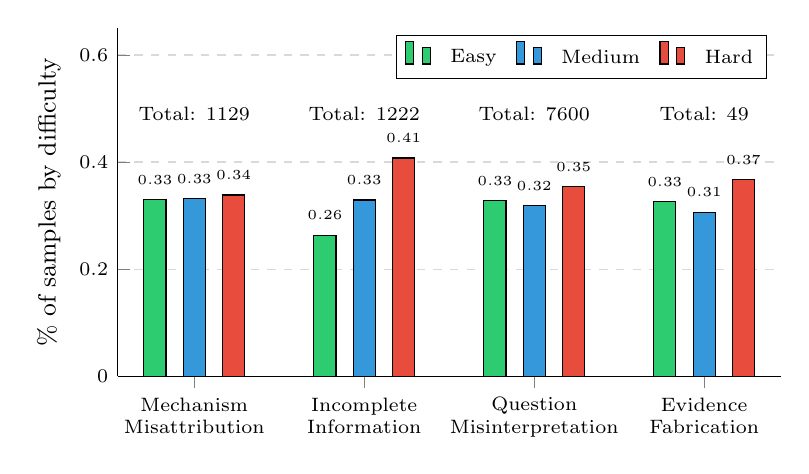
\begin{tikzpicture}[font=\small]
    % Define common colors
    \definecolor{easycolor}{RGB}{46,204,113}
    \definecolor{mediumcolor}{RGB}{52,152,219}
    \definecolor{hardcolor}{RGB}{231,76,60}
    
    \begin{axis}[
        width=10cm,
        height=6cm,
        ybar,
        bar width=8pt,
        ymin=0, ymax=0.65,
        ylabel={\% of samples by difficulty},
        symbolic x coords={MPM, II, MQ, MEF},
        xtick=data,
        xticklabels={
            {Mechanism\\Misattribution},
            {Incomplete\\Information},
            {Question\\Misinterpretation},
            {Evidence\\Fabrication}
        },
        x tick label style={align=center, font=\scriptsize},
        y tick label style={font=\scriptsize},
        legend style={
            at={(0.98,0.98)},
            anchor=north east,
            font=\scriptsize,
            legend columns=-1,
            transpose legend,
            row sep=0pt,
            column sep=5pt
        },
        ymajorgrids=true,
        grid style={dashed, gray!30},
        nodes near coords,
        every node near coord/.append style={
            anchor=south,
            font=\tiny,
            yshift=2pt
        },
        enlarge x limits=0.15,
        axis lines*=left  % This is the key change - only shows left axes
    ]
        \addplot[fill=easycolor, bar shift=-0.5cm] coordinates {
            (MPM, 0.3295) (II, 0.2635) (MQ, 0.3276) (MEF, 0.3265)
        };
        \addplot[fill=mediumcolor, bar shift= 0.00cm] coordinates {
            (MPM, 0.3322) (II, 0.3290) (MQ, 0.3182) (MEF, 0.3061)
        };
        \addplot[fill=hardcolor, bar shift= 0.5cm] coordinates {
            (MPM, 0.3384) (II, 0.4075) (MQ, 0.3542) (MEF, 0.3673)
        };
        \legend{Easy, Medium, Hard}
        
        \node[anchor=south] at (axis cs: MPM, 0.46) {\scriptsize Total: 1129};
        \node[anchor=south] at (axis cs: II, 0.46) {\scriptsize Total: 1222};
        \node[anchor=south] at (axis cs: MQ, 0.46) {\scriptsize Total: 7600};
        \node[anchor=south] at (axis cs: MEF, 0.46) {\scriptsize Total: 49};
        
    \end{axis}
\end{tikzpicture}
\end{document}
    }
    \caption{Statistics of the MedHallu dataset categorized by four categories of hallucinations (see Table \ref{tab:medical_hallucination_types} for detailed definitions) and levels of difficulty (easy, medium, hard).}
    \label{fig:statistics}
\end{figure}
% \textcolor{red}{TL: please show the specific statistics of generated datasets.}
\vspace{-2mm}

\subsection*{Dataset Generation Pipeline}
\vspace{-2mm}
The proposed methodological framework comprises a three-phase pipeline architected for robust hallucinated sample generation (Figure~\ref{fig:pipeline}). 
The pipeline follows a sequential approach: (1) stochastic sampling of potential hallucinated responses based on in-context examples and precise definitions, (2) LLM-based quality filtering mechanisms, (3) correctness checking using bidirectional entailment and LLM prompting. (4) Sequential Improvement via TextGrad. Finally, inspired by~\citep{Hallueval}, we select the most similar sample generated, using semantic similarity in cases where a high-quality sample is not identified. This approach enables comprehensive identification and evaluation of linguistic hallucinations while minimizing false positives through multi-layered verification protocols.

\begin{algorithm}[ht!]
\caption{\textit{NovelSelect}}
\label{alg:novelselect}
\begin{algorithmic}[1]
\State \textbf{Input:} Data pool $\mathcal{X}^{all}$, data budget $n$
\State Initialize an empty dataset, $\mathcal{X} \gets \emptyset$
\While{$|\mathcal{X}| < n$}
    \State $x^{new} \gets \arg\max_{x \in \mathcal{X}^{all}} v(x)$
    \State $\mathcal{X} \gets \mathcal{X} \cup \{x^{new}\}$
    \State $\mathcal{X}^{all} \gets \mathcal{X}^{all} \setminus \{x^{new}\}$
\EndWhile
\State \textbf{return} $\mathcal{X}$
\end{algorithmic}
\end{algorithm}


\paragraph{1) Diverse Hallucinated Answer Sampling.} \label{Sampling step}

Using a carefully crafted prompting strategy shown in Figure~\ref{fig:pipeline}, we generate multiple possible hallucinated answers with diverse temperature settings, we describe the prompt in Table~\ref{fig:system_prompt}. Through experiments, we find that allowing the model to choose the category of hallucination to apply to a given medical question performs better than manually forcing a specific hallucination category. For this generation $H_i = LM_i(Q_i,GT_i,C_i)$, we provide the LLM with precise definitions of each category, along with examples, question $Q_i$, and ground truth answers $GT_i$. The LLM is tasked with generating an answer that is semantically similar to ground truth yet incorrect. Additionally, we provide the ground truth context $C_i$, which contains precise knowledge required to answer the question. This includes intricate details necessary for crafting a strong hallucinated answer. 

\paragraph{2) Quality checking - LLM-based Discriminative Filtering.} \label{Quality check}

The second phase of our pipeline implements a comprehensive quality filtering protocol leveraging an ensemble of LLMs to minimize individual model biases. For each generated sample $H_i$, we employ a comparative assessment framework where multiple LLMs independently evaluate two candidate responses: the potentially hallucinated answer and the established ground truth. The quality assessment task is formulated as a binary classification problem, where models are prompted to identify which response appears more factually accurate given the question without access to the ground truth context. To mitigate potential biases from any single model, we implement a majority voting mechanism across different LLM architectures (including Gemma2, GPT-4o-mini, and Qwen2.5). A generated sample $H_i$ is preserved only when at least a majority of models in the ensemble incorrectly identify it as the more accurate response compared to the ground truth.
The difficulty categorization of generated samples is determined by the voting patterns across the LLM ensemble. Specifically, we classify $H_i$ as ``hard'' when all LLMs in the ensemble incorrectly identify it as accurate response, ``medium'' when multiple but not all LLMs are deceived, and ``easy'' when only a single LLM fails to identify the hallucination. This multi-model consensus approach helps ensure that preserved hallucinated samples are sufficiently convincing while reducing the impact of model-specific quirks or biases in the filtering process.
\vspace{-1mm}
\paragraph*{3) Correctness Checking via Entailment.} \label{Correctness check}
We implement a two-stage correctness verification protocol to ensure that the generated hallucinations are semantically distinct from the ground truth while maintaining coherence. First, we employ bidirectional entailment checking using a fine-tuned RoBERTa-large-MNLI model to quantify the semantic divergence between the hallucinated sample $H_i$ and ground truth $GT_i$. The bidirectional entailment score $\mathcal{E}$ is computed as:
$$\mathcal{E}(H_i, GT_i) = \min(\text{NLI}(H_i \rightarrow GT_i), \text{NLI}(GT_i \rightarrow H_i))$$

where $\text{NLI}(x \rightarrow y)$ represents the natural language inference score indicating whether $x$ entails $y$. We establish a stringent threshold $\tau$ and only retain samples that satisfy: $\mathcal{E}(H_i, GT_i) < \tau$. This ensures the hallucinated samples maintain sufficient semantic distance from the ground truth, minimizing false positives while requiring minimal human intervention.


\paragraph*{4) Sequential Improvement via TextGrad.} \label{improvement}
Our framework implements an iterative optimization step to enhance the quality of generated hallucinations that fail initial quality or correctness checks. When a generated sample $H_i$ fails to meet the established quality tests described in Section~\ref{Quality check}, we employ TextGrad optimization to refine subsequent generations through a feedback loop. The optimization process is formalized as: $H_{i+1} = \text{TextGrad}(H_i, F(H_i))$ where $F(H_i)$ represents feedback from the TextGrad optimizer, initialized with GPT-4o-mini. This refinement process (detailed in Section~\ref{Sampling step}) iterates up to five times, terminating either upon reaching a quality-compliant sample or exhausting the iteration limit. For each failed generation, TextGrad analyzes LLM feedback to identify hallucination indicators that make $H_i$ easily detectable. The feedback mechanism specifically focuses on two aspects: (1) linguistic patterns that signal artificial content and (2) structural elements that could be refined to enhance the naturalness. This feedback is then incorporated into subsequent prompt refinement, systematically improving both the content plausibility and stylistic cohesion. If no sample passes the quality filter after maximum iterations, we implement a fallback strategy based on semantic dissimilarity. Specifically, we select the candidate $H_*$ that maximizes the cosine similarity from the ground truth embedding: $H_* = \arg\max_{H_i} (\cos(\text{embed}(H_i), \text{embed}(GT_i)))$. This ensures that even in challenging cases, our pipeline produces outputs with maximum semantic similarity while preserving response coherence.

% \subsection*{Statistics about the MedHallu Dataset}




% \begin{table*}
% \centering
% \small
% \setlength{\tabcolsep}{4pt} % Reduce space between columns
% \begin{tabular}{l|ccccc|ccccc|c}
% \hline
% \textbf{Model} & \multicolumn{5}{c|}{Without Knowledge} & \multicolumn{5}{c|}{With Knowledge} & \textbf{$\Delta$ Know.} \\
% \hline
%               & \shortstack{Overall\\F1} & \shortstack{Overall\\P} & \shortstack{Easy\\F1} & \shortstack{Med\\F1} & \shortstack{Hard\\F1} 
%               & \shortstack{Overall\\F1} & \shortstack{Overall\\P} & \shortstack{Easy\\F1} & \shortstack{Med\\F1} & \shortstack{Hard\\F1} & \\
% \hline
% Qwen2.5-14B-Instruct   & 0.59 & 0.73 & 0.81 & 0.64 & 0.46 & \textbf{0.83} & 0.84 & \textbf{0.93} & 0.89 & 0.74 & +0.24 \\
% Gemma-2-9b-it        & 0.61 & 0.73 & \textbf{0.83} & \textbf{0.73} & 0.44 & 0.81 & 0.78 & 0.88 & 0.85 & \textbf{0.76} & +0.20 \\
% Llama-3.1-8B-Instruct  & 0.44 & \textbf{0.85} & 0.73 & 0.58 & 0.19 & 0.79 & \textbf{0.89} & 0.90 & 0.84 & 0.70 & \textbf{+0.35} \\
% Qwen2.5-7B-Instruct    & 0.51 & 0.73 & 0.78 & 0.58 & 0.31 & 0.81 & 0.85 & 0.92 & 0.83 & 0.74 & +0.30 \\
% Qwen2.5-3B-Instruct    & \textbf{0.62} & 0.47 & 0.66 & 0.67 & \textbf{0.57} & 0.66 & 0.50 & 0.69 & 0.65 & 0.66 & +0.04 \\
% GPT-4o-mini            & 0.55 & 0.78 & 0.81 & 0.65 & 0.35 & \textbf{0.83} & 0.84 & 0.90 & \textbf{0.91} & \textbf{0.76} & +0.28 \\
% DeepSeek-R1-Distill-Llama-8B & 0.51 & 0.61 & 0.64 & 0.62 & 0.40 & 0.77 & 0.83 & 0.87 & 0.80 & 0.69 & +0.26 \\
% \hline
% \textbf{Average (Pre-trained)} & 0.55 & 0.70 & 0.75 & 0.64 & 0.39 & 0.79 & 0.79 & 0.87 & 0.82 & 0.72 & +0.24 \\
% \hline
% \\[-1ex] % extra space before the next header
% \multicolumn{12}{l}{\textbf{Medical Fine-Tuned LLMs}} \\[1ex] % extra space after the header
% \hline
% OpenBioLLM-Llama3-8B & 0.58 & 0.55 & 0.61 & 0.58 & 0.56 & 0.56 & 0.56 & 0.55 & 0.56 & 0.56 & -0.02 \\
% BioMistral-7B       & 0.56 & 0.50 & 0.55 & 0.57 & 0.56 & 0.63 & 0.54 & 0.61 & 0.68 & 0.63 & +0.07 \\
% Llama-3.1-8B-UltraMedical & 0.58 & 0.58 & 0.76 & 0.65 & 0.45 & 0.70 & 0.73 & 0.79 & 0.71 & 0.65 & +0.12 \\
% \hline
% \textbf{Average (Fine-Tuned)} & 0.57 & 0.54 & 0.64 & 0.60 & 0.52 & 0.63 & 0.61 & 0.65 & 0.65 & 0.61 & +0.06 \\
% \hline
% \end{tabular}

% \caption{Performance comparison of different LLMs with and without knowledge. General pre-trained LLMs perform better than Medically fine-tuned LLMs in the task of Medical Hallucination, in terms of almost all metrics. P denotes, Precision. $\Delta$ Know is the performance change in Overall F1 when knowledge is provided to the LLM.}
% \label{tab:llm_performance_merged}
% \end{table*}



\begin{table*}[t]
    \centering
    % Reduce font size globally for this table
    % \scriptsize
    % Adjust row spacing if needed
    \renewcommand{\arraystretch}{1.2}
    % Scale the entire tabular environment to fit within \linewidth
    \begin{adjustbox}{width=1\linewidth, center}
    \begin{tabular}{lccccc|ccccc|c}
    \toprule
    \textbf{Model} & \multicolumn{5}{c|}{\textbf{Without Knowledge}} & \multicolumn{5}{c|}{\textbf{With Knowledge}} & \textbf{$\Delta$ Knowledge} \\
    \cmidrule(lr){1-6} \cmidrule(lr){7-11}
    \textbf{General LLMs} & \textbf{Overall F1} & \textbf{Overall P} & \textbf{Easy F1} & \textbf{Med F1} & \textbf{Hard F1} 
                   & \textbf{Overall F1} & \textbf{Overall P} & \textbf{Easy F1} & \textbf{Med F1} & \textbf{Hard F1} & ($\Delta$ F1)\\
    \cmidrule(lr){2-6} \cmidrule(lr){7-12}
    GPT-4o$^*$                       & \textbf{0.737} & 0.723 & \textbf{0.844} & \textbf{0.758} & \textbf{0.625} & \textbf{0.877} & \textbf{0.882} & \textbf{0.947} & \textbf{0.880} & \textbf{0.811} & 0.140 \\
    GPT-4o mini                  & 0.607 & 0.772 & 0.783 & 0.603 & 0.446 & 0.841 & 0.820 & 0.914 & 0.854 & 0.761 & 0.234 \\
    Qwen2.5-14B-Instruct         & 0.619 & 0.691 & 0.773 & 0.611 & 0.483 & 0.852 & 0.857 & 0.935 & 0.856 & 0.769 & 0.233 \\
    Gemma-2-9b-Instruct          & 0.515 & 0.740 & 0.693 & 0.512 & 0.347 & 0.838 & 0.809 & 0.918 & 0.848 & 0.758 & \textbf{0.323} \\
    Llama-3.1-8B-Instruct        & 0.522 & \textbf{0.791} & 0.679 & 0.515 & 0.372 & 0.797 & 0.775 & 0.880 & 0.796 & 0.722 & 0.275 \\
    DeepSeek-R1-Distill-Llama-8B & 0.514 & 0.570 & 0.589 & 0.515 & 0.444 & 0.812 & 0.864 & 0.895 & 0.794 & 0.751 & 0.298 \\
    Qwen2.5-7B-Instruct          & 0.553 & 0.745 & 0.733 & 0.528 & 0.402 & 0.839 & 0.866 & 0.923 & 0.832 & 0.770 & 0.286 \\
    Qwen2.5-3B-Instruct          & 0.606 & 0.495 & 0.667 & 0.602 & 0.556 &  0.676 & 0.514 & 0.693 & 0.677 & 0.661 & 0.070 \\
    Llama-3.2-3B-Instruct                  & 0.499 & 0.696 & 0.651 & 0.467 & 0.384 & 0.734 & 0.775 & 0.822 & 0.723 & 0.664 & 0.235 \\
    Gemma-2-2b-Instruct                   & 0.553 & 0.620 & 0.680 & 0.524 & 0.457 & 0.715 & 0.786 & 0.812 & 0.705 & 0.631 & 0.162 \\
    
    \midrule
    
    % \multicolumn{12}{l}{\textbf{Medical Fine-Tuned LLMs}} 
    \textbf{Medical Fine-Tuned LLMs} & \textbf{Overall F1} & \textbf{Overall P} & \textbf{Easy F1} & \textbf{Med F1} & \textbf{Hard F1} 
                   & \textbf{Overall F1} & \textbf{Overall P} & \textbf{Easy F1} & \textbf{Med F1} & \textbf{Hard F1} & {($\Delta$ F1)}\\
    \cmidrule(lr){2-6} \cmidrule(lr){7-12}
    OpenBioLLM-Llama3-8B         & 0.484 & 0.490 & 0.494 & 0.474 & 0.483 & 0.424 & 0.567 & 0.438 & 0.412 & 0.423 & -0.060 \\
    BioMistral-7B                & 0.570 & 0.518 & 0.627 & 0.563 & \textbf{0.525} & 0.648 & 0.516 & 0.652 & 0.660 & 0.634 & 0.078 \\
    Llama-3.1-8B-UltraMedical    & \textbf{0.619} & 0.657 & \textbf{0.747} & \textbf{0.596} & 0.524 & 0.773 & 0.679 & 0.832 & 0.777 & \textbf{0.718} & 0.153 \\
    Llama3-Med42-8B & 0.416 & \textbf{0.829} & 0.600 & 0.379 & 0.264 & \textbf{0.797} & \textbf{0.856} & \textbf{0.898} & \textbf{0.794} & 0.707 & \textbf{0.381} \\
    \midrule
    \textbf{Average (General LLMs, w/o GPT-4o)} 
                                 & \textbf{0.533} & \textbf{0.686} & \textbf{0.674} & \textbf{0.517} & 0.412 
                                 & \textbf{0.784} & \textbf{0.789} & \textbf{0.864} & \textbf{0.781} & \textbf{0.716} 
                                 & \textbf{0.251} \\
    \textbf{Average (Medical Fine-Tuned LLMs)} 
                                 & 0.522 & 0.623 & 0.617 & 0.503 & \textbf{0.449} 
                                 & 0.660 & 0.654 & 0.705 & 0.660 & 0.620 
                                 & 0.138 \\
    \bottomrule
    \end{tabular}
    \end{adjustbox}
    \caption{Performance comparison of different LLMs with and without knowledge on MedHallu (10,000 samples). General LLMs perform better than medically fine-tuned LLMs in the task of Medical Hallucination across most metrics. “Overall P” denotes precision, and “\(\Delta\) Knowledge” is the performance change in overall F1 when knowledge is provided. $^*$We exclude GPT-4o while calculating the average to have a fair comparison of model sizes for general vs. fine-tuned LLMs. Additional experimental details can be found in Appendix \ref{Gen_robust_check}.}
    \label{tab:llm_performance_merged}
\end{table*}
\vspace{-2.5mm}
\section{Implementation Details}
\vspace{-2.5mm}
% \paragraph{MedHallu Dataset Generation.} Generating hallucinated responses that preserve semantic alignment with the ground truth while subtly modifying it to outcompete discriminator models is a nuanced challenge.
\paragraph{MedHallu Dataset Generation Settings.} We generate hallucinated responses using \texttt{Qwen2.5B-14B}~\citep{qwen2025qwen25technicalreport}. The ground truth question-answer pairs are sourced from the \texttt{pqa\_labeled} split of PubMedQA~\citep{PubmedQA}, which contains 1,000 expert-annotated samples, supplemented with 9,000 instances randomly selected from the \texttt{pqa\_artificial} split. To achieve high-quality generation with adequate diversity, we utilize regulated sampling settings. The \texttt{temperature} is varied between 0.3 and 0.7, while the \texttt{nucleus sampling threshold (top-p)} is fixed at 0.95. These settings balance cohesion and variability. The maximum response length is capped at 512 tokens to ensure completeness while mitigating computational costs. Each hallucinated answer is limited to within ±10\% of its corresponding ground truth answer's length, ensuring uniform information density.

\noindent $\triangleright$ \textit{Quality \& correctness check.} For quality check, We employ three LLMs: \texttt{GPT-4o mini}~\citep{openai2024gpt4ocard}, \texttt{Gemma2-9B}~\citep{gemmateam2024gemma2improvingopen}, and \texttt{Qwen2.5-7B}~\citep{qwen2025qwen25technicalreport}. A response is retained only if it deceives at least one of these models (see Section~\ref{Quality check}). For \textit{correctness check,} we employ the \texttt{microsoft/deberta-large-mnli} model~\citep{he2021debertadecodingenhancedbertdisentangled},  applying bidirectional entailment with a confidence threshold of 0.75. 

\noindent $\triangleright$ \textit{TextGrad \& Fallback.} We integrate \texttt{TextGrad}~\cite{yuksekgonul2024textgradautomaticdifferentiationtext} with \texttt{GPT-4o mini} as the backend model to generate feedback for samples that fail either the quality or correctness checks. Each sample undergoes a maximum of five generation attempts. If no valid response is produced within these iterations, we adopt a \textbf{fallback strategy}, selecting the most semantically similar generated answer to the ground truth response.

\paragraph{Discriminator Model Settings.} We evaluate a diverse set of model architectures under two distinct settings: (1) \textbf{zero-shot} (without additional knowledge) and (2) \textbf{context-aware} (with ground truth context provision). The detection prompt is described in Figure~\ref{fig:system_prompt_for_detection}. This dual-setting approach allows us to assess both the baseline detection capabilities and the models' ability to leverage contextual information for improved discrimination. We examine both general-purpose and specialized medical models. The \textbf{general models} include \texttt{Gemma-2 (2B, 9B) Instruct}~\citep{gemmateam2024gemma2improvingopen}, \texttt{Llama-3.1 (3B, 8B) Instruct}~\citep{grattafiori2024llama3herdmodels}, \texttt{Qwen-2.5 (3B, 7B, 14B)}~\citep{qwen2025qwen25technicalreport}, \texttt{DeepSeek-R1-Llama 8B}~\citep{deepseekai2025deepseekr1incentivizingreasoningcapability}, \texttt{GPT-4o}, and \texttt{GPT-4o mini}~\citep{openai2024gpt4ocard}. Additionally, we evaluate four \textbf{fine-tuned medical LLMs} such as \texttt{OpenBioLLM-8B}~\citep{OpenBioLLMs}, \texttt{Llama3-Med42-8B}~\citep{christophe2024med42v2suiteclinicalllms}, \texttt{BioMistral-7B}~\citep{labrak2024biomistral}, and \texttt{UltraMedical}~\citep{zhang2024ultramedical} to compare domain-specific adaptations against general-purpose models. In this discriminative task, we maintain a temperature of approximately \texttt{0.2-0.3} for all models. For OpenAI models, we use the official API, while for open-weight models like Llama, Gemma, and Qwen, we utilize the \texttt{Hugging Face Pipeline} to ensure a consistent inference framework across all models.

% \paragraph{Hyperparameter Selection.} \jiawei{I prefer not to have a separate section for hyperparameter selection. We should incorporate it into the two paragraphs above.} To achieve high generation quality with adequate diversity, we utilize regulated sampling settings. The temperature is varied between 0.3 and 0.7, keeping a constant nucleus sampling threshold (top-p) of 0.95. These parameters are empirically optimized to balance between cohesion and variability in responses. For efficiency, the maximum generation length is limited to 512 tokens, ensuring complete responses without undue computational burden. Our experimental design incorporates several model access frameworks for a thorough evaluation. For OpenAI models, we utilize the official API, whereas for open-weight models like Llama, Gemma, and Qwen, we use the Hugging Face Pipeline to maintain uniform inference procedures across all models. To maintain quality control and consistency, we impose certain constraints on generated responses. Each hallucinated answer response must be approximately the same length as its ground truth answer, with a tolerance of ±10\%, to maintain similar information density. Moreover, our generation process is limited to a maximum of 5 attempts per question. If no appropriate response is found within this threshold that passes the quality and correctness check, we switch to our fallback strategy which relies on semantic similarity, as explained in Section~\ref{improvement}.

\section{Results and Analysis} \label{ResultsAnalysis}

% \textcolor{red}{TL: Structurize your results by bullets, and also let the detailed can directly reflect your conclusions.}

% \textcolor{red}{TL: the structure of the experiments part is poor. maybe consider to structure them into all studies related to detection, then generation, then extra research questions.}

% \kaidi{Do we need to compare our results with Med-Halt and/or HaluBench medical part to demonstrate we may have some conflict but reasonable results against theirs? }
\vspace{-2mm}
\subsection{Which language model performs the best at medical hallucination detection task?}

Our experimental results reveal significant variations in hallucination detection performance across model architectures in the zero-shot setting (without relevant knowledge provided). As presented in Table~\ref{tab:llm_performance_merged}, \ding{202}~the size of a model is not necessarily linked to its detection capabilities. For instance, \texttt{Qwen2.5-3B} achieves a high baseline overall F1 score (0.606), outperforming larger models such as \texttt{Gemma-9B} (0.515), \texttt{Llama-3.1-8B-Instruct} (0.522), and even the \texttt{Qwen2.5-7B} model (0.533). \ding{203}~All models exhibit notable performance degradation on ``hard'' samples, with even the best-performing models, such as \texttt{GPT-4o}, showing a significant F1 score drop and achieving only 0.625 in these challenging cases. \ding{204}~An intriguing observation is that, overall, general LLMs outperform medical fine-tuned LLMs in terms of precision and F1 scores in the easy and medium categories when no additional knowledge is provided.

% \section{Ablation Experiments}

% \kaidi{The findings here are more interesting and should be highlighted as xxx-level analysis or other things rather than ablation. We should emphasize only our benchmark can provide such information  }
% We perform an extensive ablation study on the generated samples by measuring performance gains by explicitly providing ground-truth context in the in-context prompt; we note a substantial performance gain in the detection capabilities across LLMs. Yet, the performances of powerful LLMs like Qwen-2.5 14B and Llama-3.1 8B stay in the low 80\%, showing significant scope for performance improvement. We also perform ablation on the generation samples by clustering them. Specifically, we generate 50 possible hallucinated answers for a given question and then cluster them using the bidirectional entailment method proposed in \citep{Farquhar2024DetectingHI_semantic_entropy}. We find that most clusters contain points that either all pass the quality check, leading to high-quality sentences, or all fail the quality check. This highly indicates that these clusters of meaning directly correlate to the quality of the hallucinated sample. Also, across all clusters, we find that the clusters that successfully pass the quality check are closer (measured using Euclidean distance) to the ground truth compared to those with samples that fail the quality check. Similar insights can be derived from other metrics like cosine similarity and rouge score, indicating that cluster meanings and their similarity with ground truth highly affect the quality of hallucination samples generated.
\vspace{-1mm}
\subsection{How does providing knowledge impact detection performance?}
Providing knowledge to the LLMs in this hallucination detection task, yields substantial and consistent improvements in hallucination detection across all evaluated LLM architectures. As shown in Table \ref{tab:llm_performance_merged}, \ding{202} every model benefits from the inclusion of knowledge. In general LLMs, the average overall F1 score increases from 0.533 (without knowledge) to 0.784 (with knowledge), corresponding to a gain of +0.251. In contrast, medically fine-tuned LLMs exhibit a much smaller improvement—from an average overall F1 of 0.522 to 0.660 (+0.138), likely because these models already incorporate specialized domain knowledge during training. Moreover, the scale of the model is pivotal for its performance. \ding{203} Larger structures, such as \texttt{Qwen2.5-14B}, reach an impressive overall F1 score of 0.852 when supplemented with domain knowledge, indicating that their increased capacity supports better text comprehension and integration of knowledge. In contrast, smaller models like \texttt{Qwen2.5-3B} experience just slight enhancement (+0.07 F1, from 0.606 to 0.676), underscoring the variability in how different model sizes effectively use additional information. Remarkably, \texttt{Gemma-2-9B} showed the most significant benefit from knowledge, with its overall F1 score rising from 0.515 to 0.838 (+0.323). Overall, these findings affirm the hypothesis that domain knowledge access improves an LLM's hallucination detection ability, while also emphasizing that both model scale and whether the model has been fine-tuned on medical data are critical to the extent of performance improvements.

% \begin{table}[h]
\footnotesize  % Make the table smaller
\centering
\setlength{\tabcolsep}{4pt}  % Reduce column spacing
\begin{tabular}{l|c|ccc|c}
\hline
\textbf{Model} & \textbf{Overall} & \textbf{Easy} & \textbf{Med} & \textbf{Hard} & $\Delta$ \\
& \textbf{F1} & \textbf{F1} & \textbf{F1} & \textbf{F1} & \textbf{F1} \\
\hline
GPT-4o mini & \textbf{0.83} & 0.94 & 0.85 & 0.76 & +0.26 \\
Qwen2.5-14B & 0.84 & 0.91 & 0.90 & 0.77 & +0.26 \\
Gemma-9B & 0.82 & 0.92 & 0.87 & 0.76 & +0.23 \\
Qwen2.5-7B & 0.81 & 0.89 & 0.85 & 0.74 & +0.29 \\
Gemma-2B & 0.63 & 0.72 & 0.65 & 0.58 & +0.21 \\
Llama-3.1-8B & 0.79 & 0.89 & 0.82 & 0.73 & +0.35 \\
Llama-3.2-3B & 0.64 & 0.72 & 0.71 & 0.56 & +0.28 \\
Qwen2.5-3B & 0.67 & 0.69 & 0.69 & 0.65 & +0.02 \\
\hline
\end{tabular}
\caption{Performance of LLMs with knowledge. $\Delta$ F1 shows the absolute improvement in Overall F1 score compared to no-knowledge setting. Models are sorted by overall F1 score.}
\label{tab:llm_performance_with_2}
\end{table}


\begin{table}
\centering
\small
\begin{tabular}{lccc}
\hline
\textbf{Metric} & \textbf{Mean} & \textbf{Mean} & \textbf{P-value} \\
 & \textbf{(fooled)} & \textbf{(not fooled)} & \\
\hline
Cosine similarity & 0.715 & 0.696 & 0.004 \\
Euclidean distance & 0.714 & 0.750 & 0.002 \\
Rouge1-F1 & 0.358 & 0.319 & 0.002 \\
\hline
\end{tabular}
\caption{The average similarity between the clusters generated in Section \ref{semantic_analysis} and the ground truth samples. Clusters containing samples that fool detection LLMs (i.e., hallucinations that are more challenging to detect) are notably closer to the ground truth.}
\label{tab:metrics_cluster}
\end{table}

\subsection{Semantic analysis of hallucinated and ground truth sentences.} \label{semantic_analysis}
% \jiawei{I feel like this section is different from the previous or later sections. This section is more related to the hallucination generation part. We may need to move this to section 3, as the robust check of our data generation pipeline?}
\vspace{-1mm}
To analyze semantic patterns in hallucinated responses, we conduct a comprehensive clustering analysis on an expanded set of generations. Specifically, we generate 50 candidate hallucinated responses for each question from our sampling phase, as described in Section~\ref{Quality check}. We retain all 50 candidate hallucinated responses, including those that fail the quality or correctness checks, to capture the semantic distribution across both successful and unsuccessful hallucinated answers. Using bidirectional entailment with a threshold of 0.75, we cluster these 50 candidate hallucinated responses along with the ground truth response, forming distinct semantic clusters that represent different conceptual approaches to the same question. This clustering methodology, adapted from~\citep{Farquhar2024DetectingHI_semantic_entropy}, allows us to analyze the semantic structure of hallucinated responses relative to the ground truth, yielding three significant findings:

\paragraph{Cluster-level Detection Patterns.}
Our analysis uncovers a binary discrimination effect within semantic clusters. \ding{202} Specifically, hallucinated responses in the same cluster tend to exhibit near-uniform performance—either consistently passing LLM detection (being favored over the ground truth) or being uniformly flagged as hallucinations. This finding strongly indicates that semantic content, rather than merely surface-level linguistic features, plays a pivotal role in shaping the LLM's discrimination behavior.
\vspace{-1mm}
\paragraph{Cluster Proximity Analysis.}
\ding{203} We find that clusters containing samples that reliably fool detection LLMs (hallucinations that are harder to detect) are notably closer to the ground truth answer in semantic vector space. This closeness is quantified via Euclidean distance, with additional support from cosine similarity and ROUGE scores (Table~\ref{tab:metrics_cluster}). Such proximity suggests that well-crafted hallucinated responses strike a balance, they remain semantically similar enough to the ground truth while incorporating meaningful deviations.

\vspace{-1mm}
\paragraph{Ground Truth Isolation.}
A particularly significant finding is the distinct semantic isolation of ground truth responses from clusters of hallucinated outputs. Empirical evidence demonstrates that ground truth responses rarely, if ever, align within the semantic clusters formed by hallucinations. This clear separation validates the robustness of our generation pipeline, ensuring that hallucinated responses retain semantic distinctness from factual content while upholding contextual relevance.
\begin{table}[h]
\centering
\scriptsize
\begin{tabular}{@{}l c c c c c@{}}
\toprule
\textbf{Model} & \textbf{F1\textsubscript{NS}} & \textbf{P\textsubscript{NS}} & \textbf{F1\textsubscript{R}} & \textbf{P\textsubscript{R}} & \textbf{Response\%} \\ 
\midrule
GPT-4o-mini                     & 66.6  & 66.8 & 60.7 & 77.2 & 98.4   \\
Gemma-2-2b-it                  & 57.1  & 59.9 & 55.3 & 54.1 & 82.7   \\
Llama-3.2-3B-Instruct           & 58.1  & 68.7 & 49.9 & 63.3 & 85.9   \\
Qwen2.5-3B-Instruct             & 65.2  & 67.2 & 60.6 & 50.2 & 65.7   \\
BioMistral-7B                 & 56.5  & 50.5 & 57.0 & 51.3 & 99.2   \\
Qwen2.5-7B-Instruct             & 69.3  & \textbf{94.6} & 55.3 & 73.7 & 47.5   \\
OpenBioLLM-Llama3-8B            & 48.8  & 48.4 & 48.4 & 56.3 & 99.7   \\
Llama-3.1-8B-UltraMedical       & 58.5  & 49.1 & 61.9 & 56.4 & 69.7   \\
DeepSeek-R1-Llama-8B    & 66.0  & 56.9 & 51.4 & 61.7 & 98.1   \\
Llama-3.1-8B-Instruct           & 51.7  & 90.4 & 52.2 & \textbf{86.0} & 98.2   \\
Gemma-2-9b-it                  & 61.4  & 85.5 & 51.5 & 71.5 & 37.6   \\
Qwen2.5-14B-Instruct            & 76.2  & 82.9 & 61.9 & 76.5 & 27.9   \\
GPT-4o                         & \textbf{79.5}  & 79.6 & \textbf{73.7} & 72.4 & 33.9   \\
\bottomrule
\end{tabular}
\caption{F1\textsubscript{NS} and P\textsubscript{NS} (Precision) represent performance with the ``Not Sure'' option, while F1\textsubscript{R} and P\textsubscript{R} (Precision) represent performance when required to answer. Response\% represents the percentage of questions answered with ``Yes'' or ``No'' even when the ``Not Sure'' option is available.}
\label{tab:model-comparison}
\end{table}

\vspace{-5mm}
\subsection{Analysis of models' ability to decline to answer}
% We introduce a ``not sure'' category to the existing ``hallucinated'' and ``not hallucinated'' categories in our detection prompt \jiawei{something like 'Figure S1'} figure \ref{fig:system_prompt_for_detection}. The results (Table \ref{tab:model-comparison}) reveal clear patterns across model sizes and knowledge integration. When models are allowed to express uncertainty, they achieve higher precision but lower recall, effectively maintaining better F1 scores by avoiding low-confidence answers. Different model families show distinct characteristics in handling this trade-off, with Qwen models demonstrating the most consistent performance across both scenarios \jiawei{not true for 'Qwen2.5-14B-Instruct'} , while Llama models show greater variation. Larger models, particularly the 14B and 7B variants, excel in forced-answer scenarios, with Qwen-14B showing remarkable stability. Across both scenarios, knowledge-enabled models consistently outperform their counterparts. Interestingly, 
% \jiawei{What are 'these models?' knowledge-enabled models?} these models appear to use the ``not sure'' option more strategically. The performance gap between knowledge-enabled and knowledge-disabled versions widens when models are required to provide an answer.
% This suggests that enabling the ``not sure'' option benefits applications prioritizing precision, while those requiring higher coverage might benefit from forced answers. 

We introduce a ``not sure'' category alongside the existing ``hallucinated'' and ``not hallucinated'' categories in our detection prompt (Figure \ref{fig:system_prompt_for_detection}), allowing LLMs to decline to answer if they lack full confidence in their responses. Results shown in Table \ref{tab:model-comparison}, reveal that \ding{202} many models demonstrate an improved F1 score and precision when they can opt for ``not sure.'' However, the enhancement varies with model size: smaller models gain a moderate improvement of 3-5\%, whereas larger models see a significant boost of around 10-15\%. General LLMs outperform fine-tuned medical models, with some like GPT-4o achieving up to 79.5\% in performance, and Qwen2.5-14B performing closely at 76.2\%. \ding{203} In terms of the percentage of questions answered with definite ``yes'' or ``no'' (Response Rate), general LLMs respond to fewer questions, with Qwen2.5-14B responding to as little as 27.9\%, reflecting their tendency to skip uncertain questions. Conversely, fine-tuned medical models attempt to answer nearly all questions, rarely selecting the ``Not Sure'' option. This approach sometimes leads to a minor reduction in performance. For instance, UltraMedical's model has the lowest response rate among medical models at 69.7\% , while OpenBioLLM reaches as high as 99.7\%. Finally, \ding{204} when comparing the impact of adding the ``not sure'' choice with knowledge-sharing enhancements, shown in Table \ref{tab:model-comparison-with-knowledge} versus Table \ref{tab:model-comparison}, there is a marked increase in the percentage of questions attempted by General LLMs, suggesting improved confidence in task execution, along with an increase in F1 score and precision.

\begin{figure}
    \centering
    \tiny
    \resizebox{\columnwidth}{!}{
        %Draw graphics
\usepackage{pgfplots}
\usepackage{pgfplotstable}
\pgfplotsset{compat=newest}
\pgfplotscreateplotcyclelist{my chart colors}{%
blue, solid, every mark/.append style={solid, fill=blue}, mark=*\\%
red, solid, every mark/.append style={solid, fill=red}, mark=square*\\%
brown, solid, every mark/.append style={solid, fill=brown}, mark=triangle*\\%
cyan, solid, every mark/.append style={solid, fill=gray}, mark=diamond*\\%
black, dashdotted, every mark/.append style={solid, fill=red}, mark=halfdiamond*\\%
olive, dashdotted, every mark/.append style={solid, fill=green}, mark=halfcircle*\\%
orange, dashdotted, every mark/.append style={solid, fill=gray}, mark=*\\%
purple, dashdotted, every mark/.append style={solid, fill=blue}, mark=halfsquare left*\\%
teal, densely dashed, every mark/.append style={solid, fill=green}, mark=oplus*\\%
violet, densely dashed, every mark/.append style={solid, fill=gray}, mark=diamond*\\%
magenta, densely dashed, every mark/.append style={solid, fill=blue}, mark=triangle*\\%
lime, densely dashed, every mark/.append style={solid, fill=red}, mark=square*\\%
}

\newcommand{\errorband}[5][]{ % x column, y column, error column, optional argument for setting style of the area plot
\pgfplotstableread[col sep=comma, skip first n=2]{#2}\datatable
    % Lower bound (invisible plot)
    \addplot [draw=none, stack plots=y, forget plot] table [
        x={#3},
        y expr=\thisrow{#4}-\thisrow{#5}
    ] {\datatable};

    % Stack twice the error, draw as area plot
    \addplot [draw=none, fill=gray!40, stack plots=y, area legend, #1] table [
        x={#3},
        y expr=2*\thisrow{#5}
    ] {\datatable} \closedcycle;

    % Reset stack using invisible plot
    \addplot [forget plot, stack plots=y,draw=none] table [x={#3}, y expr=-(\thisrow{#4}+\thisrow{#5})] {\datatable};
}
    }
    \caption{Detection accuracy of different hallucination categories on MedHallu, evaluated using \texttt{Qwen2-7B-Instruct} as the discriminator.}
    \label{fig:hallucination_types}
\end{figure}

% \vspace{-9mm}
\subsection{Analysis: Hallucination category and MeSH}

\subsubsection*{Which hallucination category is hardest to detect? }
Our analysis reveals distinct patterns in detection difficulty across hallucination categories, as shown in Figure~\ref{fig:hallucination_types}. \textbf{Incomplete Information (II)} emerges as the most challenging category, with 41\% of total samples being ``hard'' cases (Figure \ref{fig:statistics}) and the lowest detection ratio (54\%), indicating models struggle significantly with validating partial information. \textbf{Mechanism/Pathway Misattribution (MPM)} and \textbf{Question Misinterpretation (MQ)} show notable patterns: MPM has a significant number of hard cases, with a 68\% detection accuracy, while MQ having higher number of hard cases but stronger detection performance (68.8\%). \textbf{Methodological and Evidence Fabrication (MEF)}, despite being the smallest category (37\% are hard), demonstrates the highest detection success rate (76.6\%).

\noindent These findings highlight a crucial insight: subtle manipulation of existing medical information, particularly through incomplete presentation, is harder to detect than outright fabrication. This is evident from II's high difficulty scores compared to MEF's better detection rates. The distribution across difficulty levels (easy, medium, hard) further supports this, with II showing the highest concentration in the ``hard'' category. This suggests that while models excel at identifying completely fabricated information, they struggle with partially accurate yet incomplete medical claims, highlighting critical areas of improvement in hallucination detection systems.

\subsubsection*{Which medical category (MeSH term) hallucination is the hardest to detect?}

\noindent To understand which medical domains are more susceptible to hallucination, we examine the MedHallu dataset with the MeSH categories within the PubMedQA dataset, identifying the top five principal categories shown in Figure~\ref{fig:mesh_categories}. These categories include Diseases (comprising 25.9\% of the samples), Analytical Procedures (20.1\%), Chemical/Drug Queries (15.8\%), Healthcare Management (9.7\%), and Psychiatric Conditions (6.7\%). Detection performance among these categories varies considerably: Disease-related instances exhibit a respectable detection accuracy of 57.1\%, despite the abundance of related medical literature in the corpus. Conversely, Chemical/Drug queries demonstrate the highest detection rate at 67.7\%. In contrast, Psychiatry ranks lowest among the top five categories with a detection rate of just 53.7\%, highlighting the need for further incorporation of this data in the training corpus.

\begin{figure}[t]
    \centering
    \tiny
    \scalebox{0.7}{
        \documentclass{standalone}
\usepackage{tikz}
\usepackage{pgfplots}
\pgfplotsset{compat=1.18}

\begin{document}
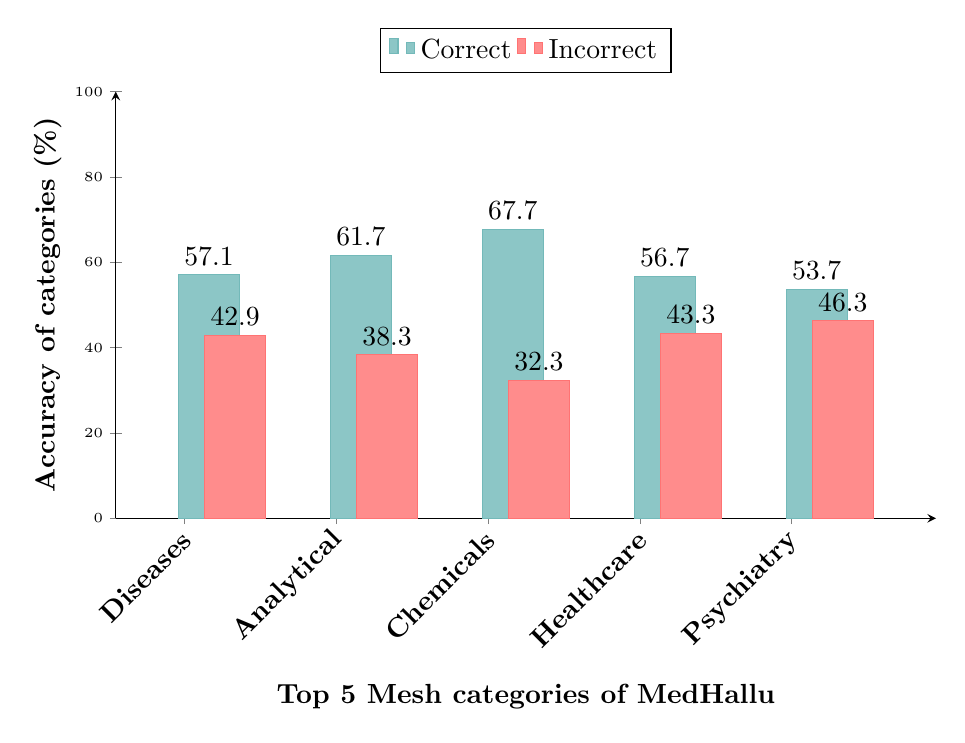
\begin{tikzpicture}
\tiny
\begin{axis}[
    width=12cm,
    height=7cm,
    ybar=-40pt,    % Reduced from 8pt to bring bars closer
    bar width=22pt,
    ylabel={\normalsize\textbf{Accuracy of categories (\%)}},
    xlabel={\normalsize\textbf{Top 5 Mesh categories of MedHallu}},
    xlabel style={yshift=-1em}, 
    symbolic x coords={D1,D2,A1,A2,C1,C2,H1,H2,P1,P2},
    xtick={D1,A1,C1,H1,P1},
    xticklabels={\normalsize\textbf{Diseases}, \normalsize\textbf{Analytical}, \normalsize\textbf{Chemicals}, \normalsize\textbf{Healthcare}, \normalsize\textbf{Psychiatry}},
    xticklabel style={
        rotate=45,           % Rotates labels 45 degrees
        anchor=east,         % Aligns the labels properly
        yshift=-0.5em        % Adjusts vertical position
    },
    legend style={
        at={(0.5,1.15)},
        anchor=north,
        legend columns=2,
        font=\normalsize
    },
    ymin=0,
    ymax=100,   % Changed to a percentage scale
    axis lines=left,
    clip=false,
    enlarge x limits=0.1,  % Reduced side margins
    nodes near coords,
    nodes near coords style={font=\normalsize},
    every node near coord/.append style={yshift=1pt}
]

% Calculated percentages (rounded to one decimal place):
% Diseases: Correct: 148/259*100 ≈ 57.1, Incorrect: 111/259*100 ≈ 42.9
% Analytical: Correct: 124/201*100 ≈ 61.7, Incorrect: 77/201*100 ≈ 38.3
% Chemicals: Correct: 107/158*100 ≈ 67.7, Incorrect: 51/158*100 ≈ 32.3
% Healthcare: Correct: 55/97*100 ≈ 56.7, Incorrect: 42/97*100 ≈ 43.3
% Psychiatry: Correct: 36/67*100 ≈ 53.7, Incorrect: 31/67*100 ≈ 46.3

\addplot[fill=teal!45!white, draw=teal!55!white] coordinates {
    (D1,57.1) (A1,61.7) (C1,67.7) (H1,56.7) (P1,53.7)
}; \addlegendentry{Correct}

\addplot[fill=red!45!white, draw=red!55!white] coordinates {
    (D2,42.9) (A2,38.3) (C2,32.3) (H2,43.3) (P2,46.3)
}; \addlegendentry{Incorrect}

\label{Mesh_class_plot}
\end{axis}
\end{tikzpicture}
\end{document}
    }
    \caption{Detection accuracy across Mesh categories proposed in PubMedQA. We use \texttt{Qwen2.5-7B-Instruct} as a discriminator for the 1k samples of MedHallu generated on pqa\_labeled split.}
    \label{fig:mesh_categories}
\end{figure}

\vspace{-2mm}
\section{Conclusion}
\vspace{-2mm}
We introduce MedHallu, a comprehensive benchmark comprising 10,000 rigorously curated medical question-answer pairs with hallucinated answers. MedHallu integrates fine-grained categorization of medical hallucination types, a hallucination generation framework that balances difficulty levels while mitigating single-LLM bias through multi-model majority voting, and systematically evaluates diverse LLM configurations' hallucination detection capabilities. Our evaluation reveals that existing LLMs exhibit significant limitations in detecting medical hallucinations, particularly struggling with "hard" hallucination answers, which are closer in distance to the ground truth. We also provide insights into enhancing LLMs' hallucination detection: when knowledge is provided, general-purpose LLMs can outperform medical fine-tuned models, and allowing models to decline to answer by providing a "not sure" option improves precision in critical applications. As the largest open medical hallucination benchmark to date, MedHallu serves as a valuable resource for evaluating LLMs' medical hallucination detection abilities and offers insights into the cautious use of LLMs in high-stakes medical domains.


\section{Limitations}
Our study faces three primary constraints. First, due to resource constraints, we could not employ the most advanced reasoning models (e.g., OpenAI o1, Gemini 2.0, DeepSeek-R1) for benchmark generation. While our pipeline incorporates multi-stage LLM quality checks and regeneration steps, using state-of-the-art models would incur prohibitive computational costs. Second, our evaluation of LLMs was restricted to input-output prompting (zero-shot, with/without knowledge provision); resource limitations precluded exploration of advanced techniques like chain-of-thought or self-consistency, which might better elicit model capabilities. Third, our hallucination generation pipeline relied on the PubMedQA corpus to ensure contextual fidelity. While this ensures biomedical relevance, future work should incorporate diverse high-quality corpora to improve scalability and domain coverage.

\section{Ethics Statement}
This research adheres to rigorous ethical standards in dataset creation and evaluation. The MedHallu benchmark utilizes publicly available PubMedQA data under MIT licenses, ensuring proper attribution and compliance with source terms of use. Patient privacy is preserved through the exclusive use of de-identified biomedical literature. While our work aims to improve AI safety in healthcare, we acknowledge potential dual-use risks and advocate for responsible deployment of medical LLMs with human oversight. The benchmark's stratification enables targeted mitigation of dangerous ``hard'' hallucinations that most closely resemble factual content. All artifacts will be released with detailed documentation to promote transparency and reproducibility in medical AI safety research.


% This work introduces MedHallu, a comprehensive benchmark for evaluating medical hallucination detection capabilities in large language models. Through our systematic evaluation of 50,000 question-answer pairs across various medical domains, we have uncovered several critical insights about the current state and limitations of hallucination detection in medical AI systems.
% Our findings demonstrate that even state-of-the-art language models struggle with medical hallucination detection, achieving only moderate performance in zero-shot settings (F1 scores of 0.65 or lower). The provision of ground truth context significantly improves detection capabilities across all models, with some achieving F1 scores up to 0.84, highlighting the crucial role of knowledge grounding in enhancing model reliability. However, the persistent challenges in detecting ``hard'' cases, particularly those involving incomplete information, underscore the complexity of this task and the need for continued advancement in model architectures and training approaches.

% The semantic clustering analysis revealed that hallucination detection is primarily influenced by semantic content rather than surface-level features, with clear patterns emerging in how models evaluate responses within similar semantic clusters. This finding suggests that future improvements in hallucination detection should focus on enhancing models' semantic understanding capabilities rather than purely syntactic features.

% These findings have significant implications for deploying AI systems in healthcare settings. The substantial improvement in detection performance, when models are provided with ground truth context (+35\% F1 score in some cases), suggests that future medical AI systems should be designed with robust knowledge integration capabilities. Additionally, the benefits of allowing models to express uncertainty (``not sure'' option) in improving precision highlights the importance of implementing appropriate confidence thresholds in clinical applications.

% As AI systems become increasingly integrated into healthcare decision-making processes, the ability to reliably detect and filter out hallucinated information becomes crucial. The MedHallu benchmark provides a foundation for evaluating and improving these capabilities, contributing to developing more reliable and trustworthy medical AI systems.

% \bibliographystyle{acl_natbib}
\bibliography{bib} 

\clearpage

\appendix

%\title{Generating 3D \hl{Small} Binding Molecules Using Shape-Conditioned Diffusion Models with Guidance}
%\date{\vspace{-5ex}}

%\author{
%	Ziqi Chen\textsuperscript{\rm 1}, 
%	Bo Peng\textsuperscript{\rm 1}, 
%	Tianhua Zhai\textsuperscript{\rm 2},
%	Xia Ning\textsuperscript{\rm 1,3,4 \Letter}
%}
%\newcommand{\Address}{
%	\textsuperscript{\rm 1}Computer Science and Engineering, The Ohio Sate University, Columbus, OH 43210.
%	\textsuperscript{\rm 2}Perelman School of Medicine, University of Pennsylvania, Philadelphia, PA 19104.
%	\textsuperscript{\rm 3}Translational Data Analytics Institute, The Ohio Sate University, Columbus, OH 43210.
%	\textsuperscript{\rm 4}Biomedical Informatics, The Ohio Sate University, Columbus, OH 43210.
%	\textsuperscript{\Letter}ning.104@osu.edu
%}

%\newcommand\affiliation[1]{%
%	\begingroup
%	\renewcommand\thefootnote{}\footnote{#1}%
%	\addtocounter{footnote}{-1}%
%	\endgroup
%}



\setcounter{secnumdepth}{2} %May be changed to 1 or 2 if section numbers are desired.

\setcounter{section}{0}
\renewcommand{\thesection}{S\arabic{section}}

\setcounter{table}{0}
\renewcommand{\thetable}{S\arabic{table}}

\setcounter{figure}{0}
\renewcommand{\thefigure}{S\arabic{figure}}

\setcounter{algorithm}{0}
\renewcommand{\thealgorithm}{S\arabic{algorithm}}

\setcounter{equation}{0}
\renewcommand{\theequation}{S\arabic{equation}}


\begin{center}
	\begin{minipage}{0.95\linewidth}
		\centering
		\LARGE 
	Generating 3D Binding Molecules Using Shape-Conditioned Diffusion Models with Guidance (Supplementary Information)
	\end{minipage}
\end{center}
\vspace{10pt}

%%%%%%%%%%%%%%%%%%%%%%%%%%%%%%%%%%%%%%%%%%%%%
\section{Parameters for Reproducibility}
\label{supp:experiments:parameters}
%%%%%%%%%%%%%%%%%%%%%%%%%%%%%%%%%%%%%%%%%%%%%

We implemented both \SE and \methoddiff using Python-3.7.16, PyTorch-1.11.0, PyTorch-scatter-2.0.9, Numpy-1.21.5, Scikit-learn-1.0.2.
%
We trained the models using a Tesla V100 GPU with 32GB memory and a CPU with 80GB memory on Red Hat Enterprise 7.7.
%
%We released the code, data, and the trained model at Google Drive~\footnote{\url{https://drive.google.com/drive/folders/146cpjuwenKGTd6Zh4sYBy-Wv6BMfGwe4?usp=sharing}} (will release to the public on github once the manuscript is accepted).

%===================================================================
\subsection{Parameters of \SE}
%===================================================================


In \SE, we tuned the dimension of all the hidden layers including VN-DGCNN layers
(Eq.~\ref{eqn:shape_embed}), MLP layers (Eq.~\ref{eqn:se:decoder}) and
VN-In layer (Eq.~\ref{eqn:se:decoder}), and the dimension $d_p$ of generated shape latent embeddings $\shapehiddenmat$ with the grid-search algorithm in the 
parameter space presented in Table~\ref{tbl:hyper_se}.
%
We determined the optimal hyper-parameters according to the mean squared errors of the predictions of signed distances for 1,000 validation molecules that are selected as described in Section ``Data'' 
in the main manuscript.
%
The optimal dimension of all the hidden layers is 256, and the optimal dimension $d_p$ of shape latent embedding \shapehiddenmat is 128.
%
The optimal number of points $|\pc|$ in the point cloud \pc is 512.
%
We sampled 1,024 query points in $\mathcal{Z}$ for each molecule shape.
%
We constructed graphs from point clouds, which are employed to learn $\shapehiddenmat$ with VN-DGCNN layer (Eq.~\ref{eqn:shape_embed}), using the $k$-nearest neighbors based on Euclidean distance with $k=20$.
%
We set the number of VN-DGCNN layers as 4.
%
We set the number of MLP layers in the decoder (Eq.~\ref{eqn:se:decoder}) as 2.
%
We set the number of VN-In layers as 1.

%
We optimized the \SE model via Adam~\cite{adam} with its parameters (0.950, 0.999), %betas (0.95, 0.999), 
learning rate 0.001, and batch size 16.
%
We evaluated the validation loss every 2,000 training steps.
%
We scheduled to decay the learning rate with a factor of 0.6 and a minimum learning rate of 1e-6 if 
the validation loss does not decrease in 5 consecutive evaluations.
%
The optimal \SE model has 28.3K learnable parameters. 
%
We trained the \SE model %for at most 80 hours 
with $\sim$156,000 training steps.
%
The training took 80 hours with our GPUs.
%
The trained \SE model achieved the minimum validation loss at 152,000 steps.


\begin{table*}[!h]
  \centering
      \caption{{Hyper-Parameter Space for \SE Optimization}}
  \label{tbl:hyper_se}
  \begin{threeparttable}
 \begin{scriptsize}
      \begin{tabular}{
%	@{\hspace{2pt}}l@{\hspace{2pt}}
	@{\hspace{2pt}}l@{\hspace{5pt}} 
	@{\hspace{2pt}}r@{\hspace{2pt}}         
	}
        \toprule
        %Notation &
          Hyper-parameters &  Space\\
        \midrule
        %$t_a$    & 
         %hidden layer dimension         & \{16, 32, 64, 128\} \\
         %atom/node embedding dimension &  \{16, 32, 64, 128\} \\
         %$\latent^{\add}$/$\latent^{\delete}$ dimension        & \{8, 16, 32, 64\} \\
         hidden layer dimension            & \{128, 256\}\\
         dimension $d_p$ of \shapehiddenmat        &  \{64, 128\} \\
         \#points in \pc        & \{512, 1,024\} \\
         \#query points in $\mathcal{Z}$                & 1,024 \\%1024 \\%\bo{\{1024\}}\\
         \#nearest neighbors              & 20          \\
         \#VN-DGCNN layers (Eq~\ref{eqn:shape_embed})               & 4            \\
         \#MLP layers in Eq~\ref{eqn:se:decoder} & 4           \\
        \bottomrule
      \end{tabular}
%  	\begin{tablenotes}[normal,flushleft]
%  		\begin{footnotesize}
%  	
%  	\item In this table, hidden dimension represents the dimension of hidden layers and 
%  	atom/node embeddings; latent dimension represents the dimension of latent embedding \latent.
%  	\par
%  \end{footnotesize}
%  
%\end{tablenotes}
%      \begin{tablenotes}
%      \item 
%      \par
%      \end{tablenotes}
\end{scriptsize}
  \end{threeparttable}
\end{table*}

%
\begin{table*}[!h]
  \centering
      \caption{{Hyper-Parameter Space for \methoddiff Optimization}}
  \label{tbl:hyper_diff}
  \begin{threeparttable}
 \begin{scriptsize}
      \begin{tabular}{
%	@{\hspace{2pt}}l@{\hspace{2pt}}
	@{\hspace{2pt}}l@{\hspace{5pt}} 
	@{\hspace{2pt}}r@{\hspace{2pt}}         
	}
        \toprule
        %Notation &
          Hyper-parameters &  Space\\
        \midrule
        %$t_a$    & 
         %hidden layer dimension         & \{16, 32, 64, 128\} \\
         %atom/node embedding dimension &  \{16, 32, 64, 128\} \\
         %$\latent^{\add}$/$\latent^{\delete}$ dimension        & \{8, 16, 32, 64\} \\
         scalar hidden layer dimension         & 128 \\
         vector hidden layer dimension         & 32 \\
         weight of atom type loss $\xi$ (Eq.~\ref{eqn:loss})  & 100           \\
         threshold of step weight $\delta$ (Eq.~\ref{eqn:diff:obj:pos}) & 10 \\
         \#atom features $K$                   & 15 \\
         \#layers $L$ in \molpred             & 8 \\
         %\# \eqgnn/\invgnn layers     &  8 \\
         %\# heads {$n_h$} in $\text{MHA}^{\mathtt{x}}/\text{MHA}^{\mathtt{v}}$                               & 16 \\
         \#nearest neighbors {$N$}  (Eq.~\ref{eqn:geometric_embedding} and \ref{eqn:attention})            & 8          \\
         {\#diffusion steps $T$}                  & 1,000 \\
        \bottomrule
      \end{tabular}
%  	\begin{tablenotes}[normal,flushleft]
%  		\begin{footnotesize}
%  	
%  	\item In this table, hidden dimension represents the dimension of hidden layers and 
%  	atom/node embeddings; latent dimension represents the dimension of latent embedding \latent.
%  	\par
%  \end{footnotesize}
%  
%\end{tablenotes}
%      \begin{tablenotes}
%      \item 
%      \par
%      \end{tablenotes}
\end{scriptsize}
  \end{threeparttable}

\end{table*}


%===================================================================
\subsection{Parameters of \methoddiff}
%===================================================================

Table~\ref{tbl:hyper_diff} presents the parameters used to train \methoddiff.
%
In \methoddiff, we set the hidden dimensions of all the MLP layers and the scalar hidden layers in GVPs (Eq.~\ref{eqn:pred:gvp} and Eq.~\ref{eqn:mess:gvp}) as 128. %, including all the MLP layers in \methoddiff and the scalar dimension of GVP layers in Eq.~\ref{eqn:pred:gvp} and Eq.~\ref{eqn:mess:gvp}. %, and MLP layer (Eq.~\ref{eqn:diff:graph:atompred}) as 128.
%
We set the dimensions of all the vector hidden layers in GVPs as 32.
%
We set the number of layers $L$ in \molpred as 8.
%and the number of layers in graph neural networks as 8.
%
Both two GVP modules in Eq.~\ref{eqn:pred:gvp} and Eq.~\ref{eqn:mess:gvp} consist of three GVP layers. %, which consisa GVP modset the number of layer of GVP modules %is a multi-head attention layer ($\text{MHA}^{\mathtt{x}}$ or $\text{MHA}^{\mathtt{h}}$) with 16 heads.
% 
We set the number of VN-MLP layers in Eq.~\ref{eqn:shaper} as 1 and the number of MLP layers as 2 for all the involved MLP functions.
%

We constructed graphs from atoms in molecules, which are employed to learn the scalar embeddings and vector embeddings for atoms %predict atom coordinates and features  
(Eq.~\ref{eqn:geometric_embedding} and \ref{eqn:attention}), using the $N$-nearest neighbors based on Euclidean distance with $N=8$. 
%
We used $K=15$ atom features in total, indicating the atom types and its aromaticity.
%
These atom features include 10 non-aromatic atoms (i.e., ``H'', ``C'', ``N'', ``O'', ``F'', ``P'', ``S'', ``Cl'', ``Br'', ``I''), 
and 5 aromatic atoms (i.e., ``C'', ``N'', ``O'', ``P'', ``S'').
%
We set the number of diffusion steps $T$ as 1,000.
%
We set the weight $\xi$ of atom type loss (Eq.~\ref{eqn:loss}) as $100$ to balance the values of atom type loss and atom coordinate loss.
%
We set the threshold $\delta$ (Eq.~\ref{eqn:diff:obj:pos}) as 10.
%
The parameters $\beta_t^{\mathtt{x}}$ and $\beta_t^{\mathtt{v}}$ of variance scheduling in the forward diffusion process of \methoddiff are discussed in 
Supplementary Section~\ref{supp:forward:variance}.
%
%Please note that as in \squid, we did not perform extensive hyperparameter optimization for \methoddiff.
%
Following \squid, we did not perform extensive hyperparameter tunning for \methoddiff given that the used 
hyperparameters have enabled good performance.

%
We optimized the \methoddiff model via Adam~\cite{adam} with its parameters (0.950, 0.999), learning rate 0.001, and batch size 32.
%
We evaluated the validation loss every 2,000 training steps.
%
We scheduled to decay the learning rate with a factor of 0.6 and a minimum learning rate of 1e-5 if 
the validation loss does not decrease in 10 consecutive evaluations.
%
The \methoddiff model has 7.8M learnable parameters. 
%
We trained the \methoddiff model %for at most 60 hours 
with $\sim$770,000 training steps.
%
The training took 70 hours with our GPUs.
%
The trained \methoddiff achieved the minimum validation loss at 758,000 steps.

During inference, %the sampling, 
following Adams and Coley~\cite{adams2023equivariant}, we set the variance $\phi$ 
of atom-centered Gaussians as 0.049, which is used to build a set of points for shape guidance in Section ``\method with Shape Guidance'' 
in the main manuscript.
%
We determined the number of atoms in the generated molecule using the atom number distribution of training molecules that have surface shape sizes similar to the condition molecule.
%
The optimal distance threshold $\gamma$ is 0.2, and the optimal stop step $S$ for shape guidance is 300.
%
With shape guidance, each time we updated the atom position (Eq.~\ref{eqn:shape_guidance}), we randomly sampled the weight $\sigma$ from $[0.2, 0.8]$. %\bo{(XXX)}.
%
Moreover, when using pocket guidance as mentioned in Section ``\method with Pocket Guidance'' in the main manuscript, each time we updated the atom position (Eq.~\ref{eqn:pocket_guidance}), we randomly sampled the weight $\epsilon$ from $[0, 0.5]$. 
%
For each condition molecule, it took around 40 seconds on average to generate 50 molecule candidates with our GPUs.



%%%%%%%%%%%%%%%%%%%%%%%%%%%%%%%%%%%%%%%%%%%%%%
\section{Performance of \decompdiff with Protein Pocket Prior}
\label{supp:app:decompdiff}
%%%%%%%%%%%%%%%%%%%%%%%%%%%%%%%%%%%%%%%%%%%%%%

In this section, we demonstrate that \decompdiff with protein pocket prior, referred to as \decompdiffbeta, shows very limited performance in generating drug-like and synthesizable molecules compared to all the other methods, including \methodwithpguide and \methodwithsandpguide.
%
We evaluate the performance of \decompdiffbeta in terms of binding affinities, drug-likeness, and diversity.
%
We compare \decompdiffbeta with \methodwithpguide and \methodwithsandpguide and report the results in Table~\ref{tbl:comparison_results_decompdiff}.
%
Note that the results of \methodwithpguide and \methodwithsandpguide here are consistent with those in Table~\ref{tbl:overall_results_docking2} in the main manuscript.
%
As shown in Table~\ref{tbl:comparison_results_decompdiff}, while \decompdiffbeta achieves high binding affinities in Vina M and Vina D, it substantially underperforms \methodwithpguide and \methodwithsandpguide in QED and SA.
%
Particularly, \decompdiffbeta shows a QED score of 0.36, while \methodwithpguide substantially outperforms \decompdiffbeta in QED (0.77) with 113.9\% improvement.
%
\decompdiffbeta also substantially underperforms \methodwithpguide in terms of SA scores (0.55 vs 0.76).
%
These results demonstrate the limited capacity of \decompdiffbeta in generating drug-like and synthesizable molecules.
%
As a result, the generated molecules from \decompdiffbeta can have considerably lower utility compared to other methods.
%
Considering these limitations of \decompdiffbeta, we exclude it from the baselines for comparison.

\begin{table*}[!h]
	\centering
		\caption{Comparison on PMG among \methodwithpguide, \methodwithsandpguide and \decompdiffbeta}
	\label{tbl:comparison_results_decompdiff}
\begin{threeparttable}
	\begin{scriptsize}
	\begin{tabular}{
		@{\hspace{2pt}}l@{\hspace{2pt}}
		%
		%@{\hspace{2pt}}l@{\hspace{2pt}}
		%
		@{\hspace{2pt}}r@{\hspace{2pt}}
		@{\hspace{2pt}}r@{\hspace{2pt}}
		%
		@{\hspace{6pt}}r@{\hspace{6pt}}
		%
		@{\hspace{2pt}}r@{\hspace{2pt}}
		@{\hspace{2pt}}r@{\hspace{2pt}}
		%
		@{\hspace{5pt}}r@{\hspace{5pt}}
		%
		@{\hspace{2pt}}r@{\hspace{2pt}}
		@{\hspace{2pt}}r@{\hspace{2pt}}
		%
		@{\hspace{5pt}}r@{\hspace{5pt}}
		%
		@{\hspace{2pt}}r@{\hspace{2pt}}
	         @{\hspace{2pt}}r@{\hspace{2pt}}
		%
		@{\hspace{5pt}}r@{\hspace{5pt}}
		%
		@{\hspace{2pt}}r@{\hspace{2pt}}
		@{\hspace{2pt}}r@{\hspace{2pt}}
		%
		@{\hspace{5pt}}r@{\hspace{5pt}}
		%
		@{\hspace{2pt}}r@{\hspace{2pt}}
		@{\hspace{2pt}}r@{\hspace{2pt}}
		%
		@{\hspace{5pt}}r@{\hspace{5pt}}
		%
		@{\hspace{2pt}}r@{\hspace{2pt}}
		@{\hspace{2pt}}r@{\hspace{2pt}}
		%
		@{\hspace{5pt}}r@{\hspace{5pt}}
		%
		@{\hspace{2pt}}r@{\hspace{2pt}}
		%@{\hspace{2pt}}r@{\hspace{2pt}}
		%@{\hspace{2pt}}r@{\hspace{2pt}}
		}
		\toprule
		\multirow{2}{*}{method} & \multicolumn{2}{c}{Vina S$\downarrow$} & & \multicolumn{2}{c}{Vina M$\downarrow$} & & \multicolumn{2}{c}{Vina D$\downarrow$} & & \multicolumn{2}{c}{{HA\%$\uparrow$}}  & & \multicolumn{2}{c}{QED$\uparrow$} & & \multicolumn{2}{c}{SA$\uparrow$} & & \multicolumn{2}{c}{Div$\uparrow$} & %& \multirow{2}{*}{SR\%$\uparrow$} & 
		& \multirow{2}{*}{time$\downarrow$} \\
	    \cmidrule{2-3}\cmidrule{5-6} \cmidrule{8-9} \cmidrule{11-12} \cmidrule{14-15} \cmidrule{17-18} \cmidrule{20-21}
		& Avg. & Med. &  & Avg. & Med. &  & Avg. & Med. & & Avg. & Med.  & & Avg. & Med.  & & Avg. & Med.  & & Avg. & Med.  & & \\ %& & \\
		%\multirow{2}{*}{method} & \multirow{2}{*}{\#c\%} &  \multirow{2}{*}{\#u\%} &  \multirow{2}{*}{QED} & \multicolumn{3}{c}{$\nmax=50$} & & \multicolumn{2}{c}{$\nmax=1$}\\
		%\cmidrule(r){5-7} \cmidrule(r){8-10} 
		%& & & & \avgshapesim(std) & \avggraphsim(std  &  \diversity(std  & & \avgshapesim(std) & \avggraphsim(std \\
		\midrule
		%Reference                          & -5.32 & -5.66 & & -5.78 & -5.76 & & -6.63 & -6.67 & & - & - & & 0.53 & 0.49 & & 0.77 & 0.77 & & - & - & %& 23.1 & & - \\
		%\midrule
		%\multirow{4}{*}{PM} 
		%& \AR & -5.06 & -4.99 & &  -5.59 & -5.29 & &  -6.16 & -6.05 & &  37.69 & 31.00 & &  0.50 & 0.49 & &  0.66 & 0.65 & & - & - & %& 7.0 & 
		%& 7,789 \\
		%& \pockettwomol   & -4.50 & -4.21 & &  -5.70 & -5.27 & &  -6.43 & -6.25 & &  48.00 & 51.00 & &  0.58 & 0.58 & &  \textbf{0.77} & \textbf{0.78} & &  0.69 & 0.71 &  %& 24.9 & 
		%& 2,544 \\
		%& \targetdiff     & -4.88 & \underline{-5.82} & &  -6.20 & \underline{-6.36} & &  \textbf{-7.37} & \underline{-7.51} & &  57.57 & 58.27 & &  0.50 & 0.51 & &  0.60 & 0.59 & &  0.72 & 0.71 & % & 10.4 & 
		%& 1,252 \\
		 \decompdiffbeta             & -4.72 & -4.86 & & \textbf{-6.84} & \textbf{-6.91} & & \textbf{-8.85} & \textbf{-8.90} & &  {72.16} & {72.16} & &  0.36 & 0.36 & &  0.55 & 0.55 & & 0.59 & 0.59 & & 3,549 \\ 
		%-4.76 & -6.18 & &  \textbf{-6.86} & \textbf{-7.52} & &  \textbf{-8.85} & \textbf{-8.96} & &  \textbf{72.7} & \textbf{89.8} & &  0.36 & 0.34 & &  0.55 & 0.57 & & 0.59 & 0.59 & & 15.4 \\
		%& \decompdiffref  & -4.58 & -4.77 & &  -5.47 & -5.51 & &  -6.43 & -6.56 & &  47.76 & 48.66 & &  0.56 & 0.56 & &  0.70 & 0.69  & &  0.72 & 0.72 &  %& 15.2 & 
		%& 1,859 \\
		%\midrule
		%\multirow{2}{*}{PC}
		\methodwithpguide       &  \underline{-5.53} & \underline{-5.64} & & {-6.37} & -6.33 & &  \underline{-7.19} & \underline{-7.52} & &  \underline{78.75} & \textbf{94.00} & &  \textbf{0.77} & \textbf{0.80} & &  \textbf{0.76} & \textbf{0.76} & & 0.63 & 0.66 & & 462 \\
		\methodwithsandpguide   & \textbf{-5.81} & \textbf{-5.96} & &  \underline{-6.50} & \underline{-6.58} & & -7.16 & {-7.51} & &  \textbf{79.92} & \underline{93.00} & &  \underline{0.76} & \underline{0.79} & &  \underline{0.75} & \underline{0.74} & & 0.64 & 0.66 & & 561\\
		\bottomrule
	\end{tabular}%
	\begin{tablenotes}[normal,flushleft]
		\begin{footnotesize}
	\item 
\!\!Columns represent: {``Vina S'': the binding affinities between the initially generated poses of molecules and the protein pockets; 
		``Vina M'': the binding affinities between the poses after local structure minimization and the protein pockets;
		``Vina D'': the binding affinities between the poses determined by AutoDock Vina~\cite{Eberhardt2021} and the protein targets;
		``QED'': the drug-likeness score;
		``SA'': the synthesizability score;
		``Div'': the diversity among generated molecules;
		``time'': the time cost to generate molecules.}
		
		\par
		\par
		\end{footnotesize}
	\end{tablenotes}
	\end{scriptsize}
\end{threeparttable}
  \vspace{-10pt}    
\end{table*}



%===================================================================
\section{{Additional Experimental Results on SMG}}
\label{supp:app:results}
%===================================================================

%-------------------------------------------------------------------------------------------------------------------------------------
\subsection{Comparison on Shape and Graph Similarity}
\label{supp:app:results:overall_shape}
%-------------------------------------------------------------------------------------------------------------------------------------

%\ziqi{Outline for this section:
%	\begin{itemize}
%		\item \method can consistently generate molecules with novel structures (low graph similarity) and similar shapes (high shape similarity), such that these molecules have comparable binding capacity with the condition molecules, and potentially better properties as will be shown in Table~\ref{tbl:overall_results_quality_10}.
%	\end{itemize}
%}

\begin{table*}[!h]
	\centering
		\caption{Similarity Comparison on SMG}
	\label{tbl:overall_sim}
\begin{threeparttable}
	\begin{scriptsize}
	\begin{tabular}{
		@{\hspace{0pt}}l@{\hspace{8pt}}
		%
		@{\hspace{8pt}}l@{\hspace{8pt}}
		%
		@{\hspace{8pt}}c@{\hspace{8pt}}
		@{\hspace{8pt}}c@{\hspace{8pt}}
		%
	    	@{\hspace{0pt}}c@{\hspace{0pt}}
		%
		@{\hspace{8pt}}c@{\hspace{8pt}}
		@{\hspace{8pt}}c@{\hspace{8pt}}
		%
		%@{\hspace{8pt}}r@{\hspace{8pt}}
		}
		\toprule
		$\delta_g$  & method          & \avgshapesim$\uparrow$(std) & \avggraphsim$\downarrow$(std) & & \maxshapesim$\uparrow$(std) & \maxgraphsim$\downarrow$(std)       \\ %& \#n\%$\uparrow$  \\ 
		\midrule
		%\multirow{5}{0.079\linewidth}%{\hspace{0pt}0.1} & \dataset   & 0.0             & 0.628(0.139)          & 0.567(0.068)          & 0.078(0.010)          &  & 0.588(0.086)          & 0.081(0.013)          & 4.7              \\
		%&  \squid($\lambda$=0.3) & 0.0             & 0.320(0.000)          & 0.420(0.163)          & \textbf{0.056}(0.032) &  & 0.461(0.170)          & \textbf{0.065}(0.033) & 1.4              \\
		%& \squid($\lambda$=1.0) & 0.0             & 0.414(0.177)          & 0.483(0.184)          & \underline{0.064}(0.030)  &  & 0.531(0.182)          & \underline{0.073}(0.029)  & 2.4              \\
		%& \method               & \underline{1.6}     & \textbf{0.857}(0.034) & \underline{0.773}(0.045)  & 0.086(0.011)          &  & \underline{0.791}(0.053)  & 0.087(0.012)          & \underline{5.1}      \\
		%& \methodwithsguide      & \textbf{3.7}    & \underline{0.833}(0.062)  & \textbf{0.812}(0.037) & 0.088(0.009)          &  & \textbf{0.835}(0.047) & 0.089(0.010)          & \textbf{6.2}     \\ 
		%\cmidrule{2-10}
		%& improv\% & - & 36.5 & 43.2 & -53.6 &  & 42.0 & -33.8 & 31.9  \\
		%\midrule
		\multirow{6}{0.059\linewidth}{\hspace{0pt}0.3} & \dataset             & 0.745(0.037)          & \textbf{0.211}(0.026) &  & 0.815(0.039)          & \textbf{0.215}(0.047)      \\ %    & \textbf{100.0}   \\
			& \squid($\lambda$=0.3) & 0.709(0.076)          & 0.237(0.033)          &  & 0.841(0.070)          & 0.253(0.038)        \\ %  & 45.5             \\
		    & \squid($\lambda$=1.0) & 0.695(0.064)          & \underline{0.216}(0.034)  &  & 0.841(0.056)          & 0.231(0.047)        \\ %  & 84.3             \\
			& \method               & \underline{0.770}(0.039)  & 0.217(0.031)          &  & \underline{0.858}(0.038)  & \underline{0.220}(0.046)  \\ %& \underline{87.1}     \\
			& \methodwithsguide     & \textbf{0.823}(0.029) & 0.217(0.032)          &  & \textbf{0.900}(0.028) & 0.223(0.048)  \\ % & 86.0             \\ 
		%\cmidrule{2-7}
		%& improv\% & 10.5 & -2.8 &  & 7.0 & -2.3  \\ % & %-12.9  \\
		\midrule
		\multirow{6}{0.059\linewidth}{\hspace{0pt}0.5} & \dataset & 0.750(0.037)          & \textbf{0.225}(0.037) &  & 0.819(0.039)          & \textbf{0.236}(0.070)          \\ %& \textbf{100.0}   \\
			& \squid($\lambda$=0.3)  & 0.728(0.072)          & 0.301(0.054)          &  & \underline{0.888}(0.061)  & 0.355(0.088)          \\ %& 85.9             \\
			& \squid($\lambda$=1.0)  & 0.699(0.063)          & 0.233(0.043)          &  & 0.850(0.057)          & 0.263(0.080)          \\ %& \underline{99.5}     \\
			& \method               & \underline{0.771}(0.039)  & \underline{0.229}(0.043)  &  & 0.862(0.036)          & \textbf{0.236}(0.065) \\ %& 99.2             \\
			& \methodwithsguide    & \textbf{0.824}(0.029) & \underline{0.229}(0.044)  &  & \textbf{0.903}(0.027) & \underline{0.242}(0.069)  \\ %& 99.0             \\ 
		%\cmidrule{2-7}
		%& improv\% & 9.9 & -1.8 &  & 1.7 & 0.0 \\ %& -0.8  \\
		\midrule
		\multirow{6}{0.059\linewidth}{\hspace{0pt}0.7} 
		& \dataset &  0.750(0.037) & \textbf{0.226}(0.038) & & 0.819(0.039) & \underline{0.240}(0.081) \\ %& \textbf{100.0} \\
		%& \dataset & 12.3            & 0.736(0.076)          & 0.768(0.037)          & \textbf{0.228}(0.042) &  & 0.819(0.039)          & \underline{0.242}(0.085)  & \textbf{100.0}   \\
			& \squid($\lambda$=0.3) &  0.735(0.074)          & 0.328(0.070)          &  & \underline{0.900}(0.062)  & 0.435(0.143)          \\ %& 95.4             \\
			& \squid($\lambda$=1.0) &  0.699(0.064)          & 0.234(0.045)          &  & 0.851(0.057)          & 0.268(0.090)          \\ %& \underline{99.9}     \\
			& \method               &  \underline{0.771}(0.039)  & \underline{0.229}(0.043)  &  & 0.862(0.036)          & \textbf{0.237}(0.066) \\ %& 99.3             \\
			& \methodwithsguide     &  \textbf{0.824}(0.029) & 0.230(0.045)          &  & \textbf{0.903}(0.027) & 0.244(0.074)          \\ %& 99.2             \\ 
		%\cmidrule{2-7}
		%& improv\% & 9.9 & -1.3 &  & 0.3 & 1.3 \\%& -0.7  \\
		\midrule
		\multirow{6}{0.059\linewidth}{\hspace{0pt}1.0} 
		& \dataset & 0.750(0.037)          & \textbf{0.226}(0.038) &  & 0.819(0.039)          & \underline{0.242}(0.085)  \\%& \textbf{100.0}  \\
		& \squid($\lambda$=0.3) & 0.740(0.076)          & 0.349(0.088)          &  & \textbf{0.909}(0.065) & 0.547(0.245)       \\ %   & \textbf{100.0}  \\
		& \squid($\lambda$=1.0) & 0.699(0.064)          & 0.235(0.045)          &  & 0.851(0.057)          & 0.271(0.097)          \\ %& \textbf{100.0}   \\
		& \method               & \underline{0.771}(0.039)  & \underline{0.229}(0.043)  &  & 0.862(0.036)          & \textbf{0.237}(0.066) \\ %& \underline{99.3}  \\
		& \methodwithsguide      & \textbf{0.824}(0.029) & 0.230(0.045)          &  & \underline{0.903}(0.027)  & 0.244(0.076)          \\ %& 99.2            \\
		%\cmidrule{2-7}
		%& improv\% &  9.9               & -1.3              &  & -0.7              & -2.1           \\ %       & -0.7 \\
		\bottomrule
	\end{tabular}%
	\begin{tablenotes}[normal,flushleft]
		\begin{footnotesize}
	\item 
\!\!Columns represent: ``$\delta_g$'': the graph similarity constraint; 
%``\#d\%'': the percentage of molecules that satisfy the graph similarity constraint and are with high \shapesim ($\shapesim>=0.8$);
%``\diversity'': the diversity among the generated molecules;
``\avgshapesim/\avggraphsim'': the average of shape or graph similarities between the condition molecules and generated molecules with $\graphsim<=\delta_g$;
``\maxshapesim'': the maximum of shape similarities between the condition molecules and generated molecules with $\graphsim<=\delta_g$;
``\maxgraphsim'': the graph similarities between the condition molecules and the molecules with the maximum shape similarities and $\graphsim<=\delta_g$;
%``\#n\%'': the percentage of molecules that satisfy the graph similarity constraint ($\graphsim<=\delta_g$).
%
``$\uparrow$'' represents higher values are better, and ``$\downarrow$'' represents lower values are better.
%
 Best values are in \textbf{bold}, and second-best values are \underline{underlined}. 
\par
		\par
		\end{footnotesize}
	\end{tablenotes}
\end{scriptsize}
\end{threeparttable}
  \vspace{-10pt}    
\end{table*}
%\label{tbl:overall_sim}


{We evaluate the shape similarity \shapesim and graph similarity \graphsim of molecules generated from}
%Table~\ref{tbl:overall_sim} presents the comparison of shape-conditioned molecule generation among 
\dataset, \squid, \method and \methodwithsguide under different graph similarity constraints  ($\delta_g$=1.0, 0.7, 0.5, 0.3). 
%
%During the evaluation, for each molecule in the test set, all the methods are employed to generate or identify 50 molecules with similar shapes.
%
We calculate evaluation metrics using all the generated molecules satisfying the graph similarity constraints.
%
Particularly, when $\delta_g$=1.0, we do not filter out any molecules based on the constraints and directly calculate metrics on all the generated molecules.
%
When $\delta_g$=0.7, 0.5 or 0.3, we consider only generated molecules with similarities lower than $\delta_g$.
%
Based on \shapesim and \graphsim as described in Section ``Evaluation Metrics'' in the main manuscript,
we calculate the following metrics using the subset of molecules with \graphsim lower than $\delta_g$, from a set of 50 generated molecules for each test molecule and report the average of  these metrics across all test molecules:
%
(1) \avgshapesim\ measures the average \shapesim across each subset of generated molecules with $\graphsim$ lower than $\delta_g$; %per test molecule, with the overall average calculated across all test molecules; }%the 50 generated molecules for each test molecule, averaged across all test molecules;
(2) \avggraphsim\ calculates the average \graphsim for each set; %, with these means averaged across all test molecules}; %} 50 molecules, %\bo{@Ziqi rephrase}, with results averaged on the test set;\ziqi{with the average computed over the test set; }
(3) \maxshapesim\ determines the maximum \shapesim within each set; %, with these maxima averaged across all test molecules; }%\hl{among 50 molecules}, averaged across all test molecules;
(4) \maxgraphsim\ measures the \graphsim of the molecule with maximum \shapesim in each set. %, averaged across all test molecules; }%\hl{among 50 molecules}, averaged across all test molecules;

%
As shown in Table~\ref{tbl:overall_sim}, \method and \methodwithsguide demonstrate outstanding performance in terms of the average shape similarities (\avgshapesim) and the average graph similarities (\avggraphsim) among generated molecules.
%
%\ziqi{
%Table~\ref{tbl:overall} also shows that \method and \methodwithsguide consistently outperform all the baseline methods in average shape similarities (\avgshapesim) and only slightly underperform 
%the best baseline \dataset in average graph similarities (\avggraphsim).
%}
%
Specifically, when $\delta_g$=0.3, \methodwithsguide achieves a substantial 10.5\% improvement in \avgshapesim\ over the best baseline \dataset. 
%
In terms of \avggraphsim, \methodwithsguide also achieves highly comparable performance with \dataset (0.217 vs 0.211, in \avggraphsim, lower values indicate better performance).
%
%This trend remains consistent across various $\delta_g$ values.
This trend remains consistent when applying various similarity constraints (i.e., $\delta_g$) as shown in Table~\ref{tbl:overall_sim}.


Similarly, \method and \methodwithsguide demonstrate superior performance in terms of the average maximum shape similarity across generated molecules for all test molecules (\maxshapesim), as well as the average graph similarity of the molecules with the maximum shape similarities (\maxgraphsim). %maximum shape similarities of generated molecules (\maxshapesim) and the average graph similarities of molecules with the maximum shape similarities (\maxgraphsim). %\bo{\maxgraphsim is misleading... how about $\text{avgMSim}_\text{g}$}
%
%\bo{
%in terms of the maximum shape similarities (\maxshapesim) and the maximum graph similarities (\maxgraphsim) among all the generated molecules.
%@Ziqi are the metrics maximum values or the average of maximum values?
%}
%
Specifically, at \maxshapesim, Table~\ref{tbl:overall_sim} shows that \methodwithsguide outperforms the best baseline \squid ($\lambda$=0.3) when $\delta_g$=0.3, 0.5, and 0.7, and only underperforms
it by 0.7\% when $\delta$=1.0.
%
We also note that the molecules generated by {\methodwithsguide} with the maximum shape similarities have substantially lower graph similarities ({\maxgraphsim}) compared to those generated by {\squid} ({$\lambda$}=0.3).
%\hl{We also note that the molecules with the maximum shape similarities generated by {\methodwithsguide} are with significantly lower graph similarities ({\maxgraphsim}) than those generated by {\squid} ({$\lambda$}=0.3).}
%
%\bo{@Ziqi please rephrase the language}
%
%\bo{
%@Ziqi the conclusion is not obvious. You may want to remind the meaning of \maxshapesim and \maxgraphsim here, and based on what performance you say this.
%}
%
%\bo{\st{This also underscores the ability of {\methodwithsguide} in generating molecules with similar shapes to condition molecules and novel graph structures.}}
%
As evidenced by these results, \methodwithsguide features strong capacities of generating molecules with similar shapes yet novel graph structures compared to the condition molecule, facilitating the discovery of promising drug candidates.
%

\begin{comment}
\ziqi{replace \#n\% with the percentage of novel molecules that do not exist in the dataset and update the discussion accordingly}
%\ziqi{
Table~\ref{tbl:overall_sim} also presents \bo{\#n\%}, the percentage of molecules generated by each method %\st{(\#n\%)} 
with graph similarities lower than the constraint $\delta_g$. 
%
%\bo{
%Table~\ref{tbl:overall_sim} also presents \#n\%, the percentage of generated molecules with graph similarities lower than the constraint $\delta_g$, of different methods. 
%}
%
As shown in Table~\ref{tbl:overall_sim},  when a restricted constraint (i.e., $\delta_g$=0.3) is applied, \method and \methodwithsguide could still generate a sufficient number of molecules satisfying the constraint.
%
Particularly, when $\delta_g$=0.3, \method outperforms \squid with $\lambda$=0.3 by XXX and \squid with $\lambda$=1.0 by XXX.
% achieve the second and the third in \#n\% and only underperform the best baseline \dataset.
%
This demonstrates the ability of \method in generating molecules with novel structures. 
%
When $\delta_g$=0.5, 0.7 and 1.0, both methods generate over 99.0\% of molecules satisfying the similarity constraint $\delta_g$.
%
%Note that \dataset is guaranteed to identify at least 50 molecules satisfying the $\delta_g$ by searching within a training dataset of diverse molecules.
%
Note that \dataset is a search algorithm that always first identifies the molecules satisfying $\delta_g$ and then selects the top-50 molecules of the highest shape similarities among them. 
%
Due to the diverse molecules in %\hl{the subset} \bo{@Ziqi why do you want to stress subset?} of 
the training set, \dataset can always identify at least 50 molecules under different $\delta_g$ and thus achieve 100\% in \#n\%.
%
%\bo{
%Note that \dataset is a search algorithm that always generate molecules XXX
%@Ziqi
%We need to discuss here. For \dataset, \#n\% in this table does not look aligned with that in Fig 1 if the highlighted defination is correct...
%}
%
%Thus, \dataset achieves 100.0\% in \#n\% under different $\delta_g$.
%
It is also worth noting that when $\delta_g$=1.0, \#n\% reflects the validity among all the generated molecules. 
%
As shown in Table~\ref{tbl:overall_sim}, \method and \methodwithsguide are able to generate 99.3\% and 99.2\% valid molecules.
%
This demonstrates their ability to effectively capture the underlying chemical rules in a purely data-driven manner without relying on any prior knowledge (e.g., fragments) as \squid does.
%
%\bo{
%@Ziqi I feel this metric is redundant with the avg graph similarity when constraint is 1.0. Generally, if the avg similarity is small. You have more mols satisfying the requirement right?
%}
\end{comment}

Table~\ref{tbl:overall_sim} also shows that by incorporating shape guidance, \methodwithsguide
%\bo{
%@Ziqi where does this come from...
%}
substantially outperforms \method in both \avgshapesim and \maxshapesim, while maintaining comparable graph similarities (i.e., \avggraphsim\ and \maxgraphsim).
%
Particularly, when $\delta_g$=0.3, \methodwithsguide 
establishes a considerable improvement of 6.9\% and 4.9\%
%\bo{\st{achieves 6.9\% and 4.9\% improvements}} 
over \method in \avgshapesim and \maxshapesim, respectively. 
%
%\hl{In the meanwhile}, 
%\bo{@Ziqi it is not the right word...}
Meanwhile, \methodwithsguide achieves the same \avggraphsim with \method and only slightly underperforms \method in \maxgraphsim (0.223 vs 0.220).
%\bo{
%XXX also achieves XXX
%}
%it maintains the same \avggraphsim\ with \method and only slightly underperforms \method in \maxgraphsim (0.223 vs 0.220).
%
%Compared with \method, \methodwithsguide consistently generates molecules with higher shape similarities while maintaining comparable graph similarities.
%
%\bo{
%@Ziqi you may want to highlight the utility of "generating molecules with higher shape similarities while maintaining comparable graph similarities" in real drug discovery applications.
%
%
%\bo{
%@Ziqi You did not present the details of method yet...
%}
%
%\methodwithsguide leverages additional shape guidance to push the predicted atoms to the shape of condition molecules \bo{and XXX (@Ziqi boosts the shape similarities XXX)} , as will be discussed in Section ``\method with Shape Guidance'' later.
%
The superior performance of \methodwithsguide suggests that the incorporation of shape guidance effectively boosts the shape similarities of generated molecules without compromising graph similarities.
%
%This capability could be crucial in drug discovery, 
%\bo{@Ziqi it is a strong statement. Need citations here}, 
%as it enables the discovery of drug candidates that are both more potentially effective due to the improved shape similarities and novel induced by low graph similarities.
%as it could enable the identification of candidates with similar binding patterns %with the condition molecule (i.e., high shape similarities) 
%(i.e., high shape similarities) and graph structures distinct from the condition molecules (i.e., low graph similarities).
%\bo{\st{and enjoys novel structures (i.e., low graph similarities) with potentially better properties. } \ziqi{change enjoys}}
%\bo{
%and enjoys potentially better properties (i.e., low graph similarities). \ziqi{this looks weird to me... need to discuss}
%}
%\st{potentially better properties (i.e., low graph similarities).}}

%-------------------------------------------------------------------------------------------------------------------------------------
\subsection{Comparison on Validity and Novelty}
\label{supp:app:results:valid_novel}
%-------------------------------------------------------------------------------------------------------------------------------------

We evaluate the ability of \method and \squid to generate molecules with valid and novel 2D molecular graphs.
%
We calculate the percentages of the valid and novel molecules among all the generated molecules.
%
As shown in Table~\ref{tbl:validity_novelty}, both \method and \methodwithsguide outperform \squid with $\lambda$=0.3 and $\lambda$=1.0 in generating novel molecules.
%
Particularly, almost all valid molecules generated by \method and \methodwithsguide are novel (99.8\% and 99.9\% at \#n\%), while the best baseline \squid with $\lambda$=0.3 achieves 98.4\% in novelty.
%
In terms of the percentage of valid and novel molecules among all the generated ones (\#v\&n\%), \method and \methodwithsguide again outperform \squid with $\lambda$=0.3 and $\lambda$=1.0.
%
We also note that at \#v\%,  \method (99.1\%) and \methodwithsguide (99.2\%) slightly underperform \squid with $\lambda$=0.3 and $\lambda$=1.0 (100.0\%) in generating valid molecules.
%
\squid guarantees the validity of generated molecules by incorporating valence rules into the generation process and ensuring it to avoid fragments that violate these rules.
%
Conversely, \method and \methodwithsguide use a purely data-driven approach to learn the generation of valid molecules.
%
These results suggest that, even without integrating valence rules, \method and \methodwithsguide can still achieve a remarkably high percentage of valid and novel generated molecules.

\begin{table*}
	\centering
		\caption{Comparison on Validity and Novelty between \method and \squid}
	\label{tbl:validity_novelty}
	\begin{scriptsize}
\begin{threeparttable}
%	\setlength\tabcolsep{0pt}
	\begin{tabular}{
		@{\hspace{3pt}}l@{\hspace{10pt}}
		%
		@{\hspace{10pt}}r@{\hspace{10pt}}
		%
		@{\hspace{10pt}}r@{\hspace{10pt}}
		%
		@{\hspace{10pt}}r@{\hspace{3pt}}
		}
		\toprule
		method & \#v\% & \#n\% & \#v\&n\% \\
		\midrule
		\squid ($\lambda$=0.3) & \textbf{100.0} & 96.7 & 96.7 \\
		\squid ($\lambda$=1.0) & \textbf{100.0} & 98.4 & 98.4 \\
		\method & 99.1 & 99.8 & 98.9 \\
		\methodwithsguide & 99.2 & \textbf{99.9} & \textbf{99.1} \\
		\bottomrule
	\end{tabular}%
	%
	\begin{tablenotes}[normal,flushleft]
		\begin{footnotesize}
	\item 
\!\!Columns represent: ``\#v\%'': the percentage of generated molecules that are valid;
		``\#n\%'': the percentage of valid molecules that are novel;
		``\#v\&n\%'': the percentage of generated molecules that are valid and novel.
		Best values are in \textbf{bold}. 
		\par
		\end{footnotesize}
	\end{tablenotes}
\end{threeparttable}
\end{scriptsize}
\end{table*}


%-------------------------------------------------------------------------------------------------------------------------------------
\subsection{Additional Quality Comparison between Desirable Molecules Generated by \method and \squid}
\label{supp:app:results:quality_desirable}
%-------------------------------------------------------------------------------------------------------------------------------------

\begin{table*}[!h]
	\centering
		\caption{Comparison on Quality of Generated Desirable Molecules between \method and \squid ($\delta_g$=0.5)}
	\label{tbl:overall_results_quality_05}
	\begin{scriptsize}
\begin{threeparttable}
	\begin{tabular}{
		@{\hspace{0pt}}l@{\hspace{16pt}}
		@{\hspace{0pt}}l@{\hspace{2pt}}
		%
		@{\hspace{6pt}}c@{\hspace{6pt}}
		%
		%@{\hspace{3pt}}c@{\hspace{3pt}}
		@{\hspace{3pt}}c@{\hspace{3pt}}
		@{\hspace{3pt}}c@{\hspace{3pt}}
		@{\hspace{3pt}}c@{\hspace{3pt}}
		@{\hspace{3pt}}c@{\hspace{3pt}}
		%
		%
		}
		\toprule
		group & metric & 
        %& \dataset 
        & \squid ($\lambda$=0.3) & \squid ($\lambda$=1.0)  &  \method & \methodwithsguide  \\
		%\multirow{2}{*}{method} & \multirow{2}{*}{\#c\%} &  \multirow{2}{*}{\#u\%} &  \multirow{2}{*}{QED} & \multicolumn{3}{c}{$\nmax=50$} & & \multicolumn{2}{c}{$\nmax=1$}\\
		%\cmidrule(r){5-7} \cmidrule(r){8-10} 
		%& & & & \avgshapesim(std) & \avggraphsim(std  &  \diversity(std  & & \avgshapesim(std) & \avggraphsim(std \\
		\midrule
		\multirow{2}{*}{stability}
		& atom stability ($\uparrow$) & 
        %& 0.990 
        & \textbf{0.996} & 0.995 & 0.992 & 0.989     \\
		& mol stability ($\uparrow$) & 
        %& 0.875 
        & \textbf{0.948} & 0.947 & 0.886 & 0.839    \\
		%\midrule
		%\multirow{3}{*}{Drug-likeness} 
		%& QED ($\uparrow$) & 
        %& \textbf{0.805} 
        %& 0.766 & 0.760 & 0.755 & 0.751    \\
	%	& SA ($\uparrow$) & 
        %& \textbf{0.874} 
        %& 0.814 & 0.813 & 0.699 & 0.692    \\
	%	& Lipinski ($\uparrow$) & 
        %& \textbf{4.999} 
        %& 4.979 & 4.980 & 4.967 & 4.975    \\
		\midrule
		\multirow{4}{*}{3D structures} 
		& RMSD ($\downarrow$) & 
        %& \textbf{0.419} 
        & 0.907 & 0.906 & 0.897 & \textbf{0.881}    \\
		& JS. bond lengths ($\downarrow$) & 
        %& \textbf{0.286} 
        & 0.457 & 0.477 & 0.436 & \textbf{0.428}    \\
		& JS. bond angles ($\downarrow$) & 
        %& \textbf{0.078} 
        & 0.269 & 0.289 & \textbf{0.186} & 0.200    \\
		& JS. dihedral angles ($\downarrow$) & 
        %& \textbf{0.151} 
        & 0.199 & 0.209 & \textbf{0.168} & 0.170    \\
		\midrule
		\multirow{5}{*}{2D structures} 
		& JS. \#bonds per atoms ($\downarrow$) & 
        %& 0.325 
        & 0.291 & 0.331 & \textbf{0.176} & 0.181    \\
		& JS. basic bond types ($\downarrow$) & 
        %& \textbf{0.055} 
        & \textbf{0.071} & 0.083 & 0.181 & 0.191    \\
		%& JS. freq. bond types ($\downarrow$) & 
        %& \textbf{0.089} 
        %& 0.123 & 0.130 & 0.245 & 0.254    \\
		%& JS. freq. bond pairs ($\downarrow$) & 
        %& \textbf{0.078} 
        %& 0.085 & 0.089 & 0.209 & 0.221    \\
		%& JS. freq. bond triplets ($\downarrow$) & 
        %& \textbf{0.089} 
        %& 0.097 & 0.114 & 0.211 & 0.223    \\
		%\midrule
		%\multirow{3}{*}{Rings} 
		& JS. \#rings ($\downarrow$) & 
        %& 0.142 
        & 0.280 & 0.330 & \textbf{0.043} & 0.049    \\
		& JS. \#n-sized rings ($\downarrow$) & 
        %& \textbf{0.055} 
        & \textbf{0.077} & 0.091 & 0.099 & 0.112    \\
		& \#Intersecting rings ($\uparrow$) & 
        %& \textbf{6} 
        & \textbf{6} & 5 & 4 & 5    \\
		%\method (+bt)            & 100.0 & 98.0 & 100.0 & 0.742 & 0.772 (0.040) & 0.211 (0.033) & & 0.862 (0.036) & 0.211 (0.033) & 0.743 (0.043) \\
		%\methodwithguide (+bt)    & 99.8 & 98.0 & 100.0 & 0.736 & 0.814 (0.031) & 0.193 (0.042) & & 0.895 (0.029) & 0.193 (0.042) & 0.745 (0.045) \\
		%
		\bottomrule
	\end{tabular}%
	\begin{tablenotes}[normal,flushleft]
		\begin{footnotesize}
	\item 
\!\!Rows represent:  {``atom stability'': the proportion of stable atoms that have the correct valency; 
		``molecule stability'': the proportion of generated molecules with all atoms stable;
		%``QED'': the drug-likeness score;
		%``SA'': the synthesizability score;
		%``Lipinski'': the Lipinski 
		``RMSD'': the root mean square deviation (RMSD) between the generated 3D structures of molecules and their optimal conformations; % identified via energy minimization;
		``JS. bond lengths/bond angles/dihedral angles'': the Jensen-Shannon (JS) divergences of bond lengths, bond angles and dihedral angles;
		``JS. \#bonds per atom/basic bond types/\#rings/\#n-sized rings'': the JS divergences of bond counts per atom, basic bond types, counts of all rings, and counts of n-sized rings;
		%``JS. \#rings/\#n-sized rings'': the JS divergences of the total counts of rings and the counts of n-sized rings;
		``\#Intersecting rings'': the number of rings observed in the top-10 frequent rings of both generated and real molecules. } \par
		\par
		\end{footnotesize}
	\end{tablenotes}
\end{threeparttable}
\end{scriptsize}
\end{table*}

%\label{tbl:overall_quality05}

\begin{table*}[!h]
	\centering
		\caption{Comparison on Quality of Generated Desirable Molecules between \method and \squid ($\delta_g$=0.7)}
	\label{tbl:overall_results_quality_07}
	\begin{scriptsize}
\begin{threeparttable}
	\begin{tabular}{
		@{\hspace{0pt}}l@{\hspace{14pt}}
		@{\hspace{0pt}}l@{\hspace{2pt}}
		%
		@{\hspace{4pt}}c@{\hspace{4pt}}
		%
		%@{\hspace{3pt}}c@{\hspace{3pt}}
		@{\hspace{3pt}}c@{\hspace{3pt}}
		@{\hspace{3pt}}c@{\hspace{3pt}}
		@{\hspace{3pt}}c@{\hspace{3pt}}
		@{\hspace{3pt}}c@{\hspace{3pt}}
		%
		%
		}
		\toprule
		group & metric & 
        %& \dataset 
        & \squid ($\lambda$=0.3) & \squid ($\lambda$=1.0)  &  \method & \methodwithsguide  \\
		%\multirow{2}{*}{method} & \multirow{2}{*}{\#c\%} &  \multirow{2}{*}{\#u\%} &  \multirow{2}{*}{QED} & \multicolumn{3}{c}{$\nmax=50$} & & \multicolumn{2}{c}{$\nmax=1$}\\
		%\cmidrule(r){5-7} \cmidrule(r){8-10} 
		%& & & & \avgshapesim(std) & \avggraphsim(std  &  \diversity(std  & & \avgshapesim(std) & \avggraphsim(std \\
		\midrule
		\multirow{2}{*}{stability} 
		& atom stability ($\uparrow$) & 
        %&  0.990 
        & \textbf{0.995} & 0.995 & 0.992 & 0.988 \\
		& molecule stability ($\uparrow$) & 
        %& 0.876 
        & 0.944 & \textbf{0.947} & 0.885 & 0.839 \\
		\midrule
		%\multirow{3}{*}{Drug-likeness} 
		%& QED ($\uparrow$) & 
        %& \textbf{0.805} 
        %& 0.766 & 0.760 & 0.755 & 0.751    \\
	%	& SA ($\uparrow$) & 
        %& \textbf{0.874} 
        %& 0.814 & 0.813 & 0.699 & 0.692    \\
	%	& Lipinski ($\uparrow$) & 
        %& \textbf{4.999} 
        %& 4.979 & 4.980 & 4.967 & 4.975    \\
	%	\midrule
		\multirow{4}{*}{3D structures} 
		& RMSD ($\downarrow$) & 
        %& \textbf{0.420} 
        & 0.897 & 0.906 & 0.897 & \textbf{0.881}    \\
		& JS. bond lengths ($\downarrow$) & 
        %& \textbf{0.286} 
        & 0.457 & 0.477 & 0.436 & \textbf{0.428}    \\
		& JS. bond angles ($\downarrow$) & 
        %& \textbf{0.078} 
        & 0.269 & 0.289 & \textbf{0.186} & 0.200    \\
		& JS. dihedral angles ($\downarrow$) & 
        %& \textbf{0.151} 
        & 0.199 & 0.209 & \textbf{0.168} & 0.170    \\
		\midrule
		\multirow{5}{*}{2D structures} 
		& JS. \#bonds per atoms ($\downarrow$) & 
        %& 0.325 
        & 0.285 & 0.329 & \textbf{0.176} & 0.181    \\
		& JS. basic bond types ($\downarrow$) & 
        %& \textbf{0.055} 
        & \textbf{0.067} & 0.083 & 0.181 & 0.191    \\
	%	& JS. freq. bond types ($\downarrow$) & 
        %& \textbf{0.089} 
        %& 0.123 & 0.130 & 0.245 & 0.254    \\
	%	& JS. freq. bond pairs ($\downarrow$) & 
        %& \textbf{0.078} 
        %& 0.085 & 0.089 & 0.209 & 0.221    \\
	%	& JS. freq. bond triplets ($\downarrow$) & 
        %& \textbf{0.089} 
        %& 0.097 & 0.114 & 0.211 & 0.223    \\
	%	\midrule
	%	\multirow{3}{*}{Rings} 
		& JS. \#rings ($\downarrow$) & 
        %& 0.143 
        & 0.273 & 0.328 & \textbf{0.043} & 0.049    \\
		& JS. \#n-sized rings ($\downarrow$) & 
        %& \textbf{0.055} 
        & \textbf{0.076} & 0.091 & 0.099 & 0.112    \\
		& \#Intersecting rings ($\uparrow$) & 
        %& \textbf{6} 
        & \textbf{6} & 5 & 4 & 5    \\
		%\method (+bt)            & 100.0 & 98.0 & 100.0 & 0.742 & 0.772 (0.040) & 0.211 (0.033) & & 0.862 (0.036) & 0.211 (0.033) & 0.743 (0.043) \\
		%\methodwithguide (+bt)    & 99.8 & 98.0 & 100.0 & 0.736 & 0.814 (0.031) & 0.193 (0.042) & & 0.895 (0.029) & 0.193 (0.042) & 0.745 (0.045) \\
		%
		\bottomrule
	\end{tabular}%
	\begin{tablenotes}[normal,flushleft]
		\begin{footnotesize}
	\item 
\!\!Rows represent:  {``atom stability'': the proportion of stable atoms that have the correct valency; 
		``molecule stability'': the proportion of generated molecules with all atoms stable;
		%``QED'': the drug-likeness score;
		%``SA'': the synthesizability score;
		%``Lipinski'': the Lipinski 
		``RMSD'': the root mean square deviation (RMSD) between the generated 3D structures of molecules and their optimal conformations; % identified via energy minimization;
		``JS. bond lengths/bond angles/dihedral angles'': the Jensen-Shannon (JS) divergences of bond lengths, bond angles and dihedral angles;
		``JS. \#bonds per atom/basic bond types/\#rings/\#n-sized rings'': the JS divergences of bond counts per atom, basic bond types, counts of all rings, and counts of n-sized rings;
		%``JS. \#rings/\#n-sized rings'': the JS divergences of the total counts of rings and the counts of n-sized rings;
		``\#Intersecting rings'': the number of rings observed in the top-10 frequent rings of both generated and real molecules. } \par
		\par
		\end{footnotesize}
	\end{tablenotes}
\end{threeparttable}
\end{scriptsize}
\end{table*}

%\label{tbl:overall_quality07}

\begin{table*}[!h]
	\centering
		\caption{Comparison on Quality of Generated Desirable Molecules between \method and \squid ($\delta_g$=1.0)}
	\label{tbl:overall_results_quality_10}
	\begin{scriptsize}
\begin{threeparttable}
	\begin{tabular}{
		@{\hspace{0pt}}l@{\hspace{14pt}}
		@{\hspace{0pt}}l@{\hspace{2pt}}
		%
		@{\hspace{4pt}}c@{\hspace{4pt}}
		%
		%@{\hspace{3pt}}c@{\hspace{3pt}}
		@{\hspace{3pt}}c@{\hspace{3pt}}
		@{\hspace{3pt}}c@{\hspace{3pt}}
		@{\hspace{3pt}}c@{\hspace{3pt}}
		@{\hspace{3pt}}c@{\hspace{3pt}}
		%
		%
		}
		\toprule
		group & metric & 
        %& \dataset 
        & \squid ($\lambda$=0.3) & \squid ($\lambda$=1.0)  &  \method & \methodwithsguide \\
		%\multirow{2}{*}{method} & \multirow{2}{*}{\#c\%} &  \multirow{2}{*}{\#u\%} &  \multirow{2}{*}{QED} & \multicolumn{3}{c}{$\nmax=50$} & & \multicolumn{2}{c}{$\nmax=1$}\\
		%\cmidrule(r){5-7} \cmidrule(r){8-10} 
		%& & & & \avgshapesim(std) & \avggraphsim(std  &  \diversity(std  & & \avgshapesim(std) & \avggraphsim(std \\
		\midrule
		\multirow{2}{*}{stability}
		& atom stability ($\uparrow$) & 
        %& 0.990 
        & \textbf{0.995} & \textbf{0.995} & 0.992 & 0.988     \\
		& mol stability ($\uparrow$) & 
        %& 0.876 
        & 0.942 & \textbf{0.947} & 0.885 & 0.839    \\
		\midrule
	%	\multirow{3}{*}{Drug-likeness} 
	%	& QED ($\uparrow$) & 
        %& \textbf{0.805} 
        %& \textbf{0.766} & 0.760 & 0.755 & 0.751    \\
	%	& SA ($\uparrow$) & 
        %& \textbf{0.874} 
        %& \textbf{0.813} & \textbf{0.813} & 0.699 & 0.692    \\
	%	& Lipinski ($\uparrow$) & 
        %& \textbf{4.999} 
        %& 4.979 & \textbf{4.980} & 4.967 & 4.975    \\
	%	\midrule
		\multirow{4}{*}{3D structures} 
		& RMSD ($\downarrow$) & 
        %& \textbf{0.420} 
        & 0.898 & 0.906 & 0.897 & \textbf{0.881}    \\
		& JS. bond lengths ($\downarrow$) & 
        %& \textbf{0.286} 
        & 0.457 & 0.477 & 0.436 & \textbf{0.428}    \\
		& JS. bond angles ($\downarrow$) & 
        %& \textbf{0.078} 
        & 0.269 & 0.289 & \textbf{0.186} & 0.200   \\
		& JS. dihedral angles ($\downarrow$) & 
        %& \textbf{0.151} 
        & 0.199 & 0.209 & \textbf{0.168} & 0.170    \\
		\midrule
		\multirow{5}{*}{2D structures} 
		& JS. \#bonds per atoms ($\downarrow$) & 
        %& 0.325 
        & 0.280 & 0.330 & \textbf{0.176} & 0.181    \\
		& JS. basic bond types ($\downarrow$) & 
        %& \textbf{0.055} 
        & \textbf{0.066} & 0.083 & 0.181 & 0.191   \\
	%	& JS. freq. bond types ($\downarrow$) & 
        %& \textbf{0.089} 
        %& \textbf{0.123} & 0.130 & 0.245 & 0.254    \\
	%	& JS. freq. bond pairs ($\downarrow$) & 
        %& \textbf{0.078} 
        %& \textbf{0.085} & 0.089 & 0.209 & 0.221    \\
	%	& JS. freq. bond triplets ($\downarrow$) & 
        %& \textbf{0.089} 
        %& \textbf{0.097} & 0.114 & 0.211 & 0.223    \\
		%\midrule
		%\multirow{3}{*}{Rings} 
		& JS. \#rings ($\downarrow$) & 
        %& 0.143 
        & 0.269 & 0.328 & \textbf{0.043} & 0.049    \\
		& JS. \#n-sized rings ($\downarrow$) & 
        %& \textbf{0.055} 
        & \textbf{0.075} & 0.091 & 0.099 & 0.112    \\
		& \#Intersecting rings ($\uparrow$) & 
        %& \textbf{6} 
        & \textbf{6} & 5 & 4 & 5    \\
		%\method (+bt)            & 100.0 & 98.0 & 100.0 & 0.742 & 0.772 (0.040) & 0.211 (0.033) & & 0.862 (0.036) & 0.211 (0.033) & 0.743 (0.043) \\
		%\methodwithguide (+bt)    & 99.8 & 98.0 & 100.0 & 0.736 & 0.814 (0.031) & 0.193 (0.042) & & 0.895 (0.029) & 0.193 (0.042) & 0.745 (0.045) \\
		%
		\bottomrule
	\end{tabular}%
	\begin{tablenotes}[normal,flushleft]
		\begin{footnotesize}
	\item 
\!\!Rows represent:  {``atom stability'': the proportion of stable atoms that have the correct valency; 
		``molecule stability'': the proportion of generated molecules with all atoms stable;
		%``QED'': the drug-likeness score;
		%``SA'': the synthesizability score;
		%``Lipinski'': the Lipinski 
		``RMSD'': the root mean square deviation (RMSD) between the generated 3D structures of molecules and their optimal conformations; % identified via energy minimization;
		``JS. bond lengths/bond angles/dihedral angles'': the Jensen-Shannon (JS) divergences of bond lengths, bond angles and dihedral angles;
		``JS. \#bonds per atom/basic bond types/\#rings/\#n-sized rings'': the JS divergences of bond counts per atom, basic bond types, counts of all rings, and counts of n-sized rings;
		%``JS. \#rings/\#n-sized rings'': the JS divergences of the total counts of rings and the counts of n-sized rings;
		``\#Intersecting rings'': the number of rings observed in the top-10 frequent rings of both generated and real molecules. } \par
		\par
		\end{footnotesize}
	\end{tablenotes}
\end{threeparttable}
\end{scriptsize}
\end{table*}

%\label{tbl:overall_quality10}

Similar to Table~\ref{tbl:overall_results_quality_desired} in the main manuscript, we present the performance comparison on the quality of desirable molecules generated by different methods under different graph similarity constraints $\delta_g$=0.5, 0.7 and 1.0, as detailed in Table~\ref{tbl:overall_results_quality_05}, Table~\ref{tbl:overall_results_quality_07}, and Table~\ref{tbl:overall_results_quality_10}, respectively.
%
Overall, these tables show that under varying graph similarity constraints, \method and \methodwithsguide can always generate desirable molecules with comparable quality to baselines in terms of stability, 3D structures, and 2D structures.
%
These results demonstrate the strong effectiveness of \method and \methodwithsguide in generating high-quality desirable molecules with stable and realistic structures in both 2D and 3D.
%
This enables the high utility of \method and \methodwithsguide in discovering promising drug candidates.


\begin{comment}
The results across these tables demonstrate similar observations with those under $\delta_g$=0.3 in Table~\ref{tbl:overall_results_quality_desired}.
%
For stability, when $\delta_g$=0.5, 0.7 or 1.0, \method and \methodwithsguide achieve comparable performance or fall slightly behind \squid ($\lambda$=0.3) and \squid ($\lambda$=1.0) in atom stability and molecule stability.
%
For example, when $\delta_g$=0.5, as shown in Table~\ref{tbl:overall_results_quality_05}, \method achieves similar performance with the best baseline \squid ($\lambda$=0.3) in atom stability (0.992 for \method vs 0.996 for \squid with $\lambda$=0.3).
%
\method underperforms \squid ($\lambda$=0.3) in terms of molecule stability.
%
For 3D structures, \method and \methodwithsguide also consistently generate molecules with more realistic 3D structures compared to \squid.
%
Particularly, \methodwithsguide achieves the best performance in RMSD and JS of bond lengths across $\delta_g$=0.5, 0.7 and 1.0.
%
In JS of dihedral angles, \method achieves the best performance among all the methods.
%
\method and \methodwithsguide underperform \squid in JS of bond angles, primarily because \squid constrains the bond angles in the generated molecules.
%
For 2D structures, \method and \methodwithsguide again achieve the best performance 
\end{comment}

%===================================================================
\section{Additional Experimental Results on PMG}
\label{supp:app:results_PMG}
%===================================================================

%\label{tbl:comparison_results_decompdiff}


%-------------------------------------------------------------------------------------------------------------------------------------
%\subsection{{Additional Comparison for PMG}}
%\label{supp:app:results:docking}
%-------------------------------------------------------------------------------------------------------------------------------------

In this section, we present the results of \methodwithpguide and \methodwithsandpguide when generating 100 molecules. 
%
Please note that both \methodwithpguide and \methodwithsandpguide show remarkable efficiency over the PMG baselines.
%
\methodwithpguide and \methodwithsandpguide generate 100 molecules in 48 and 58 seconds on average, respectively, while the most efficient baseline \targetdiff requires 1,252 seconds.
%
We report the performance of \methodwithpguide and \methodwithsandpguide against state-of-the-art PMG baselines in Table~\ref{tbl:overall_results_docking_100}.


%
According to Table~\ref{tbl:overall_results_docking_100}, \methodwithpguide and \methodwithsandpguide achieve comparable performance with the PMG baselines in generating molecules with high binding affinities.
%
Particularly, in terms of Vina S, \methodwithsandpguide achieves very comparable performance (-4.56 kcal/mol) to the third-best baseline \decompdiff (-4.58 kcal/mol) in average Vina S; it also achieves the third-best performance (-4.82 kcal/mol) among all the methods and slightly underperforms the second-best baseline \AR (-4.99 kcal/mol) in median Vina S
%
\methodwithsandpguide also achieves very close average Vina M (-5.53 kcal/mol) with the third-best baseline \AR (-5.59 kcal/mol) and the third-best performance (-5.47 kcal/mol) in median Vina M.
%
Notably, for Vina D, \methodwithpguide and \methodwithsandpguide achieve the second and third performance among all the methods.
%
In terms of the average percentage of generated molecules with Vina D higher than those of known ligands (i.e., HA), \methodwithpguide (58.52\%) and \methodwithsandpguide (58.28\%) outperform the best baseline \targetdiff (57.57\%).
%
These results signify the high utility of \methodwithpguide and \methodwithsandpguide in generating molecules that effectively bind with protein targets and have better binding affinities than known ligands.

In addition to binding affinities, \methodwithpguide and \methodwithsandpguide also demonstrate similar performance compared to the baselines in metrics related to drug-likeness and diversity.
%
For drug-likeness, both \methodwithpguide and \methodwithsandpguide achieve the best (0.67) and the second-best (0.66) QED scores.
%
They also achieve the third and fourth performance in SA scores.
%
In terms of the diversity among generated molecules,  \methodwithpguide and \methodwithsandpguide slightly underperform the baselines, possibly due to the design that generates molecules with similar shapes to the ligands.
%
These results highlight the strong ability of \methodwithpguide and \methodwithsandpguide in efficiently generating effective binding molecules with favorable drug-likeness and diversity.
%
This ability enables them to potentially serve as promising tools to facilitate effective and efficient drug development.

\begin{table*}[!h]
	\centering
		\caption{Additional Comparison on PMG When All Methods Generate 100 Molecules}
	\label{tbl:overall_results_docking_100}
\begin{threeparttable}
	\begin{scriptsize}
	\begin{tabular}{
		@{\hspace{2pt}}l@{\hspace{2pt}}
		%
		@{\hspace{2pt}}r@{\hspace{2pt}}
		%
		@{\hspace{2pt}}r@{\hspace{2pt}}
		@{\hspace{2pt}}r@{\hspace{2pt}}
		%
		@{\hspace{6pt}}r@{\hspace{6pt}}
		%
		@{\hspace{2pt}}r@{\hspace{2pt}}
		@{\hspace{2pt}}r@{\hspace{2pt}}
		%
		@{\hspace{5pt}}r@{\hspace{5pt}}
		%
		@{\hspace{2pt}}r@{\hspace{2pt}}
		@{\hspace{2pt}}r@{\hspace{2pt}}
		%
		@{\hspace{5pt}}r@{\hspace{5pt}}
		%
		@{\hspace{2pt}}r@{\hspace{2pt}}
	         @{\hspace{2pt}}r@{\hspace{2pt}}
		%
		@{\hspace{5pt}}r@{\hspace{5pt}}
		%
		@{\hspace{2pt}}r@{\hspace{2pt}}
		@{\hspace{2pt}}r@{\hspace{2pt}}
		%
		@{\hspace{5pt}}r@{\hspace{5pt}}
		%
		@{\hspace{2pt}}r@{\hspace{2pt}}
		@{\hspace{2pt}}r@{\hspace{2pt}}
		%
		@{\hspace{5pt}}r@{\hspace{5pt}}
		%
		@{\hspace{2pt}}r@{\hspace{2pt}}
		@{\hspace{2pt}}r@{\hspace{2pt}}
		%
		@{\hspace{5pt}}r@{\hspace{5pt}}
		%
		@{\hspace{2pt}}r@{\hspace{2pt}}
		%@{\hspace{2pt}}r@{\hspace{2pt}}
		%@{\hspace{2pt}}r@{\hspace{2pt}}
		}
		\toprule
		\multirow{2}{*}{method} & \multicolumn{2}{c}{Vina S$\downarrow$} & & \multicolumn{2}{c}{Vina M$\downarrow$} & & \multicolumn{2}{c}{Vina D$\downarrow$} & & \multicolumn{2}{c}{{HA\%$\uparrow$}}  & & \multicolumn{2}{c}{QED$\uparrow$} & & \multicolumn{2}{c}{SA$\uparrow$} & & \multicolumn{2}{c}{Div$\uparrow$} & %& \multirow{2}{*}{SR\%$\uparrow$} & 
		& \multirow{2}{*}{time$\downarrow$} \\
	    \cmidrule{2-3}\cmidrule{5-6} \cmidrule{8-9} \cmidrule{11-12} \cmidrule{14-15} \cmidrule{17-18} \cmidrule{20-21}
		 & Avg. & Med. &  & Avg. & Med. &  & Avg. & Med. & & Avg. & Med.  & & Avg. & Med.  & & Avg. & Med.  & & Avg. & Med.  & & \\ %& & \\
		%\multirow{2}{*}{method} & \multirow{2}{*}{\#c\%} &  \multirow{2}{*}{\#u\%} &  \multirow{2}{*}{QED} & \multicolumn{3}{c}{$\nmax=50$} & & \multicolumn{2}{c}{$\nmax=1$}\\
		%\cmidrule(r){5-7} \cmidrule(r){8-10} 
		%& & & & \avgshapesim(std) & \avggraphsim(std  &  \diversity(std  & & \avgshapesim(std) & \avggraphsim(std \\
		\midrule
		Reference                          & -5.32 & -5.66 & & -5.78 & -5.76 & & -6.63 & -6.67 & & - & - & & 0.53 & 0.49 & & 0.77 & 0.77 & & - & - & %& 23.1 & 
		& - \\
		\midrule
		\AR & \textbf{-5.06} & -4.99 & &  -5.59 & -5.29 & &  -6.16 & -6.05 & &  37.69 & 31.00 & &  0.50 & 0.49 & &  0.66 & 0.65 & & 0.70 & 0.70 & %& 7.0 & 
		& 7,789 \\
		\pockettwomol   & -4.50 & -4.21 & &  -5.70 & -5.27 & &  -6.43 & -6.25 & &  48.00 & 51.00 & &  0.58 & 0.58 & &  \textbf{0.77} & \textbf{0.78} & &  0.69 & 0.71 &  %& 24.9 & 
		& 2,150 \\
		\targetdiff     & -4.88 & \textbf{-5.82} & &  \textbf{-6.20} & \textbf{-6.36} & &  \textbf{-7.37} & \textbf{-7.51} & &  57.57 & 58.27 & &  0.50 & 0.51 & &  0.60 & 0.59 & &  \textbf{0.72} & 0.71 & % & 10.4 & 
		& 1,252 \\
		%& \decompdiffbeta                    & 63.03 & %-4.72 & -4.86 & & \textbf{-6.84} & \textbf{-6.91} & & \textbf{-8.85} & \textbf{-8.90} & &  \textbf{72.16} & \textbf{72.16} & &  0.36 & 0.36 & &  0.55 & 0.55 & & 0.59 & 0.59 & & 14.9 \\ 
		%-4.76 & -6.18 & &  \textbf{-6.86} & \textbf{-7.52} & &  \textbf{-8.85} & \textbf{-8.96} & &  \textbf{72.7} & \textbf{89.8} & &  0.36 & 0.34 & &  0.55 & 0.57 & & 0.59 & 0.59 & & 15.4 \\
		\decompdiffref  & -4.58 & -4.77 & &  -5.47 & -5.51 & &  -6.43 & -6.56 & &  47.76 & 48.66 & &  0.56 & 0.56 & &  0.70 & 0.69  & &  \textbf{0.72} & \textbf{0.72} &  %& 15.2 & 
		& 1,859 \\
		\midrule
		%\method & 14.04 & 9.74 & &  -2.80 & -3.87 & &  -6.32 & -6.41 & &  42.37 & 40.40 & &  0.70 & 0.71 & &  0.73 & 0.72 & & 0.71 & 0.74 & & 42 \\
		%\methodwithsguide & 1.04 & -0.33 & &  -4.23 & -4.39 & &  -6.31 & -6.46 & &  46.18 & 44.00 & &  0.69 & 0.71 & &  0.72 & 0.71 & & 0.70 & 0.73 & 53 \\
		\methodwithpguide      & -4.15 & -4.59 & &  -5.41 & -5.34 & &  -6.49 & -6.74 & &  \textbf{58.52} & 59.00 & &  \textbf{0.67} & \textbf{0.69} & &  0.68 & 0.68 & & 0.67 & 0.70 & %& 28.0 & 
		& 48 \\
		\methodwithsandpguide  & -4.56 & -4.82 & &  -5.53 & -5.47 & &  -6.60 & -6.78 & &  58.28 & \textbf{60.00} & &  0.66 & 0.68 & &  0.67 & 0.66 & & 0.68 & 0.71 &
		& 58 \\
		\bottomrule
	\end{tabular}%
	\begin{tablenotes}[normal,flushleft]
		\begin{footnotesize}
	\item 
\!\!Columns represent: {``Vina S'': the binding affinities between the initially generated poses of molecules and the protein pockets; 
		``Vina M'': the binding affinities between the poses after local structure minimization and the protein pockets;
		``Vina D'': the binding affinities between the poses determined by AutoDock Vina~\cite{Eberhardt2021} and the protein pockets;
		``HA'': the percentage of generated molecules with Vina D higher than those of condition molecules;
		``QED'': the drug-likeness score;
		``SA'': the synthesizability score;
		``Div'': the diversity among generated molecules;
		``time'': the time cost to generate molecules.}
		\par
		\par
		\end{footnotesize}
	\end{tablenotes}
	\end{scriptsize}
\end{threeparttable}
\end{table*}


%\label{tbl:overall_results_docking_100}

%-------------------------------------------------------------------------------------------------------------------------------------
%\subsection{{Comparison of Pocket Guidance}}
%\label{supp:app:results:docking}
%-------------------------------------------------------------------------------------------------------------------------------------


\begin{comment}
%-------------------------------------------------------------------------------------------------------------------------------------
\subsection{\ziqi{Simiarity Comparison for Pocket-based Molecule Generation}}
%-------------------------------------------------------------------------------------------------------------------------------------


\begin{table*}[t!]
	\centering
	\caption{{Overall Comparison on Similarity for Pocket-based Molecule Generation}}
	\label{tbl:docking_results_similarity}
	\begin{small}
		\begin{threeparttable}
			\begin{tabular}{
					@{\hspace{0pt}}l@{\hspace{5pt}}
					%
					@{\hspace{3pt}}l@{\hspace{3pt}}
					%
					@{\hspace{3pt}}r@{\hspace{8pt}}
					@{\hspace{3pt}}c@{\hspace{3pt}}
					%
					@{\hspace{3pt}}c@{\hspace{3pt}}
					@{\hspace{3pt}}c@{\hspace{3pt}}
					%
					@{\hspace{0pt}}c@{\hspace{0pt}}
					%
					@{\hspace{3pt}}c@{\hspace{3pt}}
					@{\hspace{3pt}}c@{\hspace{3pt}}
					%
					@{\hspace{3pt}}r@{\hspace{3pt}}
				}
				\toprule
				$\delta_g$  & method          & \#d\%$\uparrow$ & $\diversity_d$$\uparrow$(std) & \avgshapesim$\uparrow$(std) & \avggraphsim$\downarrow$(std) & & \maxshapesim$\uparrow$(std) & \maxgraphsim$\downarrow$(std)       & \#n\%$\uparrow$  \\ 
				\midrule
				%\multirow{6}{0.059\linewidth}{\hspace{0pt}0.1} 
				%& \AR   & 4.4 & 0.781(0.076) & 0.511(0.197) & \textbf{0.056}(0.020) & & 0.619(0.222) & 0.074(0.024) & 21.4  \\
				%& \pockettwomol & 6.6 & 0.795(0.099) & 0.519(0.216) & 0.063(0.020) & & 0.608(0.236) & 0.076(0.022) & \textbf{24.1}  \\
				%& \targetdiff & 2.0 & 0.872(0.041) & 0.619(0.110) & 0.068(0.018) & & 0.721(0.146) & 0.075(0.023) & 17.7  \\
				%& \decompdiffbeta & 0.0 & - & 0.374(0.138) & 0.059(0.031) & & 0.414(0.141) & \textbf{0.058}(0.032) & 9.8  \\
				%& \decompdiffref & 8.5 & 0.805(0.096) & 0.810(0.070) & 0.076(0.018) & & 0.861(0.085) & 0.076(0.020) & 11.3  \\
				%& \methodwithpguide   &  9.9 & \textbf{0.876}(0.041) & 0.795(0.058) & 0.073(0.015) & & 0.869(0.073) & 0.076(0.020) & 17.7  \\
				%& \methodwithsandpguide & \textbf{11.9} & 0.872(0.036) & \textbf{0.813}(0.052) & 0.075(0.014) & & \textbf{0.874}(0.069) & 0.080(0.014) & 17.0  \\
				%\cmidrule{2-10}
				%& improv\% & 40.4$^*$ & 8.8$^*$ & 0.4 & -30.4$^*$ &  & 1.6 & -30.0$^*$ & -26.3$^*$  \\
				%\midrule
				\multirow{7}{0.059\linewidth}{\hspace{0pt}1.0} 
				& \AR & 14.6 & 0.681(0.163) & 0.644(0.119) & 0.236(0.123) & & 0.780(0.110) & 0.284(0.177) & 95.8  \\
				& \pockettwomol & 18.6 & 0.711(0.152) & 0.654(0.131) &   \textbf{0.217}(0.129) & & 0.778(0.121) &   \textbf{0.243}(0.137) &  \textbf{98.3}  \\
				& \targetdiff & 7.1 &  \textbf{0.785}(0.085) & 0.622(0.083) & 0.238(0.122) & & 0.790(0.102) & 0.274(0.158) & 90.4  \\
				%& \decompdiffbeta & 0.1 & 0.589(0.030) & 0.494(0.124) & 0.263(0.143) & & 0.567(0.143) & 0.275(0.162) & 67.7  \\
				& \decompdiffref & 37.3 & 0.721(0.108) & 0.770(0.087) & 0.282(0.130) & & \textbf{0.878}(0.059) & 0.343(0.174) & 83.7  \\
				& \methodwithpguide   &  27.4 & 0.757(0.134) & 0.747(0.078) & 0.265(0.165) & & 0.841(0.081) & 0.272(0.168) & 98.1  \\
				& \methodwithsandpguide &\textbf{45.2} & 0.724(0.142) &   \textbf{0.789}(0.063) & 0.265(0.162) & & 0.876(0.062) & 0.264(0.159) & 97.8  \\
				\cmidrule{2-10}
				& Improv\%  & 21.2$^*$ & -3.6 & 2.5$^*$ & -21.7$^*$ &  & -0.1 & -8.4$^*$ & -0.2  \\
				\midrule
				\multirow{7}{0.059\linewidth}{\hspace{0pt}0.7} 
				& \AR   & 14.5 & 0.692(0.151) & 0.644(0.119) & 0.233(0.116) & & 0.779(0.110) & 0.266(0.140) & 94.9  \\
				& \pockettwomol & 18.6 & 0.711(0.152) & 0.654(0.131) & \textbf{0.217}(0.129) & & 0.778(0.121) & \textbf{0.243}(0.137) & \textbf{98.2}  \\
				& \targetdiff & 7.1 & \textbf{0.786}(0.084) & 0.622(0.083) & 0.238(0.121) & & 0.790(0.101) & 0.270(0.151) & 90.3  \\
				%& \decompdiffbeta & 0.1 & 0.589(0.030) & 0.494(0.124) & 0.263(0.142) & &0.567(0.143) & 0.273(0.156) & 67.6  \\
				& \decompdiffref & 36.2 & 0.721(0.113) & 0.770(0.086) & 0.273(0.123) & & \textbf{0.876}(0.059) & 0.325(0.139) & 82.3  \\
				& \methodwithpguide   &  27.4 & 0.757(0.134) & 0.746(0.078) & 0.263(0.160) & & 0.841(0.081) & 0.271(0.164) & 96.8  \\
				& \methodwithsandpguide      & \textbf{45.0} & 0.732(0.129) & \textbf{0.789}(0.063) & 0.262(0.157) & & \textbf{0.876}(0.063) & 0.262(0.153) & 96.2  \\
				\cmidrule{2-10}
				& Improv\%  & 24.3$^*$ & -3.6 & 2.5$^*$ & -20.8$^*$ &  & 0.0 & -7.6$^*$ & -1.5  \\
				\midrule
				\multirow{7}{0.059\linewidth}{\hspace{0pt}0.5} 
				& \AR   & 14.1 & 0.687(0.160) & 0.639(0.124) & 0.218(0.097) & & 0.778(0.110) & 0.260(0.130) & 89.8  \\
				& \pockettwomol & 18.5 & 0.711(0.152) & 0.649(0.134) & \textbf{0.209}(0.114) & & 0.777(0.121) & \textbf{0.240}(0.131) & \textbf{93.2}  \\
				& \targetdiff & 7.1 & \textbf{0.786}(0.084) & 0.621(0.083) & 0.230(0.111) & & 0.788(0.105) & 0.254(0.127) & 86.5  \\
				%&\decompdiffbeta & 0.1 & 0.595(0.025) & 0.494(0.124) & 0.254(0.129) & & 0.565(0.142) & 0.259(0.138) & 63.9  \\
				& \decompdiffref & 34.7 & 0.730(0.105) & 0.769(0.086) & 0.261(0.109) & & 0.874(0.080) & 0.301(0.117) & 77.3   \\
				& \methodwithpguide  &  27.2 & 0.765(0.123) & 0.749(0.075) & 0.245(0.135) & & 0.840(0.082) & 0.252(0.137) & 88.6  \\
				& \methodwithsandpguide & \textbf{44.3} & 0.738(0.122) & \textbf{0.791}(0.059) & 0.247(0.132) &  & \textbf{0.875}(0.065) & 0.249(0.130) & 88.8  \\
				\cmidrule{2-10}
				& Improv\%   & 27.8$^*$ & -2.7 & 2.9$^*$ & -17.6$^*$ &  & 0.2 & -3.4 & -4.7$^*$  \\
				\midrule
				\multirow{7}{0.059\linewidth}{\hspace{0pt}0.3} 
				& \AR   & 12.2 & 0.704(0.146) & 0.614(0.146) & 0.164(0.059) & & 0.751(0.138) & 0.206(0.059) & 66.4  \\
				& \pockettwomol & 17.1 & 0.731(0.129) & 0.617(0.163) & \textbf{0.155}(0.056) & & 0.740(0.159) & \textbf{0.190}(0.076) & \textbf{71.0}  \\
				& \targetdiff & 6.2 & \textbf{0.809}(0.061) & 0.619(0.087) & 0.181(0.068) & & 0.768(0.119) & 0.196(0.076) & 61.7  \\				
                %& \decompdiffbeta & 0.0 & - & 0.489(0.124) & 0.195(0.080) & & 0.547(0.139) & 0.203(0.087) & 42.0  \\
				& \decompdiffref & 27.7 & 0.775(0.081) & 0.767(0.086) & 0.202(0.062) & & 0.854(0.093) & 0.216(0.068) & 52.6  \\
				& \methodwithpguide   &  24.4 & 0.805(0.084) & 0.763(0.066) & 0.180(0.074) & & 0.847(0.080) & \textbf{0.190}(0.059) & 61.4  \\
				& \methodwithsandpguide & \textbf{36.3} & 0.789(0.081) & \textbf{0.800}(0.056) & 0.181(0.071) & &\textbf{0.878}(0.067) & \textbf{0.190}(0.078) & 61.8  \\
				\cmidrule{2-10}
				& improv\% & 31.1$^*$ & 3.9$^*$ & 4.3$^*$ & -16.5$^*$ &  & 2.8$^*$ & 0.0 & -12.9$^*$  \\
				\bottomrule
			\end{tabular}%
			\begin{tablenotes}[normal,flushleft]
				\begin{footnotesize}
					\item 
					\!\!Columns represent: \ziqi{``$\delta_g$'': the graph similarity constraint; ``\#n\%'': the percentage of molecules that satisfy the graph similarity constraint ($\graphsim<=\delta_g$);
						``\#d\%'': the percentage of molecules that satisfy the graph similarity constraint and are with high \shapesim ($\shapesim>=0.8$);
						``\avgshapesim/\avggraphsim'': the average of shape or graph similarities between the condition molecules and generated molecules with $\graphsim<=\delta_g$;
						``\maxshapesim'': the maximum of shape similarities between the condition molecules and generated molecules with $\graphsim<=\delta_g$;
						``\maxgraphsim'': the graph similarities between the condition molecules and the molecules with the maximum shape similarities and $\graphsim<=\delta_g$;
						``\diversity'': the diversity among the generated molecules.
						%
						``$\uparrow$'' represents higher values are better, and ``$\downarrow$'' represents lower values are better.
						%
						Best values are in \textbf{bold}, and second-best values are \underline{underlined}. 
					} 
					%\todo{double-check the significance value}
					\par
					\par
				\end{footnotesize}
			\end{tablenotes}
		\end{threeparttable}
	\end{small}
	\vspace{-10pt}    
\end{table*}
%\label{tbl:docking_results_similarity}

\bo{@Ziqi you may want to check my edits for the discussion in Table 1 first.
%
If the pocket if known, do you still care about the shape similarity in real applications?
}

\ziqi{Table~\ref{tbl:docking_results_similarity} presents the overall comparison on similarity-based metrics between \methodwithpguide, \methodwithsandpguide and other baselines under different graph similarity constraints  ($\delta_g$=1.0, 0.7, 0.5, 0.3), similar to Table~\ref{tbl:overall}. 
%
As shown in Table~\ref{tbl:docking_results_similarity}, regarding desirable molecules,  \methodwithsandpguide consistently outperforms all the baseline methods in the likelihood of generating desirable molecules (i.e., $\#d\%$).
%
For example, when $\delta_g$=1.0, at $\#d\%$, \methodwithsandpguide (45.2\%) demonstrates significant improvement of $21.2\%$ compared to the best baseline \decompdiff (37.3\%).
%
In terms of $\diversity_d$, \methodwithpguide and \methodwithsandpguide also achieve the second and the third best performance. 
%
Note that the best baseline \targetdiff in $\diversity_d$ achieves the least percentage of desirable molecules (7.1\%), substantially lower than \methodwithpguide and \methodwithsandpguide.
%
This makes its diversity among desirable molecules incomparable with other methods. 
%
When $\delta_g$=0.7, 0.5, and 0.3, \methodwithsandpguide also establishes a significant improvement of 24.3\%, 27.8\%, and 31.1\% compared to the best baseline method \decompdiff.
%
It is also worth noting that the state-of-the-art baseline \decompdiff underperforms \methodwithpguide and \methodwithsandpguide in binding affinities as shown in Table~\ref{tbl:overall_results_docking}, even though it outperforms \methodwithpguide in \#d\%.
%
\methodwithpguide and \methodwithsandpguide also achieve the second and the third best performance in $\diversity_d$ at $\delta_g$=0.7, 0.5, and 0.3. 
%
The superior performance of \methodwithpguide and \methodwithsandpguide in $\#d\%$ at small $\delta_g$ indicates their strong capacity in generating desirable molecules of novel graph structures, thereby facilitating the discovery of novel drug candidates.
%
}

\ziqi{Apart from the desirable molecules, \methodwithpguide and \methodwithsandpguide also demonstrate outstanding performance in terms of the average shape similarities (\avgshapesim) and the average graph similarities (\avggraphsim).
%
Specifically, when $\delta_g$=1.0, \methodwithsandpguide achieves a significant 2.5\% improvement in \avgshapesim\ over the best baseline \decompdiff. 
%
In terms of \avggraphsim, \methodwithsandpguide also achieves higher performance than the baseline \decompdiff of the highest \avgshapesim (0.265 vs 0.282).
%
Please note that all the baseline methods except \decompdiff achieve substantially lower performance in \avgshapesim than \methodwithpguide and \methodwithsandpguide, even though these methods achieve higher \avggraphsim values.
%
This trend remains consistent when applying various similarity constraints (i.e., $\delta_g$) as shown in Table~\ref{tbl:overall_results_docking}.
}

\ziqi{Similarly, \methodwithpguide and \methodwithsandpguide also achieve superior performance in \maxshapesim and \maxgraphsim.
%
Specifically, when $\delta_g$=1.0, for \maxshapesim, \methodwithsandpguide achieves highly comparable performance in \maxshapesim\ compared to the best baseline \decompdiff (0.876 vs 0.878).
%
We also note that \methodwithsandpguide achieves lower \maxgraphsim\ than the \decompdiff with 23.0\% difference. 
%
When $\delta_g$ gets smaller from 0.7 to 0.3, \methodwithsandpguide maintains a high \maxshapesim value around 0.876, while the best baseline \decompdiff has \maxshapesim decreased from 0.878 to 0.854.
%
This demonstrates the superior ability of \methodwithsandpguide in generating molecules with similar shapes and novel structures.
%
}

\ziqi{
In terms of \#n\%, when $\delta_g$=1.0, the percentage of molecules with \graphsim below $\delta_g$ can be interpreted as the percentage of valid molecules among all the generated molecules. 
%
As shown in Table~\ref{tbl:docking_results_similarity}, \methodwithpguide and \methodwithsandpguide are able to generate 98.1\% and 97.8\% of valid molecules, slightly below the best baseline \pockettwomol (98.3\%). 
%
When $\delta_g$=0.7, 0.5, or 0.3, all the methods, including \methodwithpguide and \methodwithsandpguide, can consistently find a sufficient number of novel molecules that meet the graph similarity constraints.
%
The only exception is \decompdiff, which substantially underperforms all the other methods in \#n\%.
}
\end{comment}

%%%%%%%%%%%%%%%%%%%%%%%%%%%%%%%%%%%%%%%%%%%%%
\section{Properties of Molecules in Case Studies for Targets}
\label{supp:app:results:properties}
%%%%%%%%%%%%%%%%%%%%%%%%%%%%%%%%%%%%%%%%%%%%%

%-------------------------------------------------------------------------------------------------------------------------------------
\subsection{Drug Properties of Generated Molecules}
\label{supp:app:results:properties:drug}
%-------------------------------------------------------------------------------------------------------------------------------------

Table~\ref{tbl:drug_property} presents the drug properties of three generated molecules: NL-001, NL-002, and NL-003.
%
As shown in Table~\ref{tbl:drug_property}, each of these molecules has a favorable profile, making them promising drug candidates. 
%
{As discussed in Section ``Case Studies for Targets'' in the main manuscript, all three molecules have high binding affinities in terms of Vina S, Vina M and Vina D, and favorable QED and SA values.
%
In addition, all of them meet the Lipinski's rule of five criteria~\cite{Lipinski1997}.}
%
In terms of physicochemical properties, all these properties of NL-001, NL-002 and NL-003, including number of rotatable bonds, molecule weight, LogP value, number of hydrogen bond doners and acceptors, and molecule charges, fall within the desired range of drug molecules. 
%
This indicates that these molecules could potentially have good solubility and membrane permeability, essential qualities for effective drug absorption.

These generated molecules also demonstrate promising safety profiles based on the predictions from ICM~\cite{Neves2012}.
%
In terms of drug-induced liver injury prediction scores, all three molecules have low scores (0.188 to 0.376), indicating a minimal risk of hepatotoxicity. 
%
NL-001 and NL-002 fall under `Ambiguous/Less concern' for liver injury, while NL-003 is categorized under 'No concern' for liver injury. 
%
Moreover, all these molecules have low toxicity scores (0.000 to 0.236). 
%
NL-002 and NL-003 do not have any known toxicity-inducing functional groups. 
%
NL-001 and NL-003 are also predicted not to include any known bad groups that lead to inappropriate features.
%
These attributes highlight the potential of NL-001, NL-002, and NL-003 as promising treatments for cancers and Alzheimer’s disease.

%\begin{table*}
	\centering
		\caption{Drug Properties of Generated Molecules}
	\label{tbl:binding_drug_mols}
	\begin{scriptsize}
\begin{threeparttable}
	\begin{tabular}{
		@{\hspace{6pt}}r@{\hspace{6pt}}
		@{\hspace{6pt}}r@{\hspace{6pt}}
		@{\hspace{6pt}}r@{\hspace{6pt}}
		@{\hspace{6pt}}r@{\hspace{6pt}}
		@{\hspace{6pt}}r@{\hspace{6pt}}
		@{\hspace{6pt}}r@{\hspace{6pt}}
		@{\hspace{6pt}}r@{\hspace{6pt}}
		@{\hspace{6pt}}r@{\hspace{6pt}}
		@{\hspace{6pt}}r@{\hspace{6pt}}
		%
		}
		\toprule
Target & Molecule & Vina S & Vina M & Vina D & QED   & SA   & Logp  & Lipinski \\
\midrule
\multirow{3}{*}{CDK6} & NL-001 & -6.817      & -7.251    & -8.319     & 0.834 & 0.72 & 1.313 & 5        \\
& NL-002 & -6.970       & -7.605    & -8.986     & 0.851 & 0.74 & 3.196 & 5        \\
\cmidrule{2-9}
& 4AU & 0.736       & -5.939    & -7.592     & 0.773 & 0.79 & 2.104 & 5        \\
\midrule
\multirow{2}{*}{NEP} & NL-003 & -11.953     & -12.165   & -12.308    & 0.772 & 0.57 & 2.944 & 5        \\
\cmidrule{2-9}
& BIR & -9.399      & -9.505    & -9.561     & 0.463 & 0.73 & 2.677 & 5        \\
		\bottomrule
	\end{tabular}%
	\begin{tablenotes}[normal,flushleft]
		\begin{footnotesize}
	\item Columns represent: {``Target'': the names of protein targets;
		``Molecule'': the names of generated molecules and known ligands;
		``Vina S'': the binding affinities between the initially generated poses of molecules and the protein pockets; 
		``Vina M'': the binding affinities between the poses after local structure minimization and the protein pockets;
		``Vina D'': the binding affinities between the poses determined by AutoDock Vina~\cite{Eberhardt2021} and the protein pockets;
		``HA'': the percentage of generated molecules with Vina D higher than those of condition molecules;
		``QED'': the drug-likeness score;
		``SA'': the synthesizability score;
		``Div'': the diversity among generated molecules;
		``time'': the time cost to generate molecules.}
\!\! \par
		\par
		\end{footnotesize}
	\end{tablenotes}
\end{threeparttable}
\end{scriptsize}
  \vspace{-10pt}    
\end{table*}

%\label{tbl:binding_drug_mols}

\begin{table*}
	\centering
		\caption{Drug Properties of Generated Molecules}
	\label{tbl:drug_property}
	\begin{scriptsize}
\begin{threeparttable}
	\begin{tabular}{
		@{\hspace{0pt}}p{0.23\linewidth}@{\hspace{5pt}}
		%
		@{\hspace{1pt}}r@{\hspace{2pt}}
		@{\hspace{2pt}}r@{\hspace{6pt}}
		@{\hspace{6pt}}r@{\hspace{6pt}}
		%
		}
		\toprule
		Property Name & NL-001 & NL-002 & NL-003 \\
		\midrule
Vina S & -6.817 &  -6.970 & -11.953 \\
Vina M & -7.251 & -7.605 & -12.165 \\
Vina D & -8.319 & -8.986 & -12.308 \\
QED    & 0.834  & 0.851  & 0.772 \\
SA       & 0.72    & 0.74    & 0.57    \\
Lipinski & 5 & 5 & 5 \\
%bbbScore          & 3.386                                                                                        & 4.240                                                                                        & 3.892      \\
%drugLikeness      & -0.081                                                                                       & -0.442                                                                                       & -0.325     \\
%molLogP1          & 1.698                                                                                        & 2.685                                                                                        & 2.382      \\
\#rotatable bonds          & 3                                                                                        & 2                                                                                        & 2      \\
molecule weight         & 267.112                                                                                      & 270.117                                                                                      & 390.206    \\
molecule LogP           & 1.698                                                                                        & 2.685                                                                                        & 2.382     \\
\#hydrogen bond doners           & 1                                                                                        & 1                                                                                        & 2      \\
\#hydrogen bond acceptors           & 5                                                                                       & 3                                                                                        & 5      \\
\#molecule charges   & 1                                                                                        & 0                                                                                        & 0      \\
drug-induced liver injury predScore    & 0.227                                                                                        & 0.376                                                                                        & 0.188      \\
drug-induced liver injury predConcern  & Ambiguous/Less concern                                                                       & Ambiguous/Less concern                                                                       & No concern \\
drug-induced liver injury predLabel    & Warnings/Precautions/Adverse reactions & Warnings/Precautions/Adverse reactions & No match   \\
drug-induced liver injury predSeverity & 2                                                                                        & 3                                                                                        & 2      \\
%molSynth1         & 0.254                                                                                        & 0.220                                                                                        & 0.201      \\
%toxicity class         & 0.480                                                                                        & 0.480                                                                                        & 0.450      \\
toxicity names         & hydrazone                                                                                    &   -                                                                                           &   -         \\
toxicity score         & 0.236                                                                                        & 0.000                                                                                        & 0.000      \\
bad groups         & -                                                                                             & Tetrahydroisoquinoline:   allergies                                                          &   -         \\
%MolCovalent       &                                                                                              &                                                                                              &            \\
%MolProdrug        &                                                                                              &                                                                                              &            \\
		\bottomrule
	\end{tabular}%
	\begin{tablenotes}[normal,flushleft]
		\begin{footnotesize}
	\item ``-'': no results found by algorithms
\!\! \par
		\par
		\end{footnotesize}
	\end{tablenotes}
\end{threeparttable}
\end{scriptsize}
  \vspace{-10pt}    
\end{table*}

%\label{tbl:drug_property}

%-------------------------------------------------------------------------------------------------------------------------------------
\subsection{Comparison on ADMET Profiles between Generated Molecules and Approved Drugs}
\label{supp:app:results:properties:admet}
%-------------------------------------------------------------------------------------------------------------------------------------

\paragraph{Generated Molecules for CDK6}
%
Table~\ref{tbl:admet_cdk6} presents the comparison on ADMET profiles between two generated molecules for CDK6 and the approved CDK6 inhibitors, including Abemaciclib~\cite{Patnaik2016}, Palbociclib~\cite{Lu2015}, and Ribociclib~\cite{Tripathy2017}.
%
As shown in Table~\ref{tbl:admet_cdk6}, the generated molecules, NL-001 and NL-002, exhibit comparable ADMET profiles with those of the approved CDK6 inhibitors. 
%
Importantly, both molecules demonstrate good potential in most crucial properties, including Ames mutagenesis, favorable oral toxicity, carcinogenicity, estrogen receptor binding, high intestinal absorption and favorable oral bioavailability.
%
Although the generated molecules are predicted as positive in hepatotoxicity and mitochondrial toxicity, all the approved drugs are also predicted as positive in these two toxicity.
%
This result suggests that these issues might stem from the limited prediction accuracy rather than being specific to our generated molecules.
%
Notably, NL-001 displays a potentially better plasma protein binding score compared to other molecules, which may improve its distribution within the body. 
%
Overall, these results indicate that NL-001 and NL-002 could be promising candidates for further drug development.


\begin{table*}
	\centering
		\caption{Comparison on ADMET Profiles among Generated Molecules and Approved Drugs Targeting CDK6}
	\label{tbl:admet_cdk6}
	\begin{scriptsize}
\begin{threeparttable}
	\begin{tabular}{
		%@{\hspace{0pt}}p{0.23\linewidth}@{\hspace{5pt}}
		%
		@{\hspace{6pt}}l@{\hspace{5pt}}
		@{\hspace{6pt}}r@{\hspace{6pt}}
		@{\hspace{6pt}}r@{\hspace{6pt}}
		@{\hspace{6pt}}r@{\hspace{6pt}}
		@{\hspace{6pt}}r@{\hspace{6pt}}
		@{\hspace{6pt}}r@{\hspace{6pt}}
		%
		%
		@{\hspace{6pt}}r@{\hspace{6pt}}
		%@{\hspace{6pt}}r@{\hspace{6pt}}
		%
		}
		\toprule
		\multirow{2}{*}{Property name} & \multicolumn{2}{c}{Generated molecules} & & \multicolumn{3}{c}{FDA-approved drugs} \\
		\cmidrule{2-3}\cmidrule{5-7}
		 & NL--001 & NL--002 & & Abemaciclib & Palbociclib & Ribociclib \\
		\midrule
\rowcolor[HTML]{D2EAD9}Ames   mutagenesis                             & --   &  --  & & + &  --  & --  \\
\rowcolor[HTML]{D2EAD9}Acute oral toxicity (c)                           & III & III & &  III          & III          & III         \\
Androgen receptor binding                         & +                          & +            &              & +            & +            & +             \\
Aromatase binding                                 & +                          & +            &              & +            & +            & +            \\
Avian toxicity                                    & --                          & --          &                & --            & --            & --            \\
Blood brain barrier                               & +                          & +            &              & +            & +            & +            \\
BRCP inhibitior                                   & --                          & --          &                & --            & --            & --            \\
Biodegradation                                    & --                          & --          &                & --            & --            & --           \\
BSEP inhibitior            & +                          & +            &              & +            & +            & +        \\
Caco-2                                            & +                          & +            &              & --            & --            & --            \\
\rowcolor[HTML]{D2EAD9}Carcinogenicity (binary)                          & --                          & --             &             & --            & --            & --          \\
\rowcolor[HTML]{D2EAD9}Carcinogenicity (trinary)                         & Non-required               & Non-required   &            & Non-required & Non-required & Non-required  \\
Crustacea aquatic toxicity & --                          & --            &              & --            & --            & --            \\
 CYP1A2 inhibition                                 & +                          & +            &              & --            & --            & +             \\
CYP2C19 inhibition                                & --                          & +            &              & +            & --            & +            \\
CYP2C8 inhibition                                 & --                          & --           &               & +            & +            & +            \\
CYP2C9 inhibition                                 & --                          & --           &               & --            & --            & +             \\
CYP2C9 substrate                                  & --                          & --           &               & --            & --            & --            \\
CYP2D6 inhibition                                 & --                          & --           &               & --            & --            & --            \\
CYP2D6 substrate                                  & --                          & --           &               & --            & --            & --            \\
CYP3A4 inhibition                                 & --                          & +            &              & --            & --            & --            \\
CYP3A4 substrate                                  & +                          & --            &              & +            & +            & +            \\
\rowcolor[HTML]{D2EAD9}CYP inhibitory promiscuity                        & +                          & +                    &      & +            & --            & +            \\
Eye corrosion                                     & --                          & --           &               & --            & --            & --            \\
Eye irritation                                    & --                          & --           &               & --            & --            & --             \\
\rowcolor[HTML]{D8E7FF}Estrogen receptor binding                         & +                          & +                    &      & +            & +            & +            \\
Fish aquatic toxicity                             & --                          & +            &              & +            & --            & --            \\
Glucocorticoid receptor   binding                 & +                          & +             &             & +            & +            & +            \\
Honey bee toxicity                                & --                          & --           &               & --            & --            & --            \\
\rowcolor[HTML]{D2EAD9}Hepatotoxicity                                    & +                          & +            &              & +            & +            & +             \\
Human ether-a-go-go-related gene inhibition     & +                          & +               &           & +            & --            & --           \\
\rowcolor[HTML]{D8E7FF}Human intestinal absorption                       & +                          & +             &             & +            & +            & +    \\
\rowcolor[HTML]{D8E7FF}Human oral bioavailability                        & +                          & +              &            & +            & +            & +     \\
\rowcolor[HTML]{D2EAD9}MATE1 inhibitior                                  & --                          & --              &            & --            & --            & --    \\
\rowcolor[HTML]{D2EAD9}Mitochondrial toxicity                            & +                          & +                &          & +            & +            & +    \\
Micronuclear                                      & +                          & +                          & +            & +            & +           \\
\rowcolor[HTML]{D2EAD9}Nephrotoxicity                                    & --                          & --             &             & --            & --            & --             \\
Acute oral toxicity                               & 2.325                      & 1.874    &     & 1.870        & 3.072        & 3.138        \\
\rowcolor[HTML]{D8E7FF}OATP1B1 inhibitior                                & +                          & +              &            & +            & +            & +             \\
\rowcolor[HTML]{D8E7FF}OATP1B3 inhibitior                                & +                          & +              &            & +            & +            & +             \\
\rowcolor[HTML]{D2EAD9}OATP2B1 inhibitior                                & --                          & --             &             & --            & --            & --             \\
OCT1 inhibitior                                   & --                          & --        &                  & +            & --            & +             \\
OCT2 inhibitior                                   & --                          & --        &                  & --            & --            & +             \\
P-glycoprotein inhibitior                         & --                          & --        &                  & +            & +            & +     \\
P-glycoprotein substrate                          & --                          & --        &                  & +            & +            & +     \\
PPAR gamma                                        & +                          & +          &                & +            & +            & +      \\
\rowcolor[HTML]{D8E7FF}Plasma protein binding                            & 0.359        & 0.745     &    & 0.865        & 0.872        & 0.636       \\
Reproductive toxicity                             & +                          & +          &                & +            & +            & +           \\
Respiratory toxicity                              & +                          & +          &                & +            & +            & +         \\
Skin corrosion                                    & --                          & --        &                  & --            & --            & --           \\
Skin irritation                                   & --                          & --        &                  & --            & --            & --         \\
Skin sensitisation                                & --                          & --        &                  & --            & --            & --          \\
Subcellular localzation                           & Mitochondria               & Mitochondria  &             & Lysosomes    & Mitochondria & Mitochondria \\
Tetrahymena pyriformis                            & 0.398                      & 0.903         &             & 1.033        & 1.958        & 1.606         \\
Thyroid receptor binding                          & +                          & +             &             & +            & +            & +           \\
UGT catelyzed                                     & --                          & --           &               & --            & --            & --           \\
\rowcolor[HTML]{D8E7FF}Water solubility                                  & -3.050                     & -3.078              &       & -3.942       & -3.288       & -2.673     \\
		\bottomrule
	\end{tabular}%
	\begin{tablenotes}[normal,flushleft]
		\begin{footnotesize}
	\item Blue cells highlight crucial properties where a negative outcome (``--'') is desired; for acute oral toxicity (c), a higher category (e.g., ``III'') is desired; and for carcinogenicity (trinary), ``Non-required'' is desired.
	%
	Green cells highlight crucial properties where a positive result (``+'') is desired; for plasma protein binding, a lower value is desired; and for water solubility, values higher than -4 are desired~\cite{logs}.
\!\! \par
		\par
		\end{footnotesize}
	\end{tablenotes}
\end{threeparttable}
\end{scriptsize}
  \vspace{--10pt}    
\end{table*}

%\label{tbl:admet_cdk6}

\paragraph{Generated Molecule for NEP}
%
Table~\ref{tbl:admet_nep} presents the comparison on ADMET profiles between a generated molecule for NEP targeting Alzheimer's disease and three approved drugs, Donepezil, Galantamine, and Rivastigmine, for Alzheimer's disease~\cite{Hansen2008}.
%
Overall, NL-003 exhibits a comparable ADMET profile with the three approved drugs.  
%
Notably, same as other approved drugs, NL-003 is predicted to be able to penetrate the blood brain barrier, a crucial property for Alzheimer's disease.
%  
In addition, it demonstrates a promising safety profile in terms of Ames mutagenesis, favorable oral toxicity, carcinogenicity, estrogen receptor binding, high intestinal absorption, nephrotoxicity and so on.
%
These results suggest that NL-003 could be promising candidates for the drug development of Alzheimer's disease.

\begin{table*}
	\centering
		\caption{Comparison on ADMET Profiles among Generated Molecule Targeting NEP and Approved Drugs for Alzhimer's Disease}
	\label{tbl:admet_nep}
	\begin{scriptsize}
\begin{threeparttable}
	\begin{tabular}{
		@{\hspace{6pt}}l@{\hspace{5pt}}
		%
		@{\hspace{6pt}}r@{\hspace{6pt}}
		@{\hspace{6pt}}r@{\hspace{6pt}}
		@{\hspace{6pt}}r@{\hspace{6pt}}
		@{\hspace{6pt}}r@{\hspace{6pt}}
		@{\hspace{6pt}}r@{\hspace{6pt}}
		%
		%
		%@{\hspace{6pt}}r@{\hspace{6pt}}
		%
		}
		\toprule
		\multirow{2}{*}{Property name} & Generated molecule & & \multicolumn{3}{c}{FDA-approved drugs} \\
\cmidrule{2-2}\cmidrule{4-6}
			& NL--003 & & Donepezil	& Galantamine & Rivastigmine \\
		\midrule
\rowcolor[HTML]{D2EAD9} 
Ames   mutagenesis                            & --                      &              & --                                    & --                                 & --                     \\
\rowcolor[HTML]{D2EAD9}Acute oral toxicity (c)                       & III           &                       & III                                  & III                               & II                      \\
Androgen receptor binding                     & +      &      & +            & --         & --         \\
Aromatase binding                             & --     &       & +            & --         & --        \\
Avian toxicity                                & --     &                               & --                                    & --                                 & --                        \\
\rowcolor[HTML]{D8E7FF} 
Blood brain barrier                           & +      &                              & +                                    & +                                 & +                        \\
BRCP inhibitior                               & --     &       & --            & --         & --         \\
Biodegradation                                & --     &                               & --                                    & --                                 & --                        \\
BSEP inhibitior                               & +      &      & +            & --         & --         \\
Caco-2                                        & +      &      & +            & +         & +         \\
\rowcolor[HTML]{D2EAD9} 
Carcinogenicity (binary)                      & --     &                               & --                                    & --                                 & --                        \\
\rowcolor[HTML]{D2EAD9} 
Carcinogenicity (trinary)                     & Non-required    &                     & Non-required                         & Non-required                      & Non-required             \\
Crustacea aquatic toxicity                    & +               &                     & +                                    & +                                 & --                        \\
CYP1A2 inhibition                             & +               &                     & +                                    & --                                 & --                        \\
CYP2C19 inhibition                            & +               &                     & --                                    & --                                 & --                        \\
CYP2C8 inhibition                             & +               &                     & --                                    & --                                 & --                        \\
CYP2C9 inhibition                             & --              &                      & --                                    & --                                 & --                        \\
CYP2C9 substrate                              & --              &                      & --                                    & --                                 & --                        \\
CYP2D6 inhibition                             & --              &                      & +                                    & --                                 & --                        \\
CYP2D6 substrate                              & --              &                      & +                                    & +                                 & +                        \\
CYP3A4 inhibition                             & --              &                      & --                                    & --                                 & --                        \\
CYP3A4 substrate                              & +               &                     & +                                    & +                                 & --                        \\
\rowcolor[HTML]{D2EAD9} 
CYP inhibitory promiscuity                    & +               &                     & +                                    & --                                 & --                        \\
Eye corrosion                                 & --     &       & --            & --         & --         \\
Eye irritation                                & --     &       & --            & --         & --         \\
Estrogen receptor binding                     & +      &      & +            & --         & --         \\
Fish aquatic toxicity                         & --     &                               & +                                    & +                                 & +                        \\
Glucocorticoid receptor binding             & --      &      & +            & --         & --         \\
Honey bee toxicity                            & --    &                                & --                                    & --                                 & --                        \\
\rowcolor[HTML]{D2EAD9} 
Hepatotoxicity                                & +     &                               & +                                    & --                                 & --                        \\
Human ether-a-go-go-related gene inhibition & +       &     & +            & --         & --         \\
\rowcolor[HTML]{D8E7FF} 
Human intestinal absorption                   & +     &                               & +                                    & +                                 & +                        \\
\rowcolor[HTML]{D8E7FF} 
Human oral bioavailability                    & --    &                                & +                                    & +                                 & +                        \\
\rowcolor[HTML]{D2EAD9} 
MATE1 inhibitior                              & --    &                                & --                                    & --                                 & --                        \\
\rowcolor[HTML]{D2EAD9} 
Mitochondrial toxicity                        & +     &                               & +                                    & +                                 & +                        \\
Micronuclear                                  & +     &       & --            & --         & +         \\
\rowcolor[HTML]{D2EAD9} 
Nephrotoxicity                                & --    &                                & --                                    & --                                 & --                        \\
Acute oral toxicity                           & 2.704  &      & 2.098        & 2.767     & 2.726     \\
\rowcolor[HTML]{D8E7FF} 
OATP1B1 inhibitior                            & +      &                              & +                                    & +                                 & +                        \\
\rowcolor[HTML]{D8E7FF} 
OATP1B3 inhibitior                            & +      &                              & +                                    & +                                 & +                        \\
\rowcolor[HTML]{D2EAD9} 
OATP2B1 inhibitior                            & --     &                               & --                                    & --                                 & --                        \\
OCT1 inhibitior                               & +      &      & +            & --         & --         \\
OCT2 inhibitior                               & --     &       & +            & --         & --         \\
P-glycoprotein inhibitior                     & +      &      & +            & --         & --         \\
\rowcolor[HTML]{D8E7FF} 
P-glycoprotein substrate                      & +      &                              & +                                    & +                                 & --                        \\
PPAR gamma                                    & +      &      & --            & --         & --         \\
\rowcolor[HTML]{D8E7FF} 
Plasma protein binding                        & 0.227   &                             & 0.883                                & 0.230                             & 0.606                    \\
Reproductive toxicity                         & +       &     & +            & +         & +         \\
Respiratory toxicity                          & +       &     & +            & +         & +         \\
Skin corrosion                                & --      &      & --            & --         & --         \\
Skin irritation                               & --      &      & --            & --         & --         \\
Skin sensitisation                            & --      &      & --            & --         & --         \\
Subcellular localzation                       & Mitochondria & &Mitochondria & Lysosomes & Mitochondria  \\
Tetrahymena pyriformis                        & 0.053           &                     & 0.979                                & 0.563                             & 0.702                        \\
Thyroid receptor binding                      & +       &     & +            & +         & --             \\
UGT catelyzed                                 & --      &      & --            & +         & --             \\
\rowcolor[HTML]{D8E7FF} 
Water solubility                              & -3.586   &                            & -2.425                               & -2.530                            & -3.062                       \\
		\bottomrule
	\end{tabular}%
	\begin{tablenotes}[normal,flushleft]
		\begin{footnotesize}
	\item Blue cells highlight crucial properties where a negative outcome (``--'') is desired; for acute oral toxicity (c), a higher category (e.g., ``III'') is desired; and for carcinogenicity (trinary), ``Non-required'' is desired.
	%
	Green cells highlight crucial properties where a positive result (``+'') is desired; for plasma protein binding, a lower value is desired; and for water solubility, values higher than -4 are desired~\cite{logs}.
\!\! \par
		\par
		\end{footnotesize}
	\end{tablenotes}
\end{threeparttable}
\end{scriptsize}
  \vspace{--10pt}    
\end{table*}

%\label{tbl:admet_nep}

\clearpage
%%%%%%%%%%%%%%%%%%%%%%%%%%%%%%%%%%%%%%%%%%%%%
\section{Algorithms}
\label{supp:algorithms}
%%%%%%%%%%%%%%%%%%%%%%%%%%%%%%%%%%%%%%%%%%%%%

Algorithm~\ref{alg:shapemol} describes the molecule generation process of \method.
%
Given a known ligand \molx, \method generates a novel molecule \moly that has a similar shape to \molx and thus potentially similar binding activity.
%
\method can also take the protein pocket \pocket as input and adjust the atoms of generated molecules for optimal fit and improved binding affinities.
%
Specifically, \method first calculates the shape embedding \shapehiddenmat for \molx using the shape encoder \SEE described in Algorithm~\ref{alg:see_shaperep}.
%
Based on \shapehiddenmat, \method then generates a novel molecule with a similar shape to \molx using the diffusion-based generative model \methoddiff as in Algorithm~\ref{alg:diffgen}.
%
During generation, \method can use shape guidance to directly modify the shape of \moly to closely resemble the shape of \molx.
%
When the protein pocket \pocket is available, \method can also use pocket guidance to ensure that \moly is specifically tailored to closely fit within \pocket.

\begin{algorithm}[!h]
    \caption{\method}
    \label{alg:shapemol}
         %\hspace*{\algorithmicindent} 
	\textbf{Required Input: $\molx$} \\
 	%\hspace*{\algorithmicindent} 
	\textbf{Optional Input: $\pocket$} 
    \begin{algorithmic}[1]
        \FullLineComment{calculate a shape embedding with Algorithm~\ref{alg:see_shaperep}}
        \State $\shapehiddenmat$, $\pc$ = $\SEE(\molx)$
        \FullLineComment{generate a molecule conditioned on the shape embedding with Algorithm~\ref{alg:diffgen}}
         \If{\pocket is not available}
        \State $\moly = \diffgenerative(\shapehiddenmat, \molx)$
        \Else
        \State $\moly = \diffgenerative(\shapehiddenmat, \molx, \pocket)$
        \EndIf
        \State \Return \moly
    \end{algorithmic}
\end{algorithm}
%\label{alg:shapemol}

\begin{algorithm}[!h]
    \caption{\SEE for shape embedding calculation}
    \label{alg:see_shaperep}
    \textbf{Required Input: $\molx$}
    \begin{algorithmic}[1]
        %\Require $\molx$
        \FullLineComment{sample a point cloud over the molecule surface shape}
        \State $\pc$ = $\text{samplePointCloud}(\molx)$
        \FullLineComment{encode the point cloud into a latent embedding (Equation~\ref{eqn:shape_embed})}
        \State $\shapehiddenmat = \SEE(\pc)$
        \FullLineComment{move the center of \pc to zero}
        \State $\pc = \pc - \text{center}(\pc)$
        \State \Return \shapehiddenmat, \pc
    \end{algorithmic}
\end{algorithm}
%\label{alg:see_shaperep}

\begin{algorithm}[!h]
    \caption{\diffgenerative for molecule generation}
    \label{alg:diffgen}
    	\textbf{Required Input: $\molx$, \shapehiddenmat} \\
 	%\hspace*{\algorithmicindent} 
	\textbf{Optional Input: $\pocket$} 
    \begin{algorithmic}[1]
        \FullLineComment{sample the number of atoms in the generated molecule}
        \State $n = \text{sampleAtomNum}(\molx)$
        \FullLineComment{sample initial positions and types of $n$ atoms}
        \State $\{\pos_T\}^n = \mathcal{N}(0, I)$
        \State $\{\atomfeat_T\}^n = C(K, \frac{1}{K})$
        \FullLineComment{generate a molecule by denoising $\{(\pos_T, \atomfeat_T)\}^n$ to $\{(\pos_0, \atomfeat_0)\}^n$}
        \For{$t = T$ to $1$}
            \IndentLineComment{predict the molecule without noise using the shape-conditioned molecule prediction module \molpred}{1.5}
            \State $(\tilde{\pos}_{0,t}, \tilde{\atomfeat}_{0,t}) = \molpred(\pos_t, \atomfeat_t, \shapehiddenmat)$
            \If{use shape guidance and $t > s$}
                \State $\tilde{\pos}_{0,t} = \shapeguide(\tilde{\pos}_{0,t}, \molx)$
                %\State $\tilde{\pos}_{0,t} = \pos^*_{0,t}$
            \EndIf
            \IndentLineComment{sample $(\pos_{t-1}, \atomfeat_{t-1})$ from $(\pos_t, \atomfeat_t)$ and $(\tilde{\pos}_{0,t}, \tilde{\atomfeat}_{0,t})$}{1.5}
            \State $\pos_{t-1} = P(\pos_{t-1}|\pos_t, \tilde{\pos}_{o,t})$
            \State $\atomfeat_{t-1} = P(\atomfeat_{t-1}|\atomfeat_t, \tilde{\atomfeat}_{o,t})$
            \If{use pocket guidance and $\pocket$ is available}
                \State $\pos_{t-1} = \pocketguide(\pos_{t-1}, \pocket)$
                %\State $\pos_{t-1} = \pos_{t-1}^*$
            \EndIf  
        \EndFor
        \State \Return $\moly = (\pos_0, \atomfeat_0)$
    \end{algorithmic}
\end{algorithm}
%\label{alg:diffgen}

%\input{algorithms/train_SE}
%\label{alg:train_se}

%\begin{algorithm}[!h]
    \caption{Training Procedure of \methoddiff}
    \label{alg:diffgen}
    \begin{algorithmic}[1]
        \Require $\shapehiddenmat, \molx, \pocket$
        \FullLineComment{sample the number of atoms in the generated molecule}
    \end{algorithmic}
\end{algorithm}
%\label{alg:train_diff}

%---------------------------------------------------------------------------------------------------------------------
\section{{Equivariance and Invariance}}
\label{supp:ei}
%---------------------------------------------------------------------------------------------------------------------

%.................................................................................................
\subsection{Equivariance}
\label{supp:ei:equivariance}
%.................................................................................................

{Equivariance refers to the property of a function $f(\pos)$ %\bo{is it the property of the function or embedding (x)?} 
that any translation and rotation transformation from the special Euclidean group SE(3)~\cite{Atz2021} applied to a geometric object
$\pos\in\mathbb{R}^3$ is mirrored in the output of $f(\pos)$, accordingly.
%
This property ensures $f(\pos)$ to learn a consistent representation of an object's geometric information, regardless of its orientation or location in 3D space.
%
%As a result, it provides $f(\pos)$ better generalization capabilities~\cite{Jonas20a}.
%
Formally, given any translation transformation $\mathbf{t}\in\mathbb{R}^3$ and rotation transformation $\mathbf{R}\in\mathbb{R}^{3\times3}$ ($\mathbf{R}^{\mathsf{T}}\mathbf{R}=\mathbb{I}$), %\xia{change the font types for $^{\mathsf{T}}$ and $\mathbb{I}$ in the entire manuscript}), 
$f(\pos)$ is equivariant with respect to these transformations %$g$ (\bo{where is $g$...})
if it satisfies
\begin{equation}
f(\mathbf{R}\pos+\mathbf{t}) = \mathbf{R}f(\pos) + \mathbf{t}. %\ \text{where}\ \hiddenpos = f(\pos).
\end{equation}
%
%where $\hiddenpos=f(\pos)$ is the output of $\pos$. 
%
In \method, both \SE and \methoddiff are developed to guarantee equivariance in capturing the geometric features of objects regardless of any translation or rotation transformations, as will be detailed in the following sections.
}

%.................................................................................................
\subsection{Invariance}
\label{supp:ei:invariance}
%.................................................................................................

%In contrast to equivariance, 
Invariance refers to the property of a function that its output {$f(\pos)$} remains constant under any translation and rotation transformations of the input $\pos$. %a geometric object's feature $\pos$.
%
This property enables $f(\pos)$ to accurately capture %a geometric object's 
the inherent features (e.g., atom features for 3D molecules) that are invariant of its orientation or position in 3D space.
%
Formally, $f(\pos)$ is invariant under any translation $\mathbf{t}$ and  rotation $\mathbf{R}$ if it satisfies
%
\begin{equation}
f(\mathbf{R}\pos+\mathbf{t}) = f(\pos).
\end{equation}
%
In \method, both \SE and \methoddiff capture the inherent features of objects in an invariant way, regardless of any translation or rotation transformations, as will be detailed in the following sections.

%%%%%%%%%%%%%%%%%%%%%%%%%%%%%%%%%%%%%%%%%%%%%
\section{Point Cloud Construction}
\label{supp:point_clouds}
%%%%%%%%%%%%%%%%%%%%%%%%%%%%%%%%%%%%%%%%%%%%%

In \method, we represented molecular surface shapes using point clouds (\pc).
%
$\pc$
serves as input to \SE, from which we derive shape latent embeddings.
%
To generate $\pc$, %\bo{\st{create this}}, \bo{generate $\pc$}
we initially generated a molecular surface mesh using the algorithm from the Open Drug Discovery Toolkit~\cite{Wjcikowski2015oddt}.
%
Following this, we uniformly sampled points on the mesh surface with probability proportional to the face area, %\xia{how to uniformly?}, ensuring the sampling is done proportionally to the face area, with
using the algorithm from PyTorch3D~\cite{ravi2020pytorch3d}.
%
This point cloud $\pc$ is then centralized by setting the center of its points to zero.
%
%

%%%%%%%%%%%%%%%%%%%%%%%%%%%%%%%%%%%%%%%%%%%%%
\section{Query Point Sampling}
\label{supp:training:shapeemb}
%%%%%%%%%%%%%%%%%%%%%%%%%%%%%%%%%%%%%%%%%%%%%

As described in Section ``Shape Decoder (\SED)'', the signed distances of query points $z_q$ to molecule surface shape $\pc$ are used to optimize \SE.
%
In this section, we present how to sample these points $z_q$ in 3D space.
%
Particularly, we first determined the bounding box around the molecular surface shape, using the maximum and minimum \mbox{($x$, $y$, $z$)-axis} coordinates for points in our point cloud \pc,
denoted as $(x_\text{min}, y_\text{min}, z_\text{min})$ and $(x_\text{max}, y_\text{max}, z_\text{max})$.
%
We extended this box slightly by defining its corners as \mbox{$(x_\text{min}-1, y_\text{min}-1, z_\text{min}-1)$} and \mbox{$(x_\text{max}+1, y_\text{max}+1, z_\text{max}+1)$}.
%
For sampling $|\mathcal{Z}|$ query points, we wanted an even distribution of points inside and outside the molecule surface shape.
%
%\ziqi{Typically, within this bounding box, molecules occupy only a small portion of volume, which makes it more likely to sample
%points outside the molecule surface shape.}
%
When a bounding box is defined around the molecule surface shape, there could be a lot of empty spaces within the box that the molecule does not occupy due to 
its complex and irregular shape.
%
This could lead to that fewer points within the molecule surface shape could be sampled within the box.
%
Therefore, we started by randomly sampling $3k$ points within our bounding box to ensure that there are sufficient points within the surface.
%
We then determined whether each point lies within the molecular surface, using an algorithm from Trimesh~\footnote{https://trimsh.org/} based on the molecule surface mesh.
%
If there are $n_w$ points found within the surface, we selected $n=\min(n_w, k/2)$ points from these points, 
and randomly choose the remaining 
%\bo{what do you mean by remaining? If all the 3k sampled points are inside the surface, you get no points left.} 
$k-n$ points 
from those outside the surface.
%
For each query point, we determined its signed distance to the molecule surface by its closest distance to points in \pc with a sign indicating whether it is inside the surface.

%%%%%%%%%%%%%%%%%%%%%%%%%%%%%%%%%%%%%%%%%%%%%
\section{Forward Diffusion (\diffnoise)}
\label{supp:forward}
%%%%%%%%%%%%%%%%%%%%%%%%%%%%%%%%%%%%%%%%%%%%%

%===================================================================
\subsection{{Forward Process}}
\label{supp:forward:forward}
%===================================================================

Formally, for atom positions, the probability of $\pos_t$ sampled given $\pos_{t-1}$, denoted as $q(\pos_t|\pos_{t-1})$, is defined as follows,
%\xia{revise the representation, should be $\beta^x_t$ -- note the space} as follows,
%
\begin{equation}
q(\pos_t|\pos_{t-1}) = \mathcal{N}(\pos_t|\sqrt{1-\beta^{\mathtt{x}}_t}\pos_{t-1}, \beta^{\mathtt{x}}_t\mathbb{I}), 
\label{eqn:noiseposinter}
\end{equation}
%
%\xia{should be a comma after the equation. you also missed it. }
%\st{in which} 
where %\hl{$\pos_0$ denotes the original atom position;} \xia{no $\pos_0$ in the equation...}
%$\mathbf{I}$ denotes the identity matrix;
$\mathcal{N}(\cdot)$ is a Gaussian distribution of $\pos_t$ with mean $\sqrt{1-\beta_t^{\mathtt{x}}}\pos_{t-1}$ and covariance $\beta_t^{\mathtt{x}}\mathbf{I}$.
%\xia{what is $\mathcal{N}$? what is $q$? you abused $q$. need to be crystal clear... }
%\bo{Should be $\sim$ not $=$ in the equation}
%
Following Hoogeboom \etal~\cite{hoogeboom2021catdiff}, 
%the forward process for the discrete atom feature $\atomfeat_t\in\mathbb{R}^K$ adds 
%categorical noise into $\atomfeat_{t-1}$ according to a variance schedule $\beta_t^v\in (0, 1)$. %as follows, %\hl{$\betav_t\in (0, 1)$} as follows,
%\xia{presentation...check across the entire manuscript... } as follows,
%
%\ziqi{Formally, 
for atom features, the probability of $\atomfeat_t$ across $K$ classes given $\atomfeat_{t-1}$ is defined as follows,
%
\begin{equation}
q(\atomfeat_t|\atomfeat_{t-1}) = \mathcal{C}(\atomfeat_t|(1-\beta^{\mathtt{v}}_t) \atomfeat_{t-1}+\beta^{\mathtt{v}}_t\mathbf{1}/K),
\label{eqn:noisetypeinter}
\end{equation}
%
where %\hl{$\atomfeat_0$ denotes the original atom positions}; 
$\mathcal{C}$ is a categorical distribution of $\atomfeat_t$ derived from the %by 
noising $\atomfeat_{t-1}$ with a uniform noise $\beta^{\mathtt{v}}_t\mathbf{1}/K$ across $K$ classes.
%adding an uniform noise $\beta^v_t$ to $\atomfeat_{t-1}$ across K classes.
%\xia{there is always a comma or period after the equations. Equations are part of a sentence. you always missed it. }
%\xia{what is $\mathcal{C}$? what does $q$ mean? it is abused. }

Since the above distributions form Markov chains, %} \xia{grammar!}, 
the probability of any $\pos_t$ or $\atomfeat_t$ can be derived from $\pos_0$ or $\atomfeat_0$:
%samples $\mol_0$ as follows,
%
\begin{eqnarray}
%\begin{aligned}
& q(\pos_t|\pos_{0}) & = \mathcal{N}(\pos_t|\sqrt{\cumalpha^{\mathtt{x}}_t}\pos_0, (1-\cumalpha^{\mathtt{x}}_t)\mathbb{I}), \label{eqn:noisepos}\\
& q(\atomfeat_t|\atomfeat_0)  & = \mathcal{C}(\atomfeat_t|\cumalpha^{\mathtt{v}}_t\atomfeat_0 + (1-\cumalpha^{\mathtt{v}}_t)\mathbf{1}/K), \label{eqn:noisetype}\\
& \text{where }\cumalpha^{\mathtt{u}}_t & = \prod\nolimits_{\tau=1}^{t}\alpha^{\mathtt{u}}_\tau, \ \alpha^{\mathtt{u}}_\tau=1 - \beta^{\mathtt{u}}_\tau, \ {\mathtt{u}}={\mathtt{x}} \text{ or } {\mathtt{v}}.\;\;\;\label{eqn:noiseschedule}
%\end{aligned}
\label{eqn:pos_prior}
\end{eqnarray}
%\xia{always punctuations after equations!!! also use ``eqnarray" instead of ``equation" + ``aligned" for multiple equations, each
%with a separate reference numbering...}
%\st{in which}, 
%where \ziqi{$\cumalpha^u_t = \prod_{\tau=1}^{t}\alpha^u_\tau$ and $\alpha^u_\tau=1 - \beta^u_\tau$ ($u$=$x$ or $v$)}.
%\xia{no such notations in the above equations; also subscript $s$ is abused with shape};
%$K$ is the number of categories for atom features.
%
%The details about noise schedules $\beta^x_t$ and $\beta^v_t$ are available in Supplementary Section \ref{XXX}. \ziqi{add trend}
%
Note that $\bar{\alpha}^{\mathtt{u}}_t$ ($\mathtt{u}={\mathtt{x}}\text{ or }{\mathtt{v}}$)
%($u$=$x$ or $v$) 
is monotonically decreasing from 1 to 0 over $t=[1,T]$. %\xia{=???}. 
%
As $t\rightarrow 1$, $\cumalpha^{\mathtt{x}}_t$ and $\cumalpha^{\mathtt{v}}_t$ are close to 1, leading to that $\pos_t$ or $\atomfeat_t$ approximates 
%the original data 
$\pos_0$ or $\atomfeat_0$.
%
Conversely, as  $t\rightarrow T$, $\cumalpha^{\mathtt{x}}_t$ and $\cumalpha^{\mathtt{v}}_t$ are close to 0,
leading to that $q(\pos_T|\pos_{0})$ %\st{$\rightarrow \mathcal{N}(\mathbf{0}, \mathbf{I})$} 
resembles  {$\mathcal{N}(\mathbf{0}, \mathbb{I})$} 
and $q(\atomfeat_T|\atomfeat_0)$ %\st{$\rightarrow \mathcal{C}(\mathbf{I}/K)$} 
resembles {$\mathcal{C}(\mathbf{1}/K)$}.

Using Bayes theorem, the ground-truth Normal posterior of atom positions $p(\pos_{t-1}|\pos_t, \pos_0)$ can be calculated in a
closed form~\cite{ho2020ddpm} as below,
%
\begin{eqnarray}
& p(\pos_{t-1}|\pos_t, \pos_0) = \mathcal{N}(\pos_{t-1}|\mu(\pos_t, \pos_0), \tilde{\beta}^\mathtt{x}_t\mathbb{I}), \label{eqn:gt_pos_posterior_1}\\
&\!\!\!\!\!\!\!\!\!\!\!\mu(\pos_t, \pos_0)\!=\!\frac{\sqrt{\bar{\alpha}^{\mathtt{x}}_{t-1}}\beta^{\mathtt{x}}_t}{1-\bar{\alpha}^{\mathtt{x}}_t}\pos_0\!+\!\frac{\sqrt{\alpha^{\mathtt{x}}_t}(1-\bar{\alpha}^{\mathtt{x}}_{t-1})}{1-\bar{\alpha}^{\mathtt{x}}_t}\pos_t, 
\tilde{\beta}^\mathtt{x}_t\!=\!\frac{1-\bar{\alpha}^{\mathtt{x}}_{t-1}}{1-\bar{\alpha}^{\mathtt{x}}_{t}}\beta^{\mathtt{x}}_t.\;\;\;
\end{eqnarray}
%
%\xia{Ziqi, please double check the above two equations!}
Similarly, the ground-truth categorical posterior of atom features $p(\atomfeat_{t-1}|\atomfeat_{t}, \atomfeat_0)$ can be calculated~\cite{hoogeboom2021catdiff} as below,
%
\begin{eqnarray}
& p(\atomfeat_{t-1}|\atomfeat_{t}, \atomfeat_0) = \mathcal{C}(\atomfeat_{t-1}|\mathbf{c}(\atomfeat_t, \atomfeat_0)), \label{eqn:gt_atomfeat_posterior_1}\\
& \mathbf{c}(\atomfeat_t, \atomfeat_0) = \tilde{\mathbf{c}}/{\sum_{k=1}^K \tilde{c}_k}, \label{eqn:gt_atomfeat_posterior_2} \\
& \tilde{\mathbf{c}} = [\alpha^{\mathtt{v}}_t\atomfeat_t + \frac{1 - \alpha^{\mathtt{v}}_t}{K}]\odot[\bar{\alpha}^{\mathtt{v}}_{t-1}\atomfeat_{0}+\frac{1-\bar{\alpha}^{\mathtt{v}}_{t-1}}{K}], 
\label{eqn:gt_atomfeat_posterior_3}
%\label{eqn:atomfeat_posterior}
\end{eqnarray}
%
%\xia{Ziqi: please double check the above equations!}
%
where $\tilde{c}_k$ denotes the likelihood of $k$-th class across $K$ classes in $\tilde{\mathbf{c}}$; 
$\odot$ denotes the element-wise product operation;
$\tilde{\mathbf{c}}$ is calculated using $\atomfeat_t$ and $\atomfeat_{0}$ and normalized into $\mathbf{c}(\atomfeat_t, \atomfeat_0)$ so as to represent
probabilities. %\xia{is this correct? is $\tilde{c}_k$ always greater than 0?}
%\xia{how is it calculated?}.
%\ziqi{the likelihood distribution $\tilde{c}$ is calculated by $p(\atomfeat_t|\atomfeat_{t-1})p(\atomfeat_{t-1}|\atomfeat_0)$, according to 
%Equation~\ref{eqn:noisetypeinter} and \ref{eqn:noisetype}.
%\xia{need to write the key idea of the above calculation...}
%
The proof of the above equations is available in Supplementary Section~\ref{supp:forward:proof}.

%===================================================================
\subsection{Variance Scheduling in \diffnoise}
\label{supp:forward:variance}
%===================================================================

Following Guan \etal~\cite{guan2023targetdiff}, we used a sigmoid $\beta$ schedule for the variance schedule $\beta_t^{\mathtt{x}}$ of atom coordinates as below,

\begin{equation}
\beta_t^{\mathtt{x}} = \text{sigmoid}(w_1(2 t / T - 1)) (w_2 - w_3) + w_3
\end{equation}
in which $w_i$($i$=1,2, or 3) are hyperparameters; $T$ is the maximum step.
%
We set $w_1=6$, $w_2=1.e-7$ and $w_3=0.01$.
%
For atom types, we used a cosine $\beta$ schedule~\cite{nichol2021} for $\beta_t^{\mathtt{v}}$ as below,

\begin{equation}
\begin{aligned}
& \bar{\alpha}_t^{\mathtt{v}} = \frac{f(t)}{f(0)}, f(t) = \cos(\frac{t/T+s}{1+s} \cdot \frac{\pi}{2})^2\\
& \beta_t^{\mathtt{v}} = 1 - \alpha_t^{\mathtt{v}} = 1 - \frac{\bar{\alpha}_t^{\mathtt{v}} }{\bar{\alpha}_{t-1}^{\mathtt{v}} }
\end{aligned}
\end{equation}
in which $s$ is a hyperparameter and set as 0.01.

As shown in Section ``Forward Diffusion Process'', the values of $\beta_t^{\mathtt{x}}$ and $\beta_t^{\mathtt{v}}$ should be 
sufficiently small to ensure the smoothness of forward diffusion process. In the meanwhile, their corresponding $\bar{\alpha}_t$
values should decrease from 1 to 0 over $t=[1,T]$.
%
Figure~\ref{fig:schedule} shows the values of $\beta_t$ and $\bar{\alpha}_t$ for atom coordinates and atom types with our hyperparameters.
%
Please note that the value of $\beta_{t}^{\mathtt{x}}$ is less than 0.1 for 990 out of 1,000 steps. %\bo{\st{, though it increases when $t$ is close to 1,000}}.
%
This guarantees the smoothness of the forward diffusion process.
%\bo{add $\beta_t^{\mathtt{x}}$ and $\beta_t^{\mathtt{v}}$ in the legend of the figure...}
%\bo{$\beta_t^{\mathtt{v}}$ does not look small when $t$ is close to 1000...}

\begin{figure}
	\begin{subfigure}[t]{.45\linewidth}
		\centering
		\includegraphics[width=.7\linewidth]{figures/var_schedule_beta.pdf}
	\end{subfigure}
	%
	\hfill
	\begin{subfigure}[t]{.45\linewidth}
		\centering
		\includegraphics[width=.7\linewidth]{figures/var_schedule_alpha.pdf}
	\end{subfigure}
	\caption{Schedule}
	\label{fig:schedule}
\end{figure}

%===================================================================
\subsection{Derivation of Forward Diffusion Process}
\label{supp:forward:proof}
%===================================================================

In \method, a Gaussian noise and a categorical noise are added to continuous atom position and discrete atom features, respectively.
%
Here, we briefly describe the derivation of posterior equations (i.e., Eq.~\ref{eqn:gt_pos_posterior_1}, and   \ref{eqn:gt_atomfeat_posterior_1}) for atom positions and atom types in our work.
%
We refer readers to Ho \etal~\cite{ho2020ddpm} and Kong \etal~\cite{kong2021diffwave} %\bo{add XXX~\etal here...} \cite{ho2020ddpm,kong2021diffwave} 	
for a detailed description of diffusion process for continuous variables and Hoogeboom \etal~\cite{hoogeboom2021catdiff} for
%\bo{add XXX~\etal here...} \cite{hoogeboom2021catdiff} for
the description of diffusion process for discrete variables.

For continuous atom positions, as shown in Kong \etal~\cite{kong2021diffwave}, according to Bayes theorem, given $q(\pos_t|\pos_{t-1})$ defined in Eq.~\ref{eqn:noiseposinter} and 
$q(\pos_t|\pos_0)$ defined in Eq.~\ref{eqn:noisepos}, the posterior $q(\pos_{t-1}|\pos_{t}, \pos_0)$ is derived as below (superscript $\mathtt{x}$ is omitted for brevity),

\begin{equation}
\begin{aligned}
& q(\pos_{t-1}|\pos_{t}, \pos_0)  = \frac{q(\pos_t|\pos_{t-1}, \pos_0)q(\pos_{t-1}|\pos_0)}{q(\pos_t|\pos_0)} \\
& =  \frac{\mathcal{N}(\pos_t|\sqrt{1-\beta_t}\pos_{t-1}, \beta_{t}\mathbf{I}) \mathcal{N}(\pos_{t-1}|\sqrt{\bar{\alpha}_{t-1}}\pos_{0}, (1-\bar{\alpha}_{t-1})\mathbf{I}) }{ \mathcal{N}(\pos_{t}|\sqrt{\bar{\alpha}_t}\pos_{0}, (1-\bar{\alpha}_t)\mathbf{I})}\\
& =  (2\pi{\beta_t})^{-\frac{3}{2}} (2\pi{(1-\bar{\alpha}_{t-1})})^{-\frac{3}{2}} (2\pi(1-\bar{\alpha}_t))^{\frac{3}{2}} \times \exp( \\
& -\frac{\|\pos_t - \sqrt{\alpha}_t\pos_{t-1}\|^2}{2\beta_t} -\frac{\|\pos_{t-1} - \sqrt{\bar{\alpha}}_{t-1}\pos_{0} \|^2}{2(1-\bar{\alpha}_{t-1})} \\
& + \frac{\|\pos_t - \sqrt{\bar{\alpha}_t}\pos_0\|^2}{2(1-\bar{\alpha}_t)}) \\
& = (2\pi\tilde{\beta}_t)^{-\frac{3}{2}} \exp(-\frac{1}{2\tilde{\beta}_t}\|\pos_{t-1}-\frac{\sqrt{\bar{\alpha}_{t-1}}\beta_t}{1-\bar{\alpha}_t}\pos_0 \\
& - \frac{\sqrt{\alpha_t}(1-\bar{\alpha}_{t-1})}{1-\bar{\alpha}_t}\pos_{t}\|^2) \\
& \text{where}\ \tilde{\beta}_t = \frac{1-\bar{\alpha}_{t-1}}{1-\bar{\alpha}_t}\beta_t.
\end{aligned}
\end{equation}
%\bo{marked part does not look right to me.}
%\bo{How to you derive from the second equation to the third one?}

Therefore, the posterior of atom positions is derived as below,

\begin{equation}
q(\pos_{t-1}|\pos_{t}, \pos_0)\!\!=\!\!\mathcal{N}(\pos_{t-1}|\frac{\sqrt{\bar{\alpha}_{t-1}}\beta_t}{1-\bar{\alpha}_t}\pos_0 + \frac{\sqrt{\alpha_t}(1-\bar{\alpha}_{t-1})}{1-\bar{\alpha}_t}\pos_{t}, \tilde{\beta}_t\mathbf{I}).
\end{equation}

For discrete atom features, as shown in Hoogeboom \etal~\cite{hoogeboom2021catdiff} and Guan \etal~\cite{guan2023targetdiff},
according to Bayes theorem, the posterior $q(\atomfeat_{t-1}|\atomfeat_{t}, \atomfeat_0)$ is derived as below (supperscript $\mathtt{v}$ is omitted for brevity),

\begin{equation}
\begin{aligned}
& q(\atomfeat_{t-1}|\atomfeat_{t}, \atomfeat_0) =  \frac{q(\atomfeat_t|\atomfeat_{t-1}, \atomfeat_0)q(\atomfeat_{t-1}|\atomfeat_0)}{\sum_{\scriptsize{\atomfeat}_{t-1}}q(\atomfeat_t|\atomfeat_{t-1}, \atomfeat_0)q(\atomfeat_{t-1}|\atomfeat_0)} \\
%& = \frac{\mathcal{C}(\atomfeat_t|(1-\beta_t)\atomfeat_{t-1} + \beta_t\frac{\mathbf{1}}{K}) \mathcal{C}(\atomfeat_{t-1}|\bar{\alpha}_{t-1}\atomfeat_0+(1-\bar{\alpha}_{t-1})\frac{\mathbf{1}}{K})} \\
\end{aligned}
\end{equation}

For $q(\atomfeat_t|\atomfeat_{t-1}, \atomfeat_0)$, we have % $\atomfeat_t=\atomfeat_{t-1}$ with probability $1-\beta_t+\beta_t / K$, and $\atomfeat_t \neq \atomfeat_{t-1}$
%with probability $\beta_t / K$.
%
%Therefore, this function can be symmetric, that is, 
%
\begin{equation}
\begin{aligned}
q(\atomfeat_t|\atomfeat_{t-1}, \atomfeat_0) & = \mathcal{C}(\atomfeat_t|(1-\beta_t)\atomfeat_{t-1} + \beta_t/{K})\\
& = \begin{cases}
1-\beta_t+\beta_t/K,\!&\text{when}\ \atomfeat_{t} = \atomfeat_{t-1},\\
\beta_t / K,\! &\text{when}\ \atomfeat_{t} \neq \atomfeat_{t-1},
\end{cases}\\
& = \mathcal{C}(\atomfeat_{t-1}|(1-\beta_t)\atomfeat_{t} + \beta_t/{K}).
\end{aligned}
%\mathcal{C}(\atomfeat_{t-1}|(1-\beta_{t})\atomfeat_{t} + \beta_t\frac{\mathbf{1}}{K}).
\end{equation}
%
Therefore, we have
%\bo{why it can be symmetric}
%
\begin{equation}
\begin{aligned}
& q(\atomfeat_t|\atomfeat_{t-1}, \atomfeat_0)q(\atomfeat_{t-1}|\atomfeat_0) \\
& = \mathcal{C}(\atomfeat_{t-1}|(1-\beta_t)\atomfeat_{t} + \beta_t\frac{\mathbf{1}}{K}) \mathcal{C}(\atomfeat_{t-1}|\bar{\alpha}_{t-1}\atomfeat_0+(1-\bar{\alpha}_{t-1})\frac{\mathbf{1}}{K}) \\
& = [\alpha_t\atomfeat_t + \frac{1 - \alpha_t}{K}]\odot[\bar{\alpha}_{t-1}\atomfeat_{0}+\frac{1-\bar{\alpha}_{t-1}}{K}].
\end{aligned}
\end{equation}
%
%\bo{what is $\tilde{\mathbf{c}}$...}
Therefore, with $q(\atomfeat_t|\atomfeat_{t-1}, \atomfeat_0)q(\atomfeat_{t-1}|\atomfeat_0) = \tilde{\mathbf{c}}$, the posterior is as below,

\begin{equation}
q(\atomfeat_{t-1}|\atomfeat_{t}, \atomfeat_0) = \mathcal{C}(\atomfeat_{t-1}|\mathbf{c}(\atomfeat_t, \atomfeat_0)) = \frac{\tilde{\mathbf{c}}}{\sum_{k}^K\tilde{c}_k}.
\end{equation}

%%%%%%%%%%%%%%%%%%%%%%%%%%%%%%%%%%%%%%%%%%%%%
\section{{Backward Generative Process} (\diffgenerative)}
\label{supp:backward}
%%%%%%%%%%%%%%%%%%%%%%%%%%%%%%%%%%%%%%%%%%%%%

Following Ho \etal~\cite{ho2020ddpm}, with $\tilde{\pos}_{0,t}$, the probability of $\pos_{t-1}$ denoised from $\pos_t$, denoted as $p(\pos_{t-1}|\pos_t)$,
can be estimated %\hl{parameterized} \xia{???} 
by the approximated posterior $p_{\boldsymbol{\Theta}}(\pos_{t-1}|\pos_t, \tilde{\pos}_{0,t})$ as below,
%
\begin{equation}
\begin{aligned}
p(\pos_{t-1}|\pos_t) & \approx p_{\boldsymbol{\Theta}}(\pos_{t-1}|\pos_t, \tilde{\pos}_{0,t}) \\
& = \mathcal{N}(\pos_{t-1}|\mu_{\boldsymbol{\Theta}}(\pos_t, \tilde{\pos}_{0,t}),\tilde{\beta}_t^{\mathtt{x}}\mathbb{I}),
\end{aligned}
\label{eqn:aprox_pos_posterior}
\end{equation}
%
where ${\boldsymbol{\Theta}}$ is the learnable parameter; $\mu_{\boldsymbol{\Theta}}(\pos_t, \tilde{\pos}_{0,t})$ is an estimate %estimation
of $\mu(\pos_t, \pos_{0})$ by replacing $\pos_0$ with its estimate $\tilde{\pos}_{0,t}$ 
in Equation~{\ref{eqn:gt_pos_posterior_1}}.
%
Similarly, with $\tilde{\atomfeat}_{0,t}$, the probability of $\atomfeat_{t-1}$ denoised from $\atomfeat_t$, denoted as $p(\atomfeat_{t-1}|\atomfeat_t)$, 
can be estimated %\hl{parameterized} 
by the approximated posterior $p_{\boldsymbol{\Theta}}(\atomfeat_{t-1}|\atomfeat_t, \tilde{\atomfeat}_{0,t})$ as below,
%
\begin{equation}
\begin{aligned}
p(\atomfeat_{t-1}|\atomfeat_t)\approx p_{\boldsymbol{\Theta}}(\atomfeat_{t-1}|\atomfeat_{t}, \tilde{\atomfeat}_{0,t}) 
=\mathcal{C}(\atomfeat_{t-1}|\mathbf{c}_{\boldsymbol{\Theta}}(\atomfeat_t, \tilde{\atomfeat}_{0,t})),\!\!\!\!
\end{aligned}
\label{eqn:aprox_atomfeat_posterior}
\end{equation}
%
where $\mathbf{c}_{\boldsymbol{\Theta}}(\atomfeat_t, \tilde{\atomfeat}_{0,t})$ is an estimate of $\mathbf{c}(\atomfeat_t, \atomfeat_0)$
by replacing $\atomfeat_0$  
with its estimate $\tilde{\atomfeat}_{0,t}$ in Equation~\ref{eqn:gt_atomfeat_posterior_1}.



%===================================================================
\section{\method Loss Function Derivation}
\label{supp:training:loss}
%===================================================================

In this section, we demonstrate that a step weight $w_t^{\mathtt{x}}$ based on the signal-to-noise ratio $\lambda_t$ should be 
included into the atom position loss (Eq.~\ref{eqn:diff:obj:pos}).
%
In the diffusion process for continuous variables, the optimization problem is defined 
as below~\cite{ho2020ddpm},
%
\begin{equation*}
\begin{aligned}
& \arg\min_{\boldsymbol{\Theta}}KL(q(\pos_{t-1}|\pos_t, \pos_0)|p_{\boldsymbol{\Theta}}(\pos_{t-1}|\pos_t, \tilde{\pos}_{0,t})) \\
& = \arg\min_{\boldsymbol{\Theta}} \frac{\bar{\alpha}_{t-1}(1-\alpha_t)}{2(1-\bar{\alpha}_{t-1})(1-\bar{\alpha}_{t})}\|\tilde{\pos}_{0, t}-\pos_0\|^2 \\
& = \arg\min_{\boldsymbol{\Theta}} \frac{1-\alpha_t}{2(1-\bar{\alpha}_{t-1})\alpha_{t}} \|\tilde{\boldsymbol{\epsilon}}_{0,t}-\boldsymbol{\epsilon}_0\|^2,
\end{aligned}
\end{equation*}
where $\boldsymbol{\epsilon}_0 = \frac{\pos_t - \sqrt{\bar{\alpha}_t}\pos_0}{\sqrt{1-\bar{\alpha}_t}}$ is the ground-truth noise variable sampled from $\mathcal{N}(\mathbf{0}, \mathbf{1})$ and is used to sample $\pos_t$ from $\mathcal{N}(\pos_t|\sqrt{\cumalpha_t}\pos_0, (1-\cumalpha_t)\mathbf{I})$ in Eq.~\ref{eqn:noisetype};
$\tilde{\boldsymbol{\epsilon}}_0 = \frac{\pos_t - \sqrt{\bar{\alpha}_t}\tilde{\pos}_{0, t}}{\sqrt{1-\bar{\alpha}_t}}$ is the predicted noise variable. 

%A simplified training objective is proposed by Ho \etal~\cite{ho2020ddpm} as below,
Ho \etal~\cite{ho2020ddpm} further simplified the above objective as below and
demonstrated that the simplified one can achieve better performance:
%
\begin{equation}
\begin{aligned}
& \arg\min_{\boldsymbol{\Theta}} \|\tilde{\boldsymbol{\epsilon}}_{0,t}-\boldsymbol{\epsilon}_0\|^2 \\
& = \arg\min_{\boldsymbol{\Theta}} \frac{\bar{\alpha}_t}{1-\bar{\alpha}_t}\|\tilde{\pos}_{0,t}-\pos_0\|^2,
\end{aligned}
\label{eqn:supp:losspos}
\end{equation}
%
where $\lambda_t=\frac{\bar{\alpha}_t}{1-\bar{\alpha}_t}$ is the signal-to-noise ratio.
%
While previous work~\cite{guan2023targetdiff} applies uniform step weights across
different steps, we demonstrate that a step weight should be included into the atom position loss according to Eq.~\ref{eqn:supp:losspos}.
%
However, the value of $\lambda_t$ could be very large when $\bar{\alpha}_t$ is close to 1 as $t$ approaches 1.
%
Therefore, we clip the value of $\lambda_t$ with threshold $\delta$ in Eq.~\ref{eqn:diff:obj:pos}.




\end{document}
